\documentclass{tufte-book}
\hypersetup{colorlinks}

\usepackage{amsmath}

% Set up the images/graphics package
\usepackage{graphicx}
\setkeys{Gin}{width=\linewidth,totalheight=\textheight,keepaspectratio}
\graphicspath{{graphics/}}

\title{Setting the Stage for Interaction}
\author[Drew Harry]{Drew Harry}
% \publisher{}

%\date{24 January 2009}  % if the \date{} command is left out, the current date will be used

% The following package makes prettier tables.  We're all about the bling!
\usepackage{booktabs}

% The units package provides nice, non-stacked fractions and better spacing
% for units.
\usepackage{units}

% The fancyvrb package lets us customize the formatting of verbatim
% environments.  We use a slightly smaller font.
\usepackage{fancyvrb}
\fvset{fontsize=\normalsize}

% Small sections of multiple columns
\usepackage{multicol}

% Provides paragraphs of dummy text
\usepackage{lipsum}

% Provides rotated tables + table labels, which I might use.
\usepackage{rotating}

% some circles I need
\usepackage{wasysym}

\usepackage{multirow}

%%
% Prints argument within hanging parentheses (i.e., parentheses that take
% up no horizontal space).  Useful in tabular environments.
\newcommand{\hangp}[1]{\makebox[0pt][r]{(}#1\makebox[0pt][l]{)}}

%%
% Prints an asterisk that takes up no horizontal space.
% Useful in tabular environments.
\newcommand{\hangstar}{\makebox[0pt][l]{*}}

%%
% Prints a trailing space in a smart way.
\usepackage{xspace}

% Inserts a blank page
\newcommand{\blankpage}{\newpage\hbox{}\thispagestyle{empty}\newpage}

% sets up a posessive citation style, per http://www.economics.utoronto.ca/osborne/latex/BIBTEX.HTM
\def\citeapos#1{\citeauthor{#1}'s [\citeyear{#1}]}

\usepackage{hyperref}

% Generates the index
\usepackage{makeidx}
\makeindex


\begin{document}
	
\frontmatter

\maketitle

\tableofcontents
\listoffigures
\listoftables

\mainmatter

% Overall document structure:
% Introduction
% - frame the space, setup the argument 
% 
% Background
% - methodology
%   - start with design as research argument
%	- follow up with what to do after doing the design work?
% - related work
% - do I want a section about lens? Could dig up some of wanda's stuff
%	and figure out how i'm feeling about it these days.
%
%	virtual worlds
%		intro virtual worlds
%		information spaces
%			start with paper contents?
%		presentation spaces
%
%	backchan.nl
%		start with paper contents?
%	Tin Can
%		start with paper contents?
%	
%	ROAR
%		what exactly is the point here? this is the least researchy of all
%		is this chapter future directions and conclusions? could use this
%		project as a way to show how we can be activating larger audiences?
%
%	conclusions(?)


\chapter{Introduction}
\label{ch:intro}
% need to open with a 


As researchers first started to build technology to help us communicate with other people at a distance, a consensus on what our systems should aspire to do quickly arose: computer mediated communication systems should focus on recreating the experience of being face-to-face with another person. The best system, in this model, is one that seems to disappear in the same way that the best window makes us feel like there is nothing between us and what is on the other side of the glass. Since the early 1970s, it has seemed like we have always been on the verge of a utopian environment where distance disappears and we interact as richly with friends, family, and colleagues around the world as we do with someone sitting in the same room. \citep{Egido:1988vq} And yet, like the paperless office \citep{Sellen:2001uk}, this future has failed to materialize. We can interpret this in two ways: either our tools have failed to deliver on the promise of a ``being there'' level experience or our persistent selection of non-``being there'' experiences reveals a broad desire for a different vision of computer mediated communication. As with \citet{Hollan:1992tz}, I will argue the latter case. In particular, I will focus on how  computer-mediated-communication tools can complement existing interaction contexts. I will show through a series of design projects and studies where we might find ways to create experiences that meet the challenge of being ``beyond being there''; experiences that are compelling precisely because they are trying to be something other than just a face-to-face presence with others.

To introduce this design space, I describe the broader context of computer-mediated-communication systems and why work has long focused on the ``being there'' approach to design. I will discuss approaches described in the literature for thinking about the different design strategies one might employ when trying to build new systems with a ``beyond being there'' approach in mind.

% My research has focused on designing, building, deploying, and observing the use of computer mediated communication systems that complement existing communication technologies and face-to-face interaction. In this dissertation, I will introduce a new theoretical framework for thinking about this category of design and trace that theoretical perspective through a series of design projects in different problem domains. 

% might also be able to deploy a ref to Nilles, J., 1988. Traffic reduction by telecommuting: A status review and selected bibliography. Transportation Research Part A: General. Available at: http://linkinghub.elsevier.com/retrieve/pii/0191260788900088.

\section{Being There}
Core to the argument that computer-mediated-communication should simply recreate face-to-face interactions as transparently as possible is the notion that face-to-face interaction is the best we can hope for. Depending on your perspective, it may seem either heretical or obvious to claim that that we might prefer non-face-to-face interaction in certain situations. We can look to research on media selection preferences to consider the evidence.

Since computer-mediated-communication became technically viable, there has been broad interest in understanding the relative properties of speech, video, and text, as well more esoteric (and largely ignored) modalities like real-time handwriting transmission. \citep{Williams:1977p682} This stream of work can be traced back to \citet{Ochsman:1974vu}, who studied pairs of students coordinating on concrete tasks like scheduling, way-finding, and physical part identification using different sorts of communication tools. This early work focused on measuring which channels were most effective for tasks, and primarily recommended that adding voice provided the biggest improvement in performance. This type of work has continued, with researchers expanding their view beyond task performance to trust formation \citep{Bos:2002p256}\citep{Toma:2010p347} and deception \citep{Hancock:2004p314}.

% also cite the chapanis sci amer article? it's better and a little more broad

Much of this work takes place in an experimental psychological tradition, which focuses on controlled lab contexts for studying communication behaviors. As a research context, this leaves much to be desired in studying the complex \emph{in situ} decisions that people make about communication. Outside of lab contexts, we are not assigned a specific tool for a specific task. Instead, we make nuanced and highly contextual choices about what sorts of tools to use in different communication situations. If we accepted the idea that ``being there'' was a primary motivation, we would expect to see people prioritizing tools that were the most like ``being there'' among the available options. This spectrum is also sometimes characterized as ``media richness'' per \citet{Daft:1986p1548}, in which the most rich media are those that are most like being face-to-face and that people will prefer richer tools over less rich tools. Instead, researchers have found repeatedly that in non-lab situations, people frequently choose less rich media over more rich options. \citep{Scholl:2006p210} If richness alone does not predict people's real-life communication media selection decisions, it suggests that other features of a communication situation might also be relevant and that there exist other priorities than just a desire for ``being there''.

% there are many other takedowns of media richness theory. Could expand those here.
% try to find some more people who find what scholl finds. I know there's lots but I don't have a handy list right now. 

Communication situations are defined by the complex interplay of the features of the communication tools in use and the setting, people involved, purpose, and norms. The non-technical components of the setting will be discussed in more detail in Chapter \ref{ch:background}, but our discussion here will focus on the nature of the medium itself. We can turn to \citet{Brennan:1991wk} as a starting point for other ways we might organize and understand the properties of different sorts of communication media. These aspects of a medium play a large part in how it's used, and help explain the sorts of results seen in studies like \citet{Scholl:2006p210}.

\begin{description}
\item [Reviewability]{Are records of past interactions easily accessible? Who has access to them?}
\item [Revisability]{How are messages constructed? Do you have time to revise a message before it is sent? Can messages be edited or retracted?}
\item [Synchronicity]{Are messages responded to rapidly, or are there longer gaps between messages?}
\item [Sequentiality]{Does the system support multiple simultaneous conversations, or must all contributions fit into a single shared stream?}
\item [Identity]{How are people represented, and what information is made available about each person?}
\item [Mobility]{In what sorts of spaces can this medium be used? What do we expect about the contexts of other people using the system?}
\end{description}


We can evaluate both mediated and non-mediated experiences on each of these axes. Face to face communication, for example, has no reviewability or revisability with high synchronicity, high sequentiality, and high levels of identity disclosure. In the spirit of acting in a complementary way, most of the work described in this thesis attempts to occupy different points in this design space to best complement face to face experiences and those mediated experiences that attempt to mimic face to face interaction. Furthermore, I will argue that different experiences can effectively co-exist, each complementing the strengths and weaknesses of other mediated and non-mediated channels.

% also link to facetime?
The continued focus on ``being there'' designs by much of the communication industry, Cisco's Telepresence systems (see figure \ref{fig:cisco-telepresence}) and Apple's Facetime (see figure \ref{fig:facetime}), and Google Hangouts being major examples, has blinded us to the potential of other approaches. They reinforce the framing of mediated communication as something less rich and less effective than face to face. Part of this is about scale; one on one or small group interactions are hard to improve. But a closer inspection of face-to-face interaction among groups of more than five people reveals a number of potential challenges:


\begin{itemize}
\item Not all people are equally capable of convincing performances in face-to-face interaction. This can be the result of a variety of factors, including (but not limited to) a lack of confidence in contributing in a specific context, a lack of skill with language, or the impact of a power imbalance in the situation. Many of these can be mitigated in mediated contexts\citep{Siegel:1986ve}, although mediated contexts have their own distinct performance challenges.
\item Simultaneous contribution in face-to-face situations are often viewed as impolite and are generally normatively discouraged. Particularly in large groups, this represents a pressure against contribution and requires a certain amount of overhead to negotiate turn-taking gracefully.
\item Participation in face-to-face contexts usually discloses significant information about someone's identity, while in mediated contexts there are a variety of approaches to limiting disclosure of identity information while still being an active participant.
\item Face-to-face interactions are traditionally ephemeral and difficult to record; mediated interactions are usually quite easy to record, even those that mimic face-to-face interaction. 
\end{itemize}


% I want to be able to cite the commercials, but it's a nightmare finding any information about them that might make them citable like where they appeared, when they appeared, who directed them, etc.


\begin{marginfigure}
	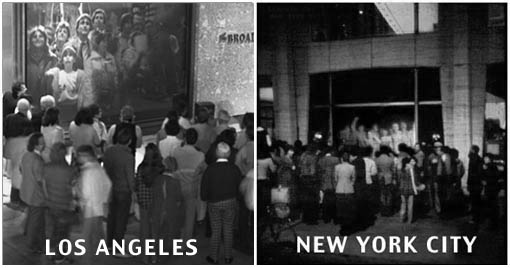
\includegraphics{figures/hole_in_space.jpg}
	\caption{Photos of the Hole in Space exhibit sites in Los Angeles and New York City.}
	\label{fig:hole-in-space}
\end{marginfigure}

\begin{marginfigure}
	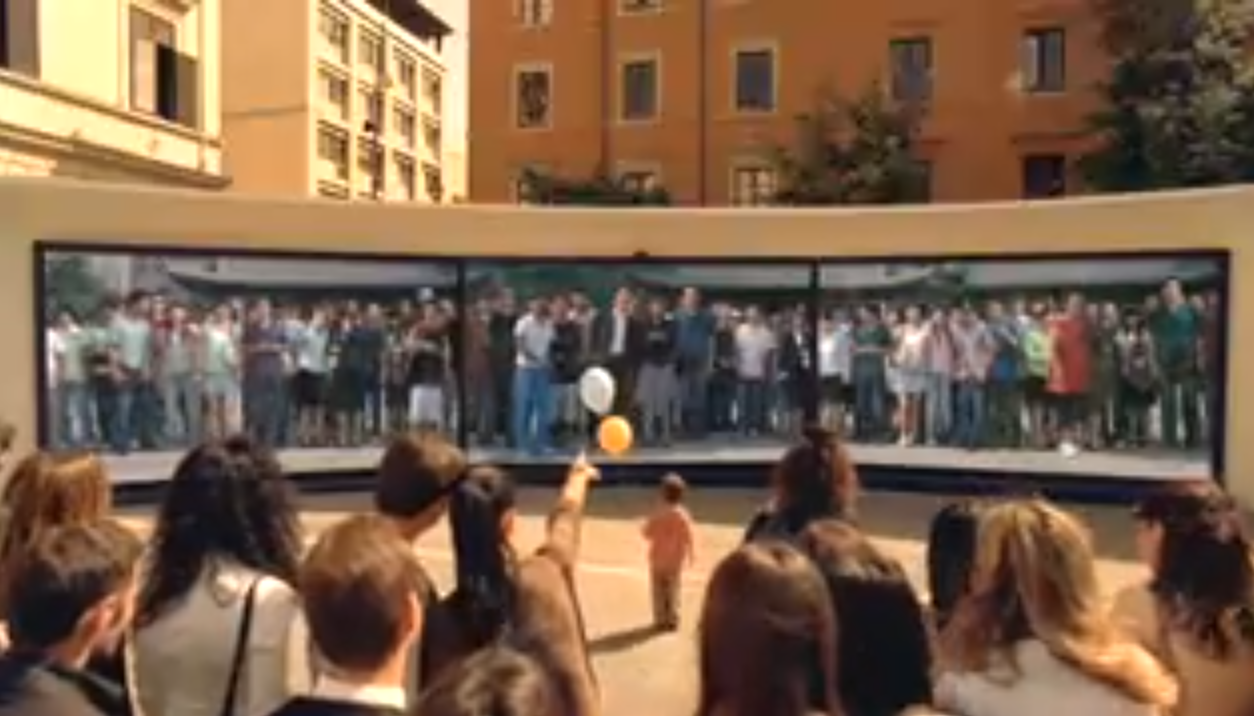
\includegraphics{figures/cisco-telepresence.png}
	\caption{Still from a Cisco Telepresence advertisement, centered on connecting an Italian piazza with a Chinese square with a seamless window.}
	\label{fig:cisco-telepresence}
\end{marginfigure}

% Despite these challenges, there's still an undeniable magic to the pursuit of recreating face-to-face communication at a distance. This magic is most poetically captured in the famous ``Hole in Space'' \citep{HoleinSpace:1980vn} piece, visually and audibly connecting a storefront in Los Angeles and New York in a way that seemed to make distance disappear. This vision is not simply aspirational, either. Tools to communicate with physically distant people either with audio alone or with an added video connection play a role in the daily lives of millions of people. This desire to experience ``being there'' with someone else is powerful and compelling.


\begin{marginfigure}
	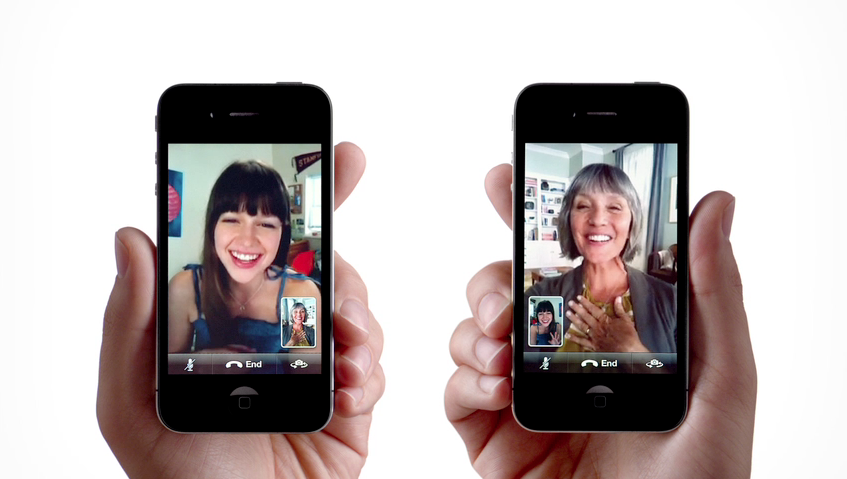
\includegraphics{figures/iphone-face-to-face.png}
	\caption{Still from an Apple advertisement demonstrating the Facetime feature to enable mobile video conferencing.}
	\label{fig:facetime}
\end{marginfigure}




\section{Complementary Communication}
This thesis addresses the design space of complementary communication systems. By this, I mean systems that aim to create a communication context shared by a group of people who are sharing some kind of experience like a presentation, performance, or discussion. Viewed this way, complementary communication systems are as old as whispering to someone sitting next to you or passing notes to a classmate. The addition of powerful personal communication technology to our everyday interactions have increased the opportunities we have to create complementary communication contexts as well as radically increased the reach a complementary communication system might have. In this context, how should we think about these sorts of systems? What goals should we have for them? In what contexts do they make sense? In particular, how should we think about the relationship between a complementary communication system in a face to face context? Is complementing a face to face interaction the same as complementing a mediated interaction?


In their famous paper, \citet{Hollan:1992tz} introduce the ``beyond being there'' approach. They argue that seeking to recreate the experience of ``being there'' was in a way an abdication of our responsibility as designers that left an important design space un-explored. In particular, they urge us to think less about ways to minimize the experience of mediation in communication, but to look instead for ways that mediation can add value to interactions. To take this perspective seriously, we need to shift away from a view of face-to-face interaction as being always better than interactions mediated by technology and instead think critically about potential limitations and challenges with face-to-face interaction and potential benefits that mediation can offer. 

\begin{marginfigure}
	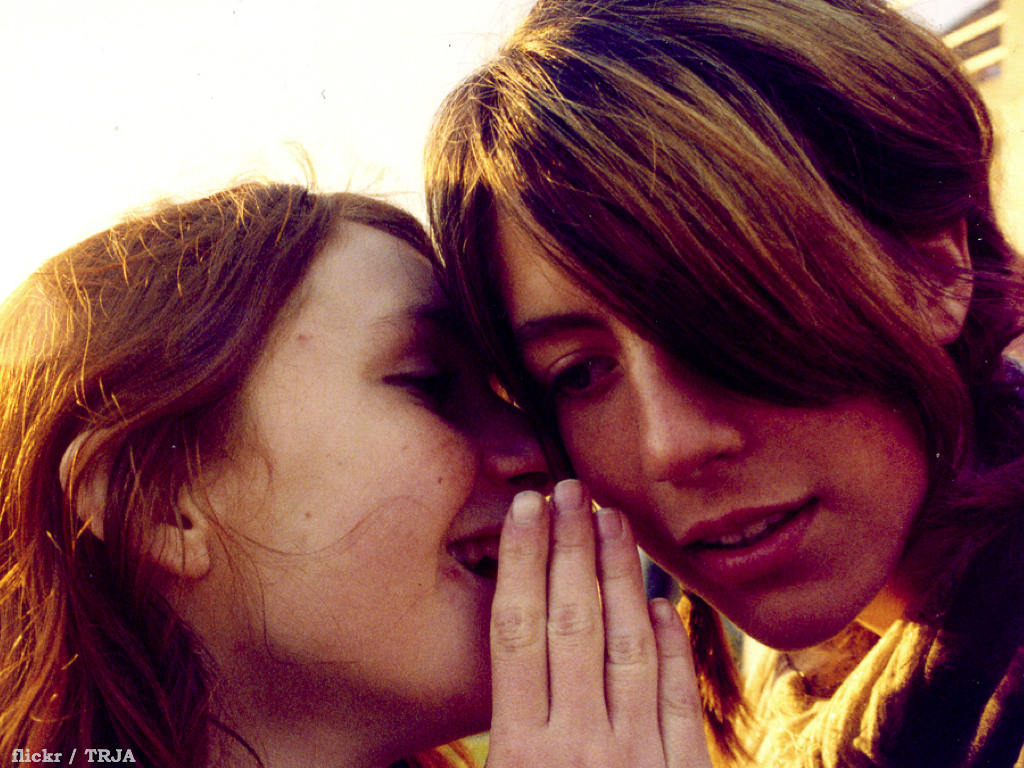
\includegraphics{figures/whisper.png}
	\caption{The original complementary communication experience.}
	\label{fig:whisper}
\end{marginfigure}


Although Hollan and Stornetta focus on creating mediated experiences that rival or surpass face-to-face experiences, in my work I show that we don't have to choose one approach or the other. If we accept the argument that being face to face is not \emph{a priori} the best experience, the strategy I employ is to add complementary communication platforms that can be used simultaneously with face-to-face communication or mediated platforms that mimic face to face interaction.


\begin{marginfigure}
	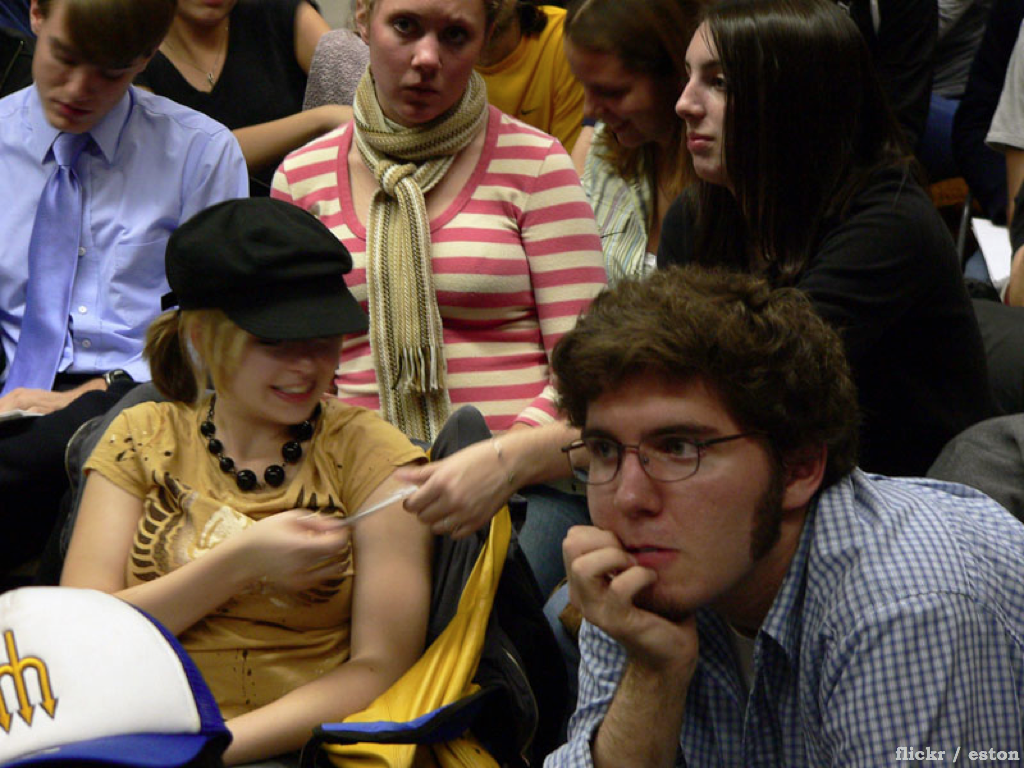
\includegraphics{figures/note-passing.png}
	\caption{The first complementary communication technology.}
	\label{fig:notes}
\end{marginfigure}


This easy equivalence between face-to-face communication and mediated imitations may seem unlikely; why should we accept that systems used in coordination with audio or video conferencing would be similar to those used to coordinate face-to-face? I will argue that a system that can effectively complement face-to-face interaction when its users could simply set it aside and rely on the (presumed superior) affordances of unfettered verbal communication likely has something to tell us about both design and face-to-face interaction more generally. If these systems can provide value in face-to-face contexts, I will show that they also provide value (perhaps even more value) when used to complement systems that seek to create experiences \emph{like} being face-to-face. Furthermore, true ``distributed'' situations are becoming less common. Heterogenous configurations where some people are co-located and others are remote and possibly alone are becoming more common. In these contexts, a system that doesn't operate effectively between co-located users is unlikely to be broadly useful, and would suffer from the disenfranchising effects we see for people who ``dial in'' to a local meeting. Thinking broadly about systems that complement both face-to-face and audio/video sharing will more efficiently lead us to systems effective in both contexts than treating them as separate cases.

\begin{marginfigure}
	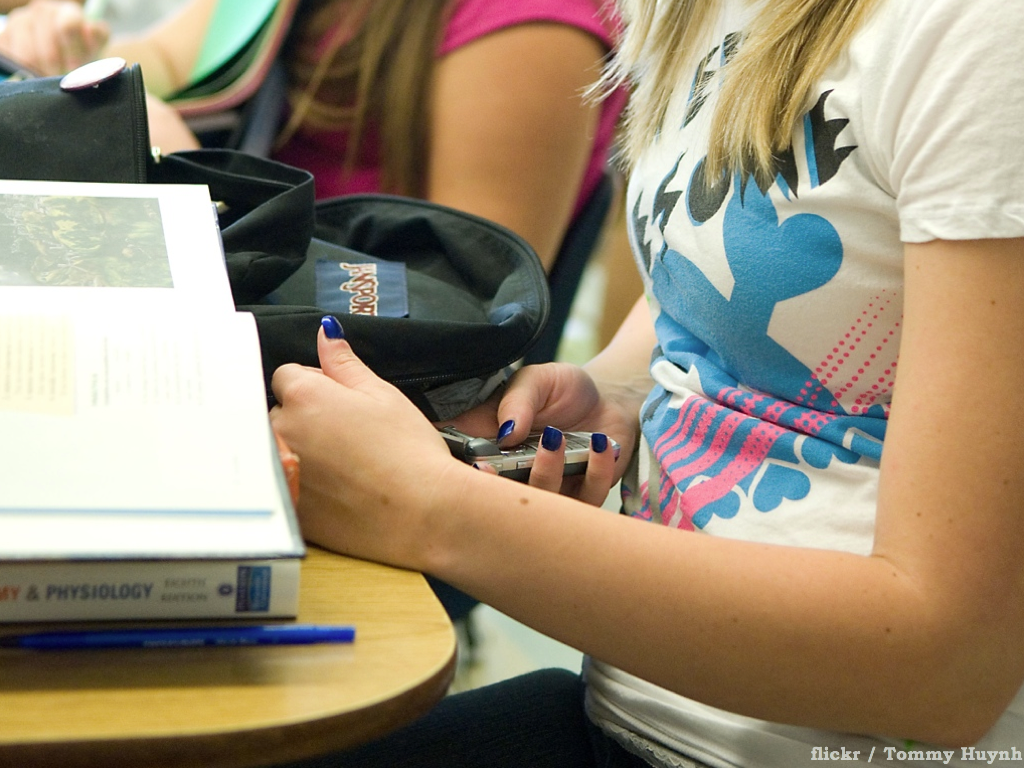
\includegraphics{figures/texting.png}
	\caption{Person to person text messaging extends the reach of something like note passing to include anyone with a phone. Phones also support multi-party conversations, increasing the size of the audience for complementary communication systems.}
	\label{fig:texting}
\end{marginfigure}




% think about listifying this section

% Many of these challenges are common sense, even if they are frequently forgotten when people argue for recreating face-to-face experiences. Face-to-face communication requires relatively explicit turn-taking; multiple speakers in a group make them all largely unintelligible. In mediated environments like chat, simultaneous conversation threads can easily co-exist for long periods of time. There are major identity implications to face-to-face communication. It is difficult to conduct any face-to-face communication without revealing significant information about your identity. In mediated contexts, there are techniques ranging from anonymity to pseudonymity to limit identity disclosing information. Participation in non-mediated interactions is ephemeral, while mediated interaction can easily be archived and represented either in context or after the fact. Participation in face-to-face situations can be limited by confidence, but mediated participation tends to be more disinhibited. \citep{Siegel:1986ve}

% is this a second order effect?
% For a variety of reasons, the power dynamics in social situations are more easily subverted in mediated environments. 

This dissertation is organized around a series of ``primary'' contexts for which I design a particular complementary communication system that enhances the overall experience. Metrics and evaluation strategies vary for each of these pieces, but each project shares a deep interest in trying to fill in the gaps of the ``primary'' interaction space by using the particular strengths of some additional mediated communication system. The goal of these interventions is to create environments where people have ways to express themselves non-verbally in addition to whatever existing communication channels exist, often audio, sometimes visual. By adding mediated communication channels to other existing channels, we can focus each channel on its primary affordances and let it do what it does best while letting the complementary communication channels fill in the gaps.


\section{From Channel To Stage}

Platforms for discussion and commenting that are outside official discourse channels have widely been referred to as ``backchannels.''  Backchannels, traditionally defined, create a space where audience members to some ``front channel'' can share information with each other, typically about the content of the front channel. \sidenote{This is in contrast with the traditional technical use of ``backchannel'', which refers to the verbal and non-verbal cues that non-speaker give a speaker during a conversation. In this usage, backchannel was a type of communication, not an actual dedicated distinct channel the way it is in this context.} This metaphor is an apt description of much of the prior work in this space, like \citep{Cogdill:2001fp,Yardi:2006uk,mccarthy_digital_2004,Rekimoto:1998jy}. I have found, however, that it is not as useful for understanding the systems I will present in this thesis. Instead of using channels, I will argue for ``stages,'' and instead of a front/back separation, I will shift to a main/side distinction. \sidenote{Parts of the section to follow are adapted from \citep{Harry:2012df}.}


In a traditional backchannel configuration, audience members can view the front channel and have a variety of backchannels available to them, each with different sized audiences and affordances. This is represented in Figure \ref{fig:front-back-channel}. Presenters, on the other hand, often have a very hard time staying aware of backchannel content if they are aware of it at all. This asymmetry gives the backchannel its outsider flavor and can lead to disrespectful and unproductive content \citep{boyd:Yo36SNyj}. This is widely recognized as a major problem with backchannels. In this way, the front/back distinction is an accurate description of existing systems, but not a situation I seek to recreate. \sidenote{Of course, there may be contexts where the front/back distinction is valuable. But since that is the predominant structure for existing tools, there are many more options for supporting that approach so I don't give it much attention in this thesis.} Mitigating this sense of separation is a major design goal in my work.





% In this configuration, the front/back channel distinction is a useful one because in a very practical sense the backchannel is usually somewhat covert or hidden and participants in the backchannel rarely have the ability or opportunity to communicate on the front channel. \sidenote{This paragraph and the rest of this section are largely from \citep{Harry:2012df}.} 

% I wonder if it's worth putting some examples here? I thiiink we can get away without, but might help ground people's thinking.

% Although this front/back channel metaphor works in situations where audience members have no access to the front channel, it is less effective in situations where the backchannel is intended to influence the front channel. 

% As will be discussed in the related work, much recent work is focused on bridging these front and back spaces and I argue through the work presented in this thesis that a new metaphor is useful for understanding how these parallel communication spaces can be configured.

To enable this shift, we need to re-imagine the nature of social interaction in these sorts of spaces. A channel metaphor implies a clear split between those empowered to broadcast, and an audience who receives that broadcast. It also has implications for how attention is managed; channels imply a model of binary attention. To find an alternative, I turn to \citet{goffman_presentation_1959} for his description of \emph{stages} to illuminate this new sort of situation. He uses the example of a waiter behaving politely with a problematic customer and then walking into the kitchen and complaining to the cook about the customer's difficult behavior. Each interaction is performative and represents the waiters' competence at performing his role appropriately for different audiences in a different setting. In the waiter example, these audiences are disjointed, and the door into the kitchen represents a gateway between the ``front'' performance space with customers and the ``back'' performance space among restaurant staff. The notion of stages shifts our attention from spaces where a small number of people can broadcast information to many recipients (like a lecture hall or conference) and instead focuses on negotiated sites of performance like the restaurant dining room and kitchen, where people can perform different aspects of their identity for different audiences. This intermediate state is shown in Figure \ref{fig:front-back-stage}. In this model, the back stage still lacks accessibility for much of the audience, and is not easily perceived by performers on the front stage.

\begin{marginfigure}
	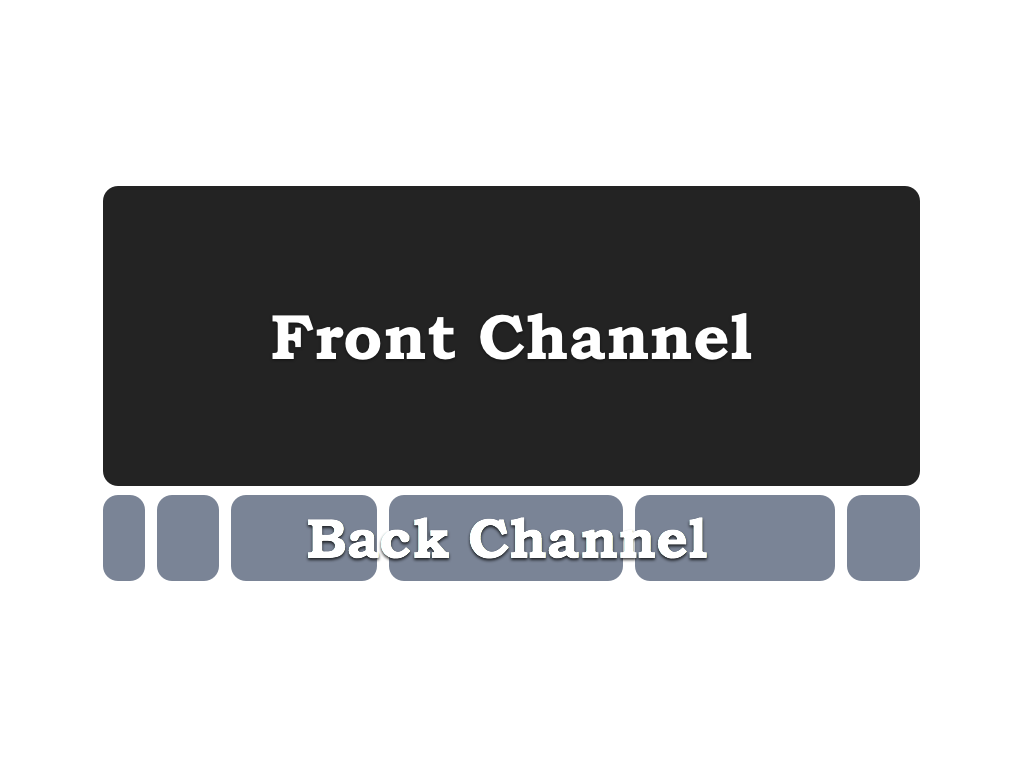
\includegraphics{figures/front-back-channel.png}
	\caption{The conceptual model inherent in a front/back channel configuration.}
	\label{fig:front-back-channel}
\end{marginfigure}

\begin{marginfigure}
	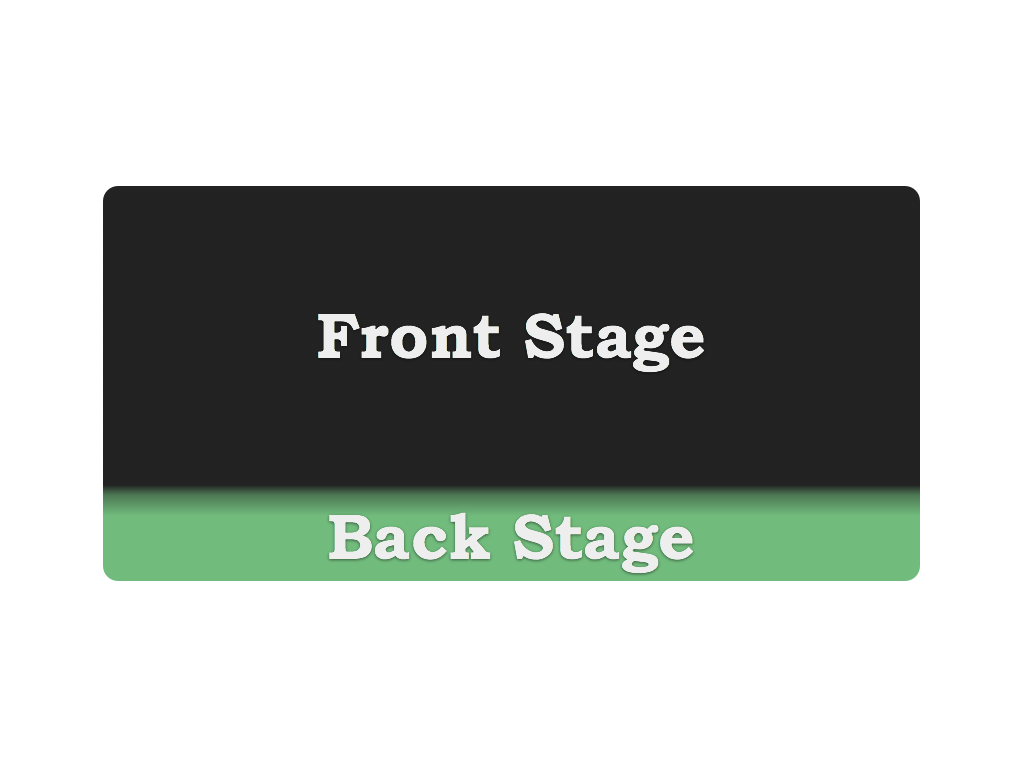
\includegraphics{figures/front-stage-back-stage.png}
	\caption{The transition from channels to stages; brings the audience closer to the performer and increases the visibility of the back stage.}
	\label{fig:front-back-stage}
\end{marginfigure}

This notion of stages is a useful metaphor to replace channels. Unlike channels, where audiences are basically invisible to the performer, stages bring the audience and performer together and create a context in which they are mutually aware of each other. Stages also shift from the notion of a small group of broadcasters and a large group of receivers, to a context where there is the potential for different performers at different moments. The notion of stages also more actively recognizes the way that audiences to a performance are themselves constantly performing in small ways, while a channel metaphor limits the audience to simply receiving a broadcast. This comprises both small performances and the potential for substantial performances. In a large lecture hall, the nature of the individual performance is not that precise. If there is an open laptop policy, audience members might be checking their email or engaging in an official backchannel.  They are able to, as Goffman says, ``get away with going away," because the act of \emph{going away} is an expected part of the front stage performance. But a shift from channels to stages is important in recognizing that even as audience members, looking at a laptop screen instead of the teacher is a sort of small performance. Furthermore, a student may raise their hand and ask a question of the teacher, thus assuming a larger role in the main stage. 

\begin{marginfigure}
	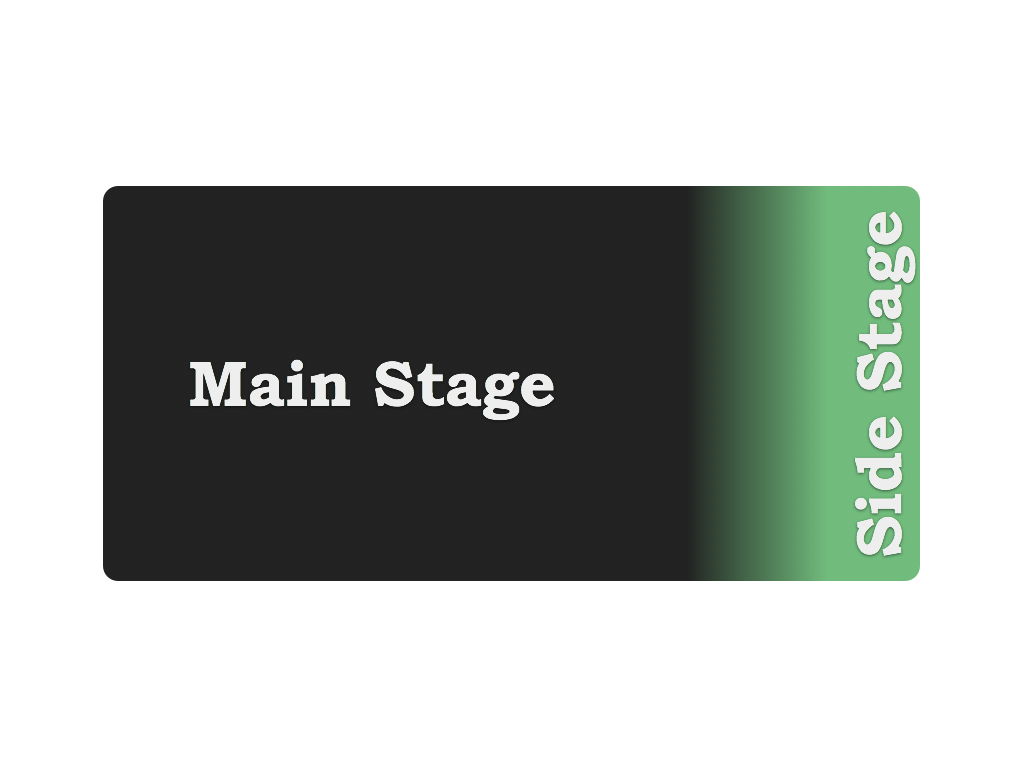
\includegraphics{figures/main-side-final.png}
	\caption{The final conceptual model that I argue for. Main and side stage are well blended and can influence each other. Main stage and side stage share an audience.}
	\label{fig:main-side-stage}
\end{marginfigure}


Although Goffman's description of appropriate performances for a specific audience is valuable, we want to avoid that front-back distinction enacted in the restaurant. Instead of having separate audiences, we want to create a space where, although the modes of performance are different, the performances are available to everyone. While in a channel metaphor, audiences are split between multiple back channels which are largely unavailable to someone performing on the front channel, stages create the opportunity for situations where the audiences for each stage can be shared. This unified audience helps us move away from the front/back distinction to a main/side distinction. In this model, performances on the main or side stage both share one large audience. By unifying the audiences, we can help avoid the problem with backchannels where they tend to assume a covert character. If side stage participation is accessible to everyone, it changes the character of the communication. Side stage performances lose some of their covert nature because they can be seen by a larger audience that includes main stage performers. Simultaneously, main stage performers can be made actively aware of side stage performances in a way that is inclusive, to help them better react to their now more present audience.

To reiterate, this change in metaphor has two components: a shift from channels to stages, and a shift from front/back to main/side. This is an aspirational shift; most of the design work in this space to date has represented the backchannel approach. But if these systems are to be an effective addition to face-to-face-type experiences, I will show how adopting this new metaphor can create effective communication experiences that encompass multiple simultaneous opportunities for engagement that create an effective, unified experience. This final configuration is shown in Figure \ref{fig:main-side-stage}. 

% Each is a performance, but the backstage is presumably more authentic. So unlike the concept of channels, which are composed of discreet information streams, stages are negotiated sites of performance around a singular situation.

% Instead of the metaphor of channel, he would refer to these alternate communication streams as stages.  When one moves from formal interactions to less formal interactions, one moves from front to back stage. When on the front stage, performance is prescribed and specific roles can be rigid.  And when on the back stage, one is more free to authentically represent themselves and their thoughts about the front stage.  He uses the example of a waiter behaving one way with a customer and then walking into the kitchen and telling the cook about the customer's difficult behavior.  Each is a performance, but the backstage is presumably more authentic. So unlike the concept of channels, which are composed of discreet information streams, stages are negotiated sites of performance around a singular situation. 






% This shift from 
% 
% 
%  But in a seminar environment, attentiveness and participation are more scrutinized because of the size and nature of the group. This suggests that integrating new communication technology into groups of smaller size might be more challenging because \emph{going away} is more difficult to politely incorporate into the front stage performance.  
% 
% 
% Communication systems used in a context where they are not the primary communication channel have historically been referred to as ``backchannel'' communication systems. Chat-oriented systems were the most popular, and have been deployed in a variety of contexts, though research has often focused on  conferences \citep{mccarthy_digital_2004, Rekimoto:1998jy} and classrooms \citep{Cogdill:2001fp,Yardi:2006uk} as fertile spaces for these sorts of interventions. More recently, tools like \emph{Twitter} have been described as a ``backchannel'' for live events. In some cases, a live-updating feed of recent tweets containing certain event-specific keywords have been projected in the space.
% 
% Although my work seems at first glance to fall into this same category of backchannel designs, I argue that a shift in the categories we use to think about these systems is important for building effective spaces. 
% 
% 
% 
% 
% In the literature about mediated communication systems used in a context where they are not the primary channel

 % Need to introduce stages as a concept here! Do the whole backchannel -> side stage transition argument here? It has to happen somewhere and it has to happen EARLY. It doesn't happen anywhere in background yet. 


\section{Design Spaces, Themes, and Theory}

One of the challenges of building technical systems as research is understanding the scope of conclusions. If you took a particular design element into a different system, would it operate in the same way? What are the relationships between the sorts of people using the system and the socio-technical structures that emerged? These are difficult questions to answer within the scope of a single project. The researcher may have solid intuition, but the tendency of the researcher is probably to see overly-general results more often than overly-specific results. One of the ways I address this is by describing a series of projects in this design space and examining design elements and themes in a variety of contexts.

This would be less effective as an approach if each of the design spaces was quite similar. The contexts I am designing for can be organized around a series of major differentiating axes:

\begin{description}
\item[Main Stage]{The medium for the main stage, e.g. the site of the primary shared experience of the audience.}
\item[Shared Display]{The presence or absence of a shared display.}
\item[Side Stage Attention]{The frequency of audience attention on the side stage. This is quite qualitative and varies across users, but each system embeds contains certain assumptions about the relative importance of the side stage to the main stage.}
\item[Audience Size]{The target audience size for the system.}
\end{description}

Table \ref{tab:project-axes} lists the research contexts covered in this dissertation, and describes each project's location on the major context axes. The variety across these axes helps show the breadth and scope of my work. 
\begin{table*}[tb]
	% \centering

\begin{tabular}{r|llll}
& Main Stage & Shared Display & Side Stage Attention & Audience Size \\
\hline
\textbf{backchan.nl} & face-to-face & yes & infrequent & 20-500 \\
Information Spaces & virtual world & yes & infrequent & 10-20 \\
ROAR & broadcast video & no & frequent & > 1,000 \\
\textbf{Tin Can} & face-to-face & no & occasional & 10-20 \\
\end{tabular}
\label{tab:project-axes}
\caption[][15pt]{Comparing the projects covered in this dissertation on the major axes that distinguish them. Projects in bold are major projects discussed in the most depth. Small project variants (e.g. backchan.nl for remote Q\&A, Tin Can Meetings, etc.) are not included.}
\end{table*}

% could I identify a set of common design elements that can be traced across all projects?
% voting
% chat
% shared display?

Although each project operates in a different context, there are a number of research themes that each project addresses. Although these themes were not identified at the start of this research stream, they nonetheless are present in all my work to various degrees. It can be challenging to identify the broader impact of design-based research (a topic I will address in more depth in the next chapter), but it is through looking at these themes in different contexts that I hope to contribute to broader discussions. These are themes that are relevant particularly to designing complementary interfaces like those in my own work, but also to many kinds of collaborative, synchronous systems, even those which aren't trying to create complementary experiences.

\begin{description}
	\item[Grounding]{My work uses shared displays in a variety of different capacities. I contend that these kinds of public displays can play a powerful role in helping to ground, in the \citet{Clark:1989uc} sense, a conversation. In particular, shared displays can provide ways to non-verbally acknowledge discourse presentations. By their very shared nature, the contents of shared displays might accelerate the creation of common ground. The different ways that these shared displays operate in my work helps provide insight into both particular design techniques to support grounding as well as the broader discussion around how common ground operates in mediated communication contexts.}
	\item[Non-verbal actions]{As a result of the drive to create a sense of ``being there'', mediated interaction systems failed to consider the ways that we communicate non-verbally, assuming that higher fidelity video and audio would be sufficient to capture that communication. I contend that our non-verbal actions in the physical world are a critical component of body language, and when creating mediated channels we should strive to create new vocabularies of action that enable people to communicate non-verbally. In much the same way that in a shared physical space we can observe people interact with objects around us, so too should people's actions in mediated systems be visible and part of supporting a sense of presence and awareness. How these action vocabularies are constructed and communicated to people is critical to the success of these sorts of systems.}
	\item[Attention]{Creating new opportunities for simultaneous commentary and communication about some shared experiences creates situations where people have to make choices about which if the stages to attend to and which stage to use for their performances. From a design perspective, there are a number of important attention related decisions to make: How is our attention made visible to others, and how does it affect their impressions of us? How do we design displays for occasional attention of users who are shifting their attention between different stages? Understanding how people think about and enact attention in situations with multiple available communication channels is critical to designing appropriate options and understanding the practices that evolve around them.}
\end{description}

This work contributes on two levels. First, by creating and deploying interfaces with particular properties, I provide concrete guidance and insight about particular specific design strategies and interfaces. This is valuable for designers and researchers thinking about how they design this variety of communication systems. I also contribute to the broader discourse about the three research themes laid out above. In each case there are both broader theoretical contributions to be made as well as specific findings that contribute to scholarly discussions about these issues.

\section{Thesis Organization}

This thesis starts with a broad background discussion about some of the methodological assumptions implicit in doing design work as research, a tour through some of the high level related work that all of my work relies on, and a more in-depth treatment of the major research themes I introduced here.

Based on this background, I will then discuss four major project areas in each of the following four chapters: Virtual Worlds (which contains two specific sub-projects for meetings and presentations in virtual worlds), \emph{backchan.nl} (a tool for managing audience feedback during live events), \emph{Tin Can} (a tablet-based platform for enhancing small group discussions), and \emph{ROAR} (a platform for very large scale audience interaction during live events). Through each of these chapters I will relate my findings back to the research themes that are laid out in Chapter \ref{ch:background}. 
\chapter{Background}
\label{ch:background}
%intro to the background section here

Although this dissertation discusses a wide variety of work, it all draws on a common foundation. This chapter will lay out that foundation before moving on to discuss specific projects. There are four components to this foundation: design as a research practice, methodology, related work, and major research themes. I will cover these in order.




% : virtual worlds, face-to-face panel discussions, small group seminar discussions, business meetings, remote information sessions, and live-event spectating

% Part of what's attractive about mediated communication systems is that there is a tremendous variety of ways to design and use them once we set aside a desire to recreate face-to-face interaction. Although in this section I've contrasted mediated communication with face-to-face communication in a way that might imply that mediated communication systems are somehow monolithic and self-similar, the survey of related systems in the section to follow will illustrate the tremendous range of potential systems in this space and demonstrate how thoughtful designs can have widely varying impacts on the experience of communication or collaboration. 

% My work takes this general design strategy of adding new communication channels in a few different directions. In this proposal, I will describe my past work looking at meetings in virtual worlds, audience-speaker interaction in presentations, and classroom discussions. I will also lay out my design for a system to support face-to-face meetings with remote participants. These research contexts vary both in the numbers of simultaneous participants, as well as their geographic configuration. Over the course of my work, I have shifted my attention from configurations where all users are remote (\emph{Information Spaces}) to heterogeneous situations where some or all of the participants are co-located (\emph{backchan.nl}, \emph{Tin Can Classroom}, \emph{Tin Can Conference}). 

% TODO Add a paragraph here that preludes some of the design as research ideas (which will be covered in more depth in their own section) as a way of saying that having these themes is part of what makes this research-worthy. 

\section{Design as Research}

Proposing a design space and arguing for its value as an approach to common problems is not, traditionally, the realm of academic research. It is a frequently taken-for-granted assumption at the Media Lab that designing novel technical systems is a natural and defensible way to do research, but outside of that context this approach is rarely accepted without argument. Given that this assumption is fundamental to my work, it seems useful to address this epistemological question from the start.

Design as research is clearly being conducted in a variety of contexts using a variety of methods, yet there is very little discussion or agreement about the fundamental aspects of how that work is conducted and what we can learn from it. Traditionally it is tolerated, provided that the primary argument for its contribution to the wider discourse is based on a justification from another research field. In computer science related fields, efficiency and technical complexity are reliable ways to argue for the quality of work, even work like mine where novel systems and interactions are described. This has a warping effect on the sorts of systems that are built and studied because there needs to either be a technical challenge in the solution or a way to easily judge the efficiency of the solution relative to existing methods.

Although there are ways to frame my work in those terms, I do not view those as particularly effective ways to judge my work. Instead, in this section I would like to make a positive argument for why building and testing systems may be the \emph{best} approach for certain kinds of research questions. I will describe the sorts of contributions one can make working this way and contrast this approach with other approaches dominant in the fields of human computer interaction, computer mediated communication, and computer supported cooperative work.

% TODO This is a stupid title, especially relative to the section title. FIX IT.
\subsection{Engineering as Research}

% can I get away with these claims? if I wanted to be serious about it I would do a some lit review statistics. but I don't really want to get bogged down in that. Lets see if I can get away without it.
It is a gross simplification, but let us separate work in the field of human computer interaction or computer supported cooperative work into three general categories: technology-enabled sociology and psychology, studies of systems in-the-wild, and design of new systems. In the first category, researchers seek to answer the kinds of questions typically of interest to sociologists and psychologists, but deploy technology to allow them to answer questions they have not been able to answer in sufficient detail in the past. This work focuses primarily (but not exclusively) on drawing conclusions about the behavior and experiences of either individuals or collections of people. Studies of systems in-the-wild are, in contrast, more focused on understanding the relationship between the technology and its use, often described as socio-technical systems. Finally, there are researchers who design and build novel systems and then study them. I describe this final category of researchers (of which I consider myself a member) researchers-as-designers. 

These last two categories are deceptively similar. After building a novel system, does one simply run a study on that system like a researcher who didn't build the system themselves? This suggests a critical thought experiment: if the researcher-as-designer could simply imagine a system into existence that looked exactly like the system they wished to study, would that compromise the research in any fundamental way? Put another way, does the actual design and implementation process actually add value to the research or is it just an overhead?

Although provocative, the thought experiment is subtly mis-framed. Technical artifacts can never really be imagined into existence because their creation is a constant negotiation between the properties of the tools used to create it, the environment in which the design happens, and the reactions the designer has to their own work. In practice, the artifact that comes out of a design process is the result of a lengthy iterative process, even in design processes conceived as iterative. Simply creating part of an artifact and integrating into another part causes a re-evaluation of those parts in a way that causes designs to drift from their original models. The time spent in the design and implementation processes can be seen as critical for producing a viable design. If we desire to study systems that don't already exist, there is simply no way around spending time on the design itself because our ideas about what the design could or should be before entering those process cannot become real without any intermediate steps, and if they could they would be unlikely to meet any of the original design goals. From this perspective, we view the development process as a fundamentally necessary cost of creating any novel system. 

% took this from some older writing I did - don't need to dig into that particular account because readers other than Wanda won't be familiar with it.
% The second approach is to turn to Schutlze's confessional account of her dissertation field work in which she struggled with the practical realities of trying to be a participant in the work lives of her informants without injecting her own in-progress conceptualizations of their work experience and without her researcher identity becoming compromised by her affiliation with a specific work group in the organization. Yet, we (I think rightly) value her attempts to not simply sit outside the process she's studying, but to take part in it. This is fundamental to participant-observation as a methodology. 

An alternative approach is to consider the distinctive values of the design process as a research process. In some fields, we expect that the researcher will become deeply embedded in the process on which their work focuses. In these fields, putting yourself at a distance and insisting that you can simply observe without being part of that process is often viewed as naive. Yet when we shift our focus to creating novel technical artifacts, we prefer to isolate either the users (as in lab studies) or the treat the artifact itself as stable (as in studies of the use of existing artifacts \emph{in situ}). It seems only natural to say that claims about the design of socio-technical systems can be easily augmented by a long-term, rich participation in that exact process. Playing the role of the active participant in the process grants us credibility and real analytical leverage. I don't mean to say that one can't make arguments about design choices made in a design process without being a participant in it--you certainly can--but being a participant in that process provides important insights that we are unlikely to find if we treat the technology as the black box output of an historical design process conducted by others. 


% this paragraph needs to be about WHAT ARE THE INSIGHTS FROM THE DESIGN PROCESS?

It is difficult to precisely identify the sorts of contributions that would not be possible without engaging in the design process because there are few examples of a team doing novel design work and handing off the result to a separate researcher and comparing their results. We do have a large body of research on systems conducted by non-designer researchers, but there's nothing to systematically compare it to. I hope instead that my work highlights how the researcher-as-designer can operate effectively in both roles and serve as a starting point for a broader discussion about why designing and studying systems is as valuable a research strategy as studying existing systems. \sidenote{Designing and building systems can take a substantial amount of time, especially if you hope to deploy those systems \emph{in situ} instead of in lab contexts. If papers are the main output metric for a researcher, this approach is not necessarily an efficient way to generate papers, since few conferences will accept papers on the design or development of a novel system without an attached `study'. This might help explain the waning popularity of this sort of research.}

If we accept that conducting design and development are valuable research processes, we must consider the challenges to this kind of work. If we hope to avoid the limits of studying design work in decontextualized lab situations, then we need to find situations were our system might credibly be used ``for real.'' The best situations are ones in which people interacting with and through the system can do so in the normal contexts in which they might interact with such a system: using their own devices, in places that are familiar to them, and with people who they might normally use such a system with. These contexts can be quite difficult to secure. Some systems require a certain scale to reveal meaningful results; had a researcher designed \emph{Twitter}, they would have been very hard-pressed to find a context in which they could study it in a legitimate way. These constraints are also acute when designing for business contexts. Deploying research software in business contexts poses risks for the business in terms of data security as well as ethical concerns about businesses compelling their employees to use the system. Although this limits the kind of design work the researcher-as-designer might credibly study, these constraints are notably different than the constraints on researchers who study existing in-the-wild systems. In many ways, these biases are nicely complementary:

\begin{table}[tb]
\begin{tabular}{r|l}
\textbf{Researcher-as-Designer} & \textbf{Researcher} \\
using novel technology & using existing technology \\
not widely deployed or available & popular/widely used \\
smaller, bounded user groups & larger, fluid user groups \\
extrinsically motivated users & intrinsically motivated users\\
rougher edges & well polished\\
consumer-oriented & consumer or professional\\
bounded use durations & potentially unbounded use durations\\
internal process traces & publicly observable process traces\\
\end{tabular}
\label{table:research-focus-comparison}
\caption{Comparison between the kinds of technical contexts that the researcher-as-designer typically studies compared to the researcher.}
\end{table}

On most of these axes, it is not that researchers are incapable or uninterested in studying the kinds of systems that the researcher-as-designer studies, but that (for a variety of systemic and historical reasons) they have gravitated towards these particular themes. Whatever the reason, these differences add to the value of the researcher-as-designer approach. Even if taking the role of researcher-as-designer takes a substantial time investment to create the systems being studied, if it reveals insights about new kinds of systems that traditional researchers might not pay attention to then it can be a valuable approach. This is most true with respect to the properties of the technology in the system. The researcher-as-designer can also be conceived of as mapping terrain that the designer-as-professional and other researchers will later cover when the technology becomes more widely accessible or viable. Furthermore, the kinds of deep data collection possible with custom-engineered systems open up a variety of analytical options that are often not possible when trying to collect data from publicly available and usually corporate-controlled contexts like \emph{Facebook} or \emph{Twitter}. Unlike data collected by corporate actors, these data collection processes are subject to institutional review and access to the data is not contingent on the arguments being made with the data being acceptable to corporate actors. This is a further reason why the researcher-as-designer can find insights that might not be accessible in systems designed by others.

This is not an argument for one approach to replace another; both approaches can easily co-exist. However, because I rely so heavily on this approach in my work, I want to present the reasons why working in this particular way is a valuable complement to dominant research strategies. This is particularly relevant in a Media Lab context where building systems is a taken-for-granted component of our work, but we rarely seek to justify it on its own terms to other researchers. Hopefully this section can serve as a start to a broader conversation about whether and how this research strategy can make contributions that are respected and valued outside our own Lab.

\section{Methodological Approach}
% ??? Could talk about studies in authentic contexts and do the whole critique of lab-based studies here. Probably not super relevant, and a bit risky since a lot of the stuff I'll end up talking about doesn't have particular studies attached to it. 

% other potential topic: broad ideas about how people and technology interact and what the focus of study is?

% there's a risk here at being all about what it's not versus what it is.
% I don't want to get too deep into just griping about the challenges of
% in situ work. however, it's worth making the critique of other approaches. 

This work is not a single monolithic study and so it does not share a single methodology across all its components. Still, there are some common methodological approaches that I would like to highlight. In particular, I would like to draw attention to the differences between the sorts of design research that I aspire to conduct, and describe how this approach contrasts with more traditional approaches. 

Perhaps the best way to contrast my approach to the approach of much of the systems research literature is to describe my approach as \emph{in situ} to contrast it with what I would characterize as a traditional \emph{ex situ} approach. Because of its roots in experimental psychology, studies in the HCI and CSCW fields are typically designed around normalizing as many as possible variables to focus on particular independent variables. Studies are typically conducted with subjects recruited independently, who are given a particular scenario with defined roles and tasks to complete. There are usually rewards involved, and sometimes those rewards are tied to performance. \citet{McGrath:1984un} describes these as ``quasi-groups'' and claims that they ``are the \emph{least natural} of the set of groups discussed so far'' (emphasis original). The basic axes that McGrath uses to separate groups splits them with respect to temporal scope, activity scope, whether the group frequently handles their current task, and how the group is composed. On all of these axes groups composed for lab studies are extraordinary; they share few common features with the groups that my work actually hopes to address. As a result, conducting lab studies would provide little valuable insight into group-oriented systems.


Setting aside the properties of the group, the setting of lab studies is also quite problematic. Participants are expected to set aside their prior motivations and replace them with a desire to follow instructions and be a good participant. Studies in this space are rarely this extreme, but the Stanford Prison Experiment \citep{Haney:1973wf} and Milgram's work on authority \citep{Milgram:1983vh} show how powerful this effect can be. Even when the researcher isn't trying to push subjects, there is nonetheless a passive and subtle pressure to respect the researcher's work and help them generate positive results. This is exacerbated when there is a prior relationship between the study subjects and the researcher, which is all too common. 

Studies conducted in an \emph{ex situ} lab situation also tend to extract individuals from their existing socio-technical infrastructures. Few systems are used in a vacuum. Even a system as simple as a traditional website can be viewed in quite different contexts: phones, tablets, and computers all have quite different interaction properties, and are often configured in distinctly individual ways. Yet in lab studies we tend to insist on participants using a specific configuration that is likely to be foreign to their own experience outside the lab. We also force a certain level of focus on study participants. Although it is common to frequently switch between applications and interaction contexts, researcher expectations in a lab context will significantly discourage this sort of behavior, even though it is natural and common \emph{in situ}. 

Lab studies also tend to limit the sorts of systems that can be fruitfully studied in terms of frequency and duration of use. We expect participants to use an interface intensely for a short period of time measured in minutes. Interfaces that are intended to be used occasionally over longer periods of time are not easily evaluated in lab studies and so an over-reliance on lab studies will tend to exclude those classes of systems. This is an example of the most insidious sort of influence that the pressure to conduct \emph{ex situ} experiments has on research: systems that are hard to study in terms the research community will accept will simply be built less frequently. Researchers must constantly make strategic judgements about what sorts of work they do and whether it will be be viewed as a valuable research contribution. 

In my work, I try to balance the focus of \emph{ex situ} studies in recent literature with a strong push to create systems that can credibly be studied \emph{in situ}. Mirroring my earlier argument for the researcher-as-designer to complement the researcher, \emph{in situ} research can more effectively address different sorts of research questions at a different scale than \emph{ex situ} research.

% short focused used -> long term, potentially occasional use
% fixed platform, unintegrated -> diverse platforms, integrated
% controlled variables -> uncontrolled variables
% unrelated people -> related people

% This distinction between \emph{ex situ} and \emph{in situ} research is in some ways a shift from a positivist perspective to an interpretivist perspective. A positivist focus on building predictive models is simply not a natural fit for addressing the sorts of questions.

% this will necessarily translate into an argument for interpretivism which I'm not sure I really want to get in here? In any event, this will bog me down forever so I'm going to just move on. 


In contrast, my work focuses on recruiting people who are performing an existing task (e.g. asking questions of panelists at a conference or participating in a classroom discussion) regardless of their participation in a study or not. Indeed, in the \emph{backchan.nl} case there was not a formal study at all, simply organizations that requested access to the system. Their desires and goals predated my technical interventions. The system has continued to be used by various audiences to meet an actual practical need. This demonstrates the stability of both the concept and the technology. Although we should not expect that all \emph{in situ}-style systems should continue beyond the life of the project, their viability should represent a research contribution commensurate with the challenges of building durable and complete systems that operate effectively beyond a tightly controlled \emph{ex situ} environment.


% Contexts that share these pre-existing motivations are great spaces to explore complicated context-sensitive research questions. Unlike lab studies where 
% 
% This distinction is important because our work often seeks to address questions around 




I am far from the only person conducting work in this manner. There is a long history of \emph{in situ} work. The vast majority of the work described in the \emph{Channels} section in related work is conducted this way. \emph{Thunderwire}, \emph{Cruiser}, and \emph{Portholes} are prime examples of this approach. Within a Media Lab context, it seems natural and uncontroversial to work in this fashion. But when looking at research outside the lab it can be easy to feel like this approach isn't broadly valued. A common criticism of work at the Lab is that it is all about presenting a system as ``cool'' and not about addressing any issues that research communities are interested in. Making this argument here is my way of trying to leave behind an argument that might be useful for later researchers at the lab struggling to justify their work to outside audiences that prefer empirical approaches or studies that focus on existing successful platforms.


\section{Research Themes}

The projects in this thesis are connected by a series of research themes. All of the projects speak to these themes in different ways. In this section, I will introduce these themes in more detail.

\subsection{Grounding}

Grounding was introduced as a concept by \citet{Clark:1989uc} to better understand discourse processes. Clark and Schaefer sought to model two party conversations, with a focus on how conversants construct a \emph{common ground} between them. The notion of a common ground that represents the body of understanding shared by conversants was a feature of many discussion models at the time. However, the process by which a concept moved from being understood by one participant in a conversation to both participants was unclear. Many models argued that by simply uttering a sentence, its content were immediately part of common ground. Using a corpus of real spoken conversations, Clark and Schaefer propose an alternative model where all contributions to common ground must be accepted by the other conversant before they become part of common ground. This acceptance need not be an utterance itself; an utterance that builds on a previous utterance can represent an implicit acceptance. \sidenote{Backchannels also play an important role here. Nodding or showing obvious confusion can be non-verbal, visual ways to accepting a contribution or rejecting a contribution. Taking away these backchannels can make it very difficult to judge whether common ground is being created or whether you audience is silently rejecting your attempts to add to common ground.}

In my work, the Clark and Schaefer model has a number of implications for my work. As Clark identifies in later work \citep{Brennan:1991wk}, mediated communication channels can inhibit the formation of common ground in a variety of ways. A slight addition of latency, as is common in voice or video conferencing can make turn-taking challenging which leads to longer utterances and rarer acceptance turns. Furthermore, Clark's models are primarily for two person conversations. As the number of people involved increases (as is true for all my work), the challenges become even more pronounced. Thus systems that can help provide ways to come to group understandings about goals, topics, or process can be quite powerful. 

An interest in promoting the construction of common ground is not limited to mediated technical systems. Having a well defined group process can play a major role in accelerating this process, whether it's through hand signals for signaling approval or disapproval or structures for transitioning between topics. A simple understanding like ``if I stay silent in a discussion it represents agreement; if I disagree, I must speak up'' can help alleviate some of the challenges of common ground in group work. 

A common theme both in my work and other approaches to managing the challenges of creating common ground in a group is exporting group state into the environment. Post-it notes in design processes represent a similar strategy; by moving ideas onto physical objects in the environment, we are not over-burdening the audio channel with all the content of our ideas, while also creating representations that are durable and shared. A drawing that everyone can see may mean more to its author than to everyone else, but is still more a part of common ground than only verbal contributions. My work frequently uses a similar strategy: shared displays that can be seen by all participants and whose content is generated by the group. By using a shared screen, it becomes possible for group interactions to be represented in a way that they can rapidly become part of common ground without requiring verbal utterances. In each of the projects described in this thesis, I will show how this process works (or fails to work in some cases) and argue that communication tools that create side stage spaces can help mitigate the challenges of grounding in mediated communication.


% start with an introduction to what grounding means traditionally: how we come to an understanding
% clark identifies in the later paper the different ways that technologies for mediation can impinge on the natural grounding processes


% there are limits to clark's initial analysis: how to scale to more people? 

% also are there ways that technology can support grounding? coming to a shared understanding as a group of where we are and where we're going?

% as mcclark points out, process is a part of this as well. structures that set expectations for process can have an impact

% we also see an interest in grounding in systems that seek to export discussion state into physical artifacts, like ideo's design methods or affinity diagrams


% close with a quick outline of the overall argument re grounding which is
% that having SHARED screens and additional challenges can help lubricate creating a sense that we're all on the same page

% talk about it re: voting too, in that voting creates a sense of community membership

\subsection{Non-verbal actions}

While grounding and common ground are concepts primarily focused on oral and written utterances, non-verbal actions have an important role to play in this process as well. When people lament the lack of ``body language'' in mediated communication, it is partially a complaint about the difficulties of building common ground in the absence of easy non-verbal acknowledgements of a contribution. Non-verbal actions are much broader than backchannel acceptances, though. They also include actions like nodding, looking attentive, fidgeting, taking notes, hand-raising, and so on. Although the lack of these actions in mediated environments is frustrating, we can't easily replicate them all in a mediated context. Non-verbal ways of communicating in non-mediated contexts have arisen over a long period of time, and are frequently culturally specific. Deciding which non-verbal actions to support, how to represent those actions, and understanding how these actions are understood are at the heart of this research theme.

There is an instinct in this space to simply recreate the non-verbal actions that serve us so well in un-mediated contexts. In the same way that interface designers often fall back on physical textures to evoke the properties and uses of the physical object in a digital context\sidenote{Apple is the high profile company to use this practice extensively, with their leather-textured calendar application, bookshelf background for ebooks, and brushed metal window effects. This technique is often called ``skeumorphism'' and is widely derided by user interface designers, but nevertheless is increasingly common in both desktop and mobile applications.}, designers of social systems can sometimes employ a similar strategy. This kind of social skeumorphism is quite common in the virtual world domain, and I will discuss its failings in more depth in Chapter \ref{ch:virtual}. On the web, however, such skeumorphism is harder. Although many of our non-verbal actions take their names from physical actions like ``poke'', ``raise hand'' or ``flag'', we have also seen a wide range of new kinds of actions like ``upvote'', ``like'', and ``retweet.'' These actions, like their non-mediated predecessors, have slowly evolved to carry their own novel meanings and connotations based on context.

Although non-verbal actions of this sort are prominent components of mediated social systems, they are rarely called out as an explicit research area in this way. Nevertheless, a review of the systems literature later in this chapter will reveal that much of the work in this space employs carefully chosen non-verbal actions to facilitate their design goals. By calling out this component of a thoughtful design, I hope to call attention to the important role that non-verbal actions can play. In each of the projects I discuss, I will call out the non-verbal actions that I employ and discuss their efficacy.


 % grounding is primarily about utterances both oral and written. in non-mediated communication, there is a broad vocabulary of non-verbal actions (eg nodding, attention, fidgeting, looking at watch, taking notes, hand-raising, anxiety, etc) in mediated communication, we have to make careful choices about what sorts of actions we want to create and how to represent them in a meaningful way. 

% different approaches to this problem: social skeumorphism or new actions

% non-verbal actions are not typically a research theme unto themselves; there is little work that focuses specifically on this. still, a review of the systems literature in this chapter reveals that non-verbal actions play a substantial role in the design of many systems (etc)

% ???


\subsection{Attention}

Attention, for our purposes, is best understood not as an innate characteristic of someone's behavior, but as a value-laden socially situated performative behavior. ``We are always to a certain extent in a state of distraction,'' according to sociologist Emile Durkheim. \citep{Durkheim:1974tc} Every situation is composed of stimuli that disrupts some fictional conception of undivided attention.  Likewise, every situation requires some aspect of performance, as individuals are required to communicate their attentiveness in response to specific social contexts. \sidenote{Originally from \citep{Harry:2012df}.} Although in many situations we might expect ``attention'' from our audience, what we really expect is an appropriate performance of attention that satisfies social norms. This performance is related to, but not exactly identical to what someone is focused on at specific moment. The performance of attention is a necessary indirection because we cannot ever really know for sure what someone is focusing on, so instead we rely in social situations on proxy performances.

In this thesis, I describe systems that complement another communication channel. In these contexts, I am interested in two main aspects of attention: how do people make choices about what to focus on in their environment and how do representations of attention shift in the presence of these new ways to be involved?

This research theme is partially a response to a frequent criticism of this sort of work. Won't creating new stages simply devalue attention on the main stage? Because attention is a social construct, part of the goal with each of my projects is to show how creating side stages tightly related to the main stage can make it easier to reconfigure expectations about what attention looks like. In spaces like this, focusing on a mobile device, laptop, or projected image can shift from being a display of inattention to become another way of attending to an important shared experience. This shift is important, because my work shows that many people can feel disenfranchised by main stages in different contexts and new stages with different affordances can help boost overall engagement.

This takes a shift in attitude. Instead of assuming that being in a privileged position on the main stage means you deserve the full focus and performed attention of all audience members, it is more productive to view people's focus as fluid; capable of shifting often and easily among a variety of targets on a moment-to-moment basis. A well designed side stage is one many possible targets for attention in a space, and in the best situations can contribute to the main stage making a focus on either the main or side stage a way of attending to the same underlying experience. But because attention is fundamentally performative, this change will require shifting social understandings of different ways of being part of a shared experience.

Across each of my projects in this thesis, I will try to address how attention is understood and constructed, as well as describe the processes by which people make choices about attending to either the main stage or the side stages.


% I don't really have a clue of what to do here - what am I trying to say?

% coexisting with other systems or in a face to face situation naturally means dealing with questions of attention

% pull in the content from the tin can chapter here? that's the best we've 
% really got. 

% basically I want to say:
% 1. interested primarily in arguing that attention is performative
%		this means that to some extent our notions of what attention means will shift with the context; already in some places, attending to a device is viewed not as inattention, but an alternative form of attention
% 1. in the same way that multiple spaces to perform supports people with different preferences, multiple ways to attend supports people with different preferences
% 1. 
% 1. will argue over the course of these projects that... attention shifts between, having multiple ways to engage increases attention to the primary shared experience
% 1. 

\section{Related Work}
Designing new systems for collaboration and communication, as opposed to studying existing systems, has long been a major stream of HCI and CSCW research. This section will summarize the most salient past work in this area, although little of this work is recent and responsive to the significant shifts in the way people use technology to communicate, collaborate, and play. 

For a variety of reasons, there has been somewhat of a shift in interest away from the kind of hybrid face-to-face/mediated experiences I create towards building and studying systems for asynchronous experiences between much larger numbers of people. The advent of research on mass collaboration systems like \emph{Wikipedia} (e.g. \citep{Kittur:2007up}) and ``crowd sourcing'' (e.g. \citep{Bernstein:2010wk}) is part of a larger shift away from what was once the center of gravity of systems research. This shift is a natural response to changes in both technology and the common experience of modern collaborative technology users in a web-oriented world where asynchronous interaction became the norm. But the experiences these sorts of studies focus on are predominantly single-channel and asynchronous. This is in stark contrast to my work, which is concerned with the properties of multi-channel synchronous experiences. 

In this work, I focus on interactions within groups both small and large, co-located and remote, but always co-temporal. Although interesting new sorts of work and communication structures are evolving in the asynchronous domain, we should think not just about how to marshal large numbers of people, but about how small groups of people who know each other work, recognizing that much of that work happens face-to-face or co-temporally while geographically distant. It is not effective to treat these interactions as a simple increase in tempo on asynchronous interactions. In synchronous systems, it is much more important to understand how we are perceived (and can control those perceptions) by others. In asynchronous systems, these issues are minimized; we experience others through their actions on shared objects like documents. 

% In my work, I seek to create richer representations of people and better-support person-person interaction instead of person-document-person interaction. 

My survey of related work is organized into three major design strategies: translucence and awareness, adding new communication channels, and design techniques to help people reflect on their own participation and the participation of others. These design strategies have influenced my own design process and have important findings related to my three main research themes: grounding, actions, and attention. As I discuss each design strategy, I will point out their connections to the main research themes. Table \ref{tab:related-work} summarizes the major work covered in this section, and its relationship with the three themes. After a discussion of work primarily in the systems literature, I will also cover related theoretical contributions and perspectives that influence and contextualize my work.

\begin{table*}[p]

\begin{tabular}{lrcccl}

& & \begin{sideways}Grounding\end{sideways} & \begin{sideways}Actions\end{sideways} & \begin{sideways}Attention\end{sideways} \\
\midrule


\multicolumn{2}{l}{Social Translucence} & & & & \\
\midrule

& \emph{Loops, Babble, Lecture} &$\bullet$& $\CIRCLE$ & $\cdot$ & \citep{Erickson:2000kb} \\
& \emph{Group SketchPad} &$\bullet$& $\CIRCLE$ &$\bullet$& \citep{Gutwin:2002tf} \\
& \emph{CafeCK} &$\bullet$& $\CIRCLE$ &$\bullet$& \citep{Ackerman:1995tj} \\
& Airplane Cockpits & $\CIRCLE$ & $\CIRCLE$ & $\CIRCLE$ & \citep{Hutchins:1995ud} \\
& \emph{ClearBoard} & $\CIRCLE$ &$\bullet$& $\cdot$ & \citep{Ishii:1992bq} \\
\midrule


\multicolumn{2}{l}{Channels} & & & & \\ \midrule & Class Backchannels &
$\cdot$ & $\cdot$ &$\bullet$& \citep{Yardi:2006uk} \\ & Conference
Backchannels & $\cdot$ & $\cdot$ &$\bullet$& \citep{mccarthy_digital_2004} \\
& Semi-Public Displays &$\bullet$&$\bullet$&$\bullet$& \citep{Huang:2003ef} \\
& \emph{Rendezvous} &$\bullet$&$\bullet$& $\cdot$ &
\citep{kellogg_leveraging_2006} \\ & Audio Backchannels & $\cdot$
&$\bullet$&$\bullet$& \citep{Yankelovich:2005bx} \\ & Fragmented Social Mirror
& $\CIRCLE$ & $\bullet$ & $\bullet$ & \citep{Bergstrom:wl} \\ &
\emph{VideoWindow} &$\bullet$& $\cdot$ &$\bullet$& \citep{Fish:1990fn} \\ &
\emph{Thunderwire} & $\cdot$ &$\bullet$& $\CIRCLE$ & \citep{hindus1996thunderwire} \\
& \emph{iCom} &$\bullet$&$\bullet$&$\bullet$& \citep{Agamanolis:2003wc} \\ &
\emph{Portholes} &$\bullet$& $\cdot$ &$\bullet$& \citep{Dourish:1992fu} \\ &
\emph{Cruiser} & $\cdot$ & $\CIRCLE$ &$\bullet$& \citep{Fish:1992vz} \\ & GDSS
& $\CIRCLE$ &$\bullet$& $\cdot$ & \citep{nunamaker_electronic_1991} \\ &
\emph{Cognoter} & $\CIRCLE$ & $\CIRCLE$ & $\CIRCLE$ & \citep{Tatar:1991jq} \\
\midrule \multicolumn{2}{l}{Reflection} & & & & \\ \midrule & \emph{Second
Messenger} &$\bullet$& $\cdot$ & $\cdot$ & \citep{DiMicco:2007ie} \\ &
\emph{Meeting Mediator} &$\bullet$& $\cdot$ & $\cdot$ & \citep{Kim:2008ip} \\
& \emph{Conversation Clusters} &$\bullet$& $\cdot$ &$\bullet$&
\citep{Bergstrom:2009fe} \\ & \emph{Conversation Votes}
&$\bullet$&$\bullet$&$\bullet$& \citep{Bergstrom:2009ej} \\ &
\emph{Conversation Clock} &$\bullet$& $\cdot$ &$\bullet$&
\citep{Bergstrom:2007je} \\ \bottomrule \end{tabular} \vspace{3em} \caption{A
summary of the major related work to be discussed in this section and its
relationship with the main research themes. } \label{tab:related-work}
\end{table*}

\subsection{Translucence \& Awareness}

This work owes a clear debt to the work of \citet{Erickson:2000kb} on social translucence. Their work intersects with my action and grounding themes. \emph{Social translucence} is a design strategy that aims to create ``digital systems such that people's presence and activity, made appropriately perceptible, will create accountability and more easily coordinated action''  \citep{Kellogg:2002ts}. They call their example systems designed for this purpose ``social proxies'' that use ``abstract visual representations ... to portray information, in addition to contextual information provided by the other common traces of user activity in mediated communication environments (e.g. persistent conversation).'' In each of their projects (Babble, Loops, Lecture, Auction, etc.; \citep{Erickson:2003td} is a nice overview of these projects), they seek to promote a sense of ``collective awareness'' where each person using the system has a sense of the actions of others in the system and appreciates that this awareness is mutual. 

We share an interest, in my terms, in how we can construct meaningful actions in mediated social spaces and how we can understand how public displays can help ground collaborative and discursive processes. As Erickson and Kellogg point out, this has been a topic of interest both direct and indirect for quite some time in the systems literature. Their work nicely complements work by \citet{Gutwin:2002tf}, who present a framework for thinking about the ways the workspace awareness through actions can be constructed and presented.  \citet{Ackerman:1995tj} share this interest, too, but focus on representing overall system activity as an inducement for broader participation. This is an important finding, and one I echo in my work, particularly when it comes to a public, optional system like \emph{backchan.nl}. Distributed cognition, as described by \citet{Hollan:2000ud} represents another productive way to think about these processes; by fostering a sense of mutual awareness we can support the kinds of process that \citet{Hutchins:1995ud} describes in flexible communication systems. I see my work as a continuation of these past approaches to representing activity. Although there are many similarities in terms of findings and design strategies, I will focus here on the points of difference as a way to clarify the contributions of my work.

\begin{marginfigure}
	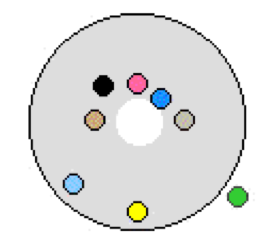
\includegraphics{figures/babble.png}
	\caption{Screenshot of Babble, showing high activity users (in the center) and lower activity users (around the edges), from \citep{Erickson:2003td}.}
	\label{fig:proxy-babble}
\end{marginfigure}

Although Erickson and Kellogg are particularly concerned with what is made visible and what is kept private (the difference between, in their terms, \emph{transparency} and \emph{translucence}), this is a point of divergence between our work. Although I agree with their analysis of the value of considering what actions should be made visible and what should be concealed, it is not a main focus of my analysis. In my work, reading is essentially always invisible and any other action is visible. This is partially a response to their suggestion that it is ``important that participants were aware of the others' awareness of [the properties of the system]'' \citep{Erickson:2003td}. This fits nicely with \citeapos{Brennan:1991wk} presentation of grounding. Simply being told something by someone is not enough for the conversation to move on - you must accept that presentation of information, and that acceptance needs to be accepted by the original presenter. In this way, grounding plays a role not just in communication itself, but in how we communicate information about who we are and what we're doing through actions in the system. 

This finding also suggests that if you don't know which actions are public and which are private, it diminishes the value of translucence as a design strategy. In their work, they tend to rely on physical metaphors to communicate the visibility properties of a system. This is a sensible strategy, but I feel this limits the kinds of experiences we can craft. In my work I tend towards not including invisible actions and instead create completely transparent spaces with carefully selected actions that are worth making visible. This is possible partly because the group sizes in my work are smaller than in the main examples they propose, and it's feasible to show all actions without it being overwhelming. 

\begin{marginfigure}
	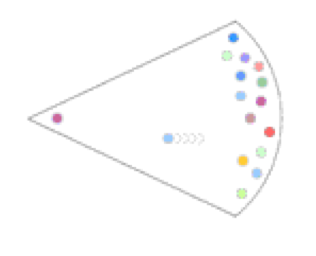
\includegraphics{figures/lecture.png}
	\caption{Screenshot of the lecture proxy, showing the speaker on the left, students on the right, and an interrupting student moving towards the left, from \citep{Erickson:2003td}.}
	\label{fig:proxy-lecture}
\end{marginfigure}

Erickson and Kellog a number of specific design findings that complement some of my experiences designing similar systems. They describe three approaches to visualizing activity: realist, mimetic, and abstract. \citep{Erickson:2003td}. I share their interest in abstracted representations, although for different reasons. They argue that realist and mimetic approaches face ``substantial pragmatic barriers (e.g. expense, infrastructure, support)''. In the years since this work was originally done (and well before; one might reasonably argue that \emph{ClearBoard} \citep{Ishii:1992bq} offered an elegant realist approach), many of those pragmatic barriers have fallen. We've seen large-scale virtual worlds (like \emph{Second Life}) that use mimetic approaches and wide adoption of video conferencing which uses realistic representations. I wish to argue that abstract representations are simply more flexible and better, even given the option of realistic or mimetic approaches.


My work goes into greater depth than Kellogg and Erickson's does on the issue of ``public not personal'' displays. While we agree that it is critical that each person's display doesn't deviate in the kinds of information it represents, in my work these displays are not monolithic---they are not the only venue for interaction between people. Furthermore, displays in my work are most often themselves public, which reinforces the grounding effect. Indeed, that is the most significant deviation between our work. In all of the social proxy work, the proxy is the primary communication medium; in my work, systems coexist with another primary communication channel, and rarely have any knowledge about the contents of that channel. Public displays also exacerbate issues of attention, which tend not to be major issues for work in the social proxy space (as shown in Table \ref{tab:related-work}). 

% put in a bunch of figures here of the social proxies they designed.



\begin{marginfigure}
	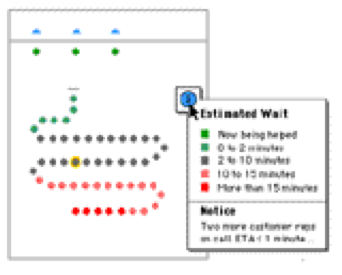
\includegraphics{figures/queue.png}
	\caption{Screenshot of the queue proxy, from \citep{Erickson:2003td}.}
	\label{fig:proxy-queue}
\end{marginfigure}

The other major distinction is in the use of metaphor and display techniques. Erickson and Kellogg limit their representations to ``a relatively large geometric shape with an inside and an outside and sometimes other features that represent the online situation or context'' \citep{Erickson:2003td} with ``small colored dots'' to represent individual users (similar to \citep{Viegas:1999kv}, minus the direct agency). These design strategies are illustrated in figures \ref{fig:proxy-babble} and \ref{fig:proxy-lecture}. Furthermore, they argue that the best way to represent information is through the use of ``relative movement'' of the user-dots in a way that has ``metaphoric correspondence to the position and movement of people's bodies in face-to-face analogs of the online situation.'' \citep{Erickson:2003td} As I hope my work shows, these limits are not at all necessary to create spaces of meaningful action that facilitate grounded communication and collaboration. Specifically, the need for relying on face-to-face analogs is not a helpful constraint. Instead, my work seeks to create spaces that are easily understood and provide contexts for meaningful action without relying on existing face-to-face metaphors.



\subsection{Channels}

\begin{marginfigure}
	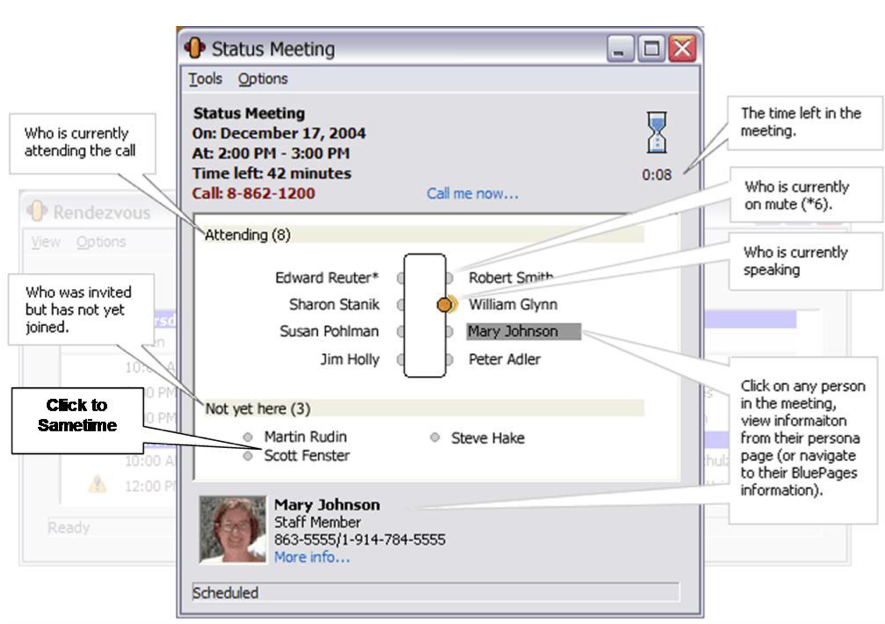
\includegraphics{figures/kellog_social_proxies.png}
	\caption{Screenshot of a meeting-room social proxy for promoting a sense of awareness of other meeting participants, from \citep{kellogg_leveraging_2006}.}
	\label{fig:social-proxies}
\end{marginfigure}

The primary focus of my work is on designing systems that add new communication channels and understanding how those channels operate in contrast to existing channels. In this section, I will present related work that addresses some of these questions.

\begin{marginfigure}
	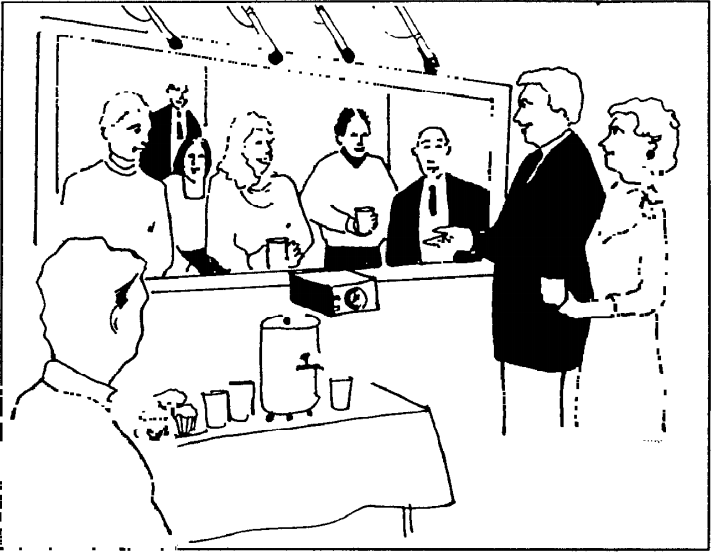
\includegraphics{figures/videowindow.png}
	\caption{Diagram of the VideoWindow scenario for connecting two work-place social spaces, from \citep{Fish:1990fn}}
	\label{fig:videowindow}
\end{marginfigure}

The work most directly related to these questions comes from research into so-called ``backchannels'' in presentation and classroom settings. \citet{Yardi:2006uk} describes how a chat-based backchannel operates over a semester in a classroom, \citet{mccarthy_digital_2004} describe a similar approach at a conference. Backchannels can also be considered a potential part of non-event-oriented contexts too, like long-term co-working among small groups. \citep{Huang:2003ef} Backchannels are not just focused on co-located groups, however, and \citet{kellogg_leveraging_2006} (among others, e.g.  \citep{Yankelovich:2005bx}) has addressed how text and audio backchannels can coexist in distributed contexts. Although past work has addressed in general terms the different ways people use backchannels, it has not sufficiently explained the complicated issues around channel selection, attention, distraction, and identity. Furthermore, in my work I try to move beyond just adding new text or audio channels by adding other kinds of non-verbal actions. In terms of my research themes, past work on backchannels has largely focused on characterizing use patterns, with some discussion of attention. More recent work, like \citep{Bergstrom:wl}, shares an interest in how we can construct actions and how shared displays can be used to help ground the interaction.

\begin{marginfigure}
	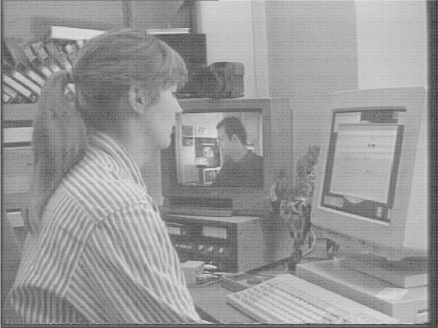
\includegraphics{figures/CRUISER.png}
	\caption{Photo of a CRUISER station installed in an office, from \citep{Fish:1992vz}.}
	\label{fig:cruiser}
\end{marginfigure}

\begin{marginfigure}
	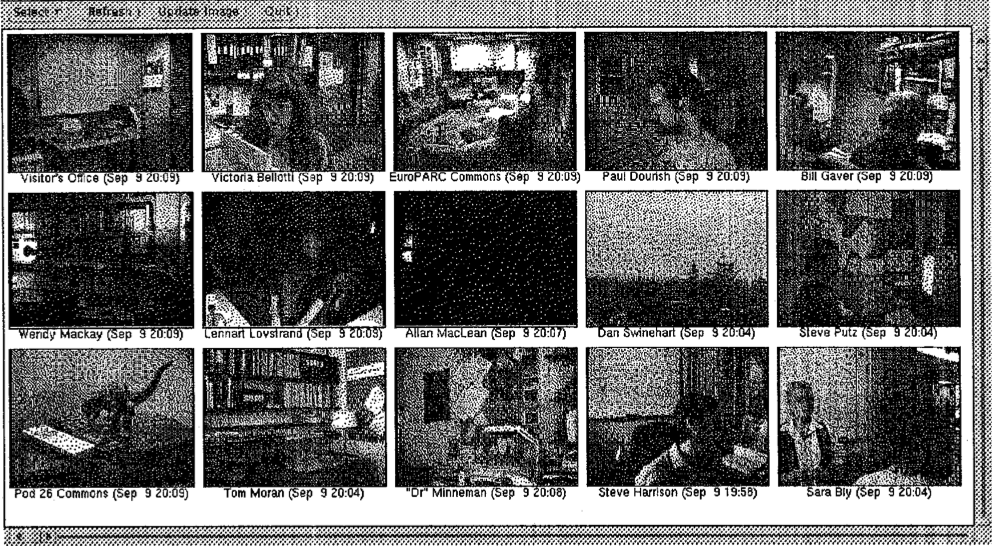
\includegraphics{figures/portholes.png}
	\caption{Screenshot of the Portholes interface, showing periodic stills from a wide range of environmental cameras in an office environment, from \citep{Dourish:1992fu}.}
	\label{fig:portholes}
\end{marginfigure}


Much of the work on creating shared media spaces, driven by experiments at PARC in the late 1980's and early 1990's is salient to my work. Although in some cases this work focused on creating new primary channels, researchers quickly became attuned to problems of privacy and attention because such systems always co-exist with face-to-face communication, in much the same way they do in the systems I design. The earliest work at PARC \citep{Olson:1991vz} focused on creating flexible video connections between offices and conference rooms. Subsequent work focused less on a phone-call-like model where connections are created and ended and shifted towards creating spaces with different affordances. Sometimes these involved connecting multiple individuals together, as in CAVECAT \citep{Mantei:1991ww}; other times researchers focused on creating long term persistent video connections in common areas of distributed research groups in the VideoWindow \citep{Fish:1990fn} project. 


Over time, attention shifted more towards taking advantage of the possibilities to do more than just create ``being there'' experiences. Some researchers experimented with audio-only spaces \citep{hindus1996thunderwire}, finding that video was not required to create a sense of connection and space for users, but that the properties of audio did require audio-specific etiquette and coping strategies for the system to be useful. iCom represented a particularly rich design perspective on connecting spaces  \citep{Agamanolis:2003wc}, recognizing that awareness need not be limited to visual awareness, but can extend to information awareness which can be productively embedded in a media space. This embodies the ``beyond being there'' model best of all the work in this research stream: not just trying to create a transparent window between remote spaces, but making something better than a window could be. Furthermore, these projects also focus more on issues of attention, because they are not necessarily always the primary interaction venue for their users. 

% \begin{marginfigure}
% 	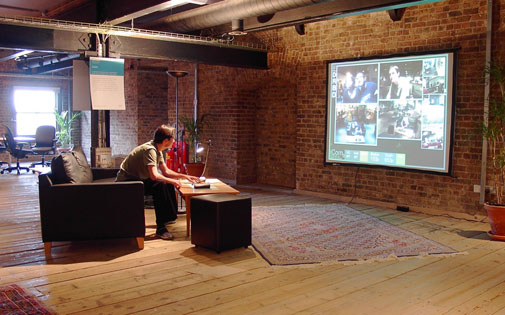
\includegraphics{figures/icom.jpg}
% 	\caption{Photo of one end of an iCom connection, showing multiple video streams and metadata along the bottom of the screen, from \citep{Agamanolis:2003wc}.}
% 	\label{fig:icom}
% \end{marginfigure}


\begin{marginfigure}
	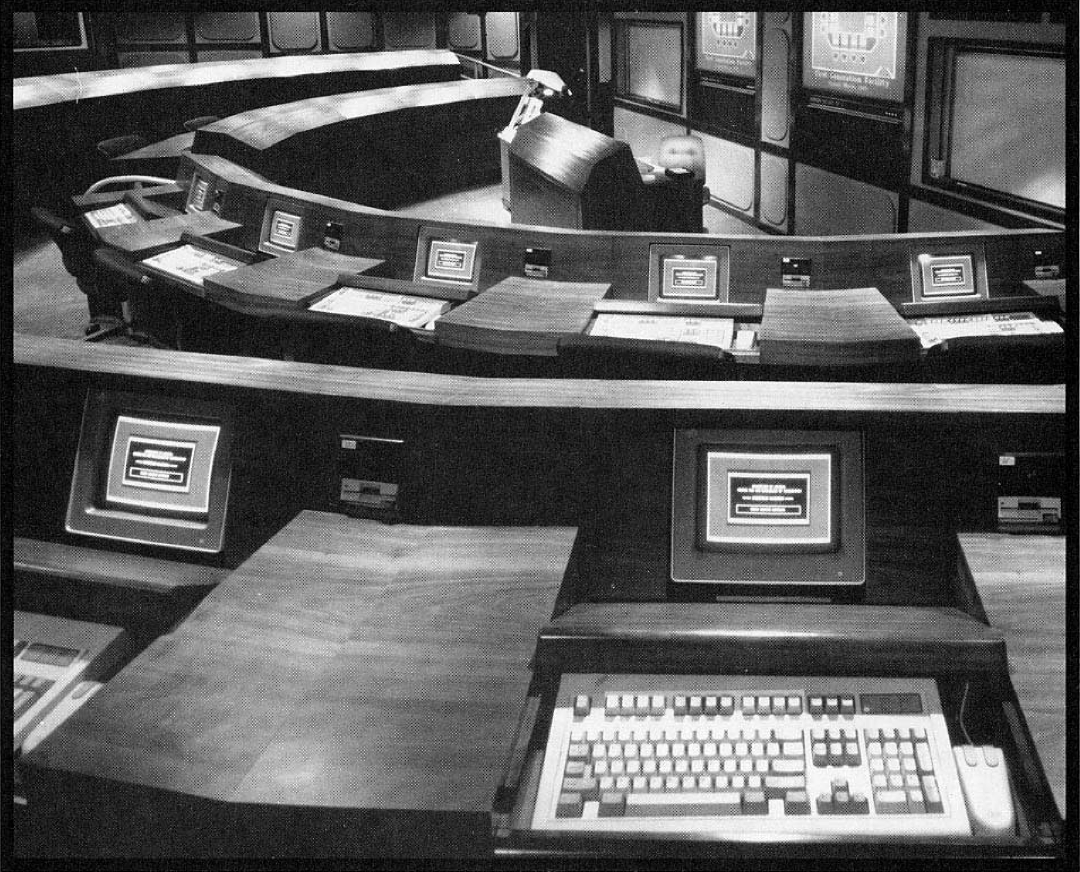
\includegraphics{figures/nunamaker_gdss.png}
	\caption{Photo of a GDSS space, from \citep{nunamaker_electronic_1991}.}
	\label{fig:gdss}
\end{marginfigure}


% also cite karrie's 
% (For subsequent, more artistically inclined approaches to this design space, see Karrie's blah blah, get a nice figure in here for that.)


Serendipity also evolved as an important part of sharing an office environment that was not present with most media space systems. Portholes \citep{Dourish:1992fu} addressed this explicitly by giving people a broader view of remote spaces instead of focusing just on main channel interactions. While my work is not concerned with serendipity, this kind of visual side channel carries important awareness information in much the same way that the side stages in my systems add important contextual information to an interaction. CRUISER \citep{Fish:1992vz} offered non-verbal ways to signal a desire to emulate some of the office hallway etiquette for signaling a desire to drop in and chat informally, without the explicitness of placing a call. The addition of moves like ``cruise'', ``glance'', and ``visit'' are similar in approach to the non-verbal actions at the core of my work like voting in \emph{backchan.nl}, promoting ideas in \emph{Tin Can Classroom}, or moving around the field in \emph{Information Spaces}. 

Early media space researchers proposed a distinction between ``formal'' systems and ``informal'' systems. \citep{Olson:1991vz} While most of the work discussed here (and much of my own work) tends towards the informal side of that continuum, there are some formal elements in my work. This formality manifests most strongly in Group Decision Support Systems research. These systems (exemplified by the work of Nunamaker \citep{nunamaker_electronic_1991}) provide prescriptive systems to support particular brainstorming, decision making, outlining, and voting schemes or policies. In the typical GDSS configuration, each participant has their own computer and interacts with shared structured data in some way, like submitting a new idea or voting on a proposal. In systems like this, the assumption is that having a structured display will ground otherwise informal processes by forcing participants to use the actions the system provides as a set of legitimate conversational moves. Although I tend towards informal systems in my work, the work in this space nonetheless has much to teach us about grounding and actions. 

The lack of consistent results in comparative work in this area \citep{Dennis:1988ww} illustrates the importance of focused design analysis to contextualize findings; it is not useful to view all brainstorming systems as equivalent and comparable in analysis, and I hope that my work will illustrate how the subtleties in interface and approach can have big impacts on outcomes that help explain some of the contradictory results in past GDSS work. Work in this space also raises serious questions related to attention that is largely unaddressed. In fact, in many situations the GDSS designers advocate for largely shutting down pre-existing primary communication channels to focus on the structured, mediated alternative.

Although somewhat rare in the literature, there are a handful of projects that directly address the kinds of hybrid spaces that I seek to create. \emph{Cognoter} \citep{Tatar:1991jq} addresses this design space most clearly. Like my work, \emph{Cognoter} created a hybrid space for very small groups (two to five people) that includes both personal and public displays where users can create items and spatially arrange them like on a whiteboard. Textual items can be arranged on a users' display and that arrangement is mirrored on all other users' personal displays. The authors characterize \emph{Cognoter}'s model of creating shared text elements as representing a ``parcel-post'' as opposed to an ``interactive'' conversational model. Instead of embodying a present/accept process (as described by \citep{Clark:1989uc}), they describe their process as being more like literary communication (such as email) where the writer tries to make sure ``that the addressees \emph{should have been able} to understand his meaning in the last utterance'' (emphasis mine). This is in contrast to face-to-face interaction, where we can interactively ascertain the extent to which we are being understood (and repair mistakes) before moving on. The authors describe \emph{Cognoter}'s failure to be used effectively by its users as (in part) a conflict between the interactive mode of face-to-face communication and the parcel-post model in \emph{Cognoter}. The \emph{Thoughtswap} project \citep{DickeyKurdziolek:2010wt} also shares the goal of creating a complementary communication system. Like \emph{Cognoter}, the mediated space is used serially with the face-to-face space, while I am interested in creating spaces for legitimate simultaneous performances in mediated and non-mediated spaces. This suggests a major hurdle for my work: can we create systems that use a parcel-post model yet still integrate fluidly with the interactive face-to-face model? \emph{Cognoter} and \emph{Thoughtswap} suggest this is hard, but I will show throughout my work how these barriers can be overcome and suggest ways to explain \emph{Cognoter}'s negative findings.

% go hunting for a desanctis and/or poole piece that's not focusing on AST specifically? also can hit berg if we want, but it feels like a bit of a distraction at the moment.

%, they also produced a nice taxonomy of the kinds of tools that would be useful for distributed collaborative groups: synchronous versus asynchronous communication and open processes versus focused processes, a distinction 


% there's a funny note in the portland paper about how they want to shift away from meeting augmentation to async and task coordination. Funny how times change.

% now summarize. 


% going to want to bring up media equation or whatever that book is called. Cliff Nass. 




% thundewire is just audio, basically a single-channel mumble. not so much about results as describing practices that evolved. 
% portholes is ambient awareness about remote places, not live interaction. cut it?
% videowindow is just like hole in space - audio/video fixed in space

% also mention virtual world stuff? MASSIVE might be worth a quick ref

% "shared media systems"

% - video projects like thunderwire + portholes
% - videowindow


% organize the work in this space 
% projects to talk about:
% - voiceloops
% - backchannel literature
% - social proxies
% - mention conferencing apps
% - Nunamaker
% - zephyr?


% \subsection{Theoretical Perspectives}
% thinking about leaving this out

% stuff from cscw paper:
% systems for reflection
% - second messenger
% - "social mirror" (Karahalios) also bergstrom
% - Meeting Mediator
% 
% systems adding new channels
% - (all the backchan literature: yardi, mccarthy, huang, kellog, yankelovich)
% - do a section on nunameker's work and why it's weird
% - 

% - we'll want to at the very least nod to thinks like voiceloops, and all the audio/video stuff like portholes and thunderwire and that kind of thing. farm my generals reading for that part.
%


% theoretical perspectives
% - practice lens?
% - ethnomethodology? 
% - re-farm wanda's reading list to see what else I can pull from there.

%
% We'll need to do a little organization here. Obviously, farm the references from the Tin Can Edu CSCW paper + backchan.nl paper. We'll need more, ofc, but it's a start. I suspect there will be some ways to separate out systems that allow communication versus those that simply reflect on a main channel. Maybe it's about whether the system itself is a single channel, multi channel, main channel or side channel? 

% write a methodological section here about why it's useful to study this with design work

\subsection{Reflection}

\begin{marginfigure}
	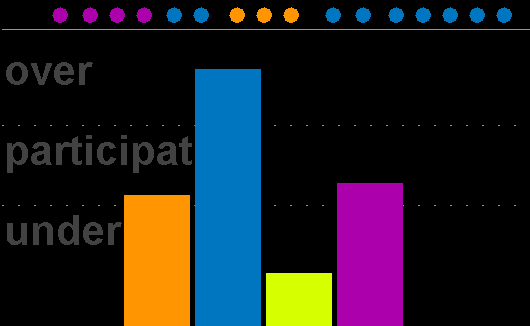
\includegraphics{figures/second-messenger.png}
	\caption{Screenshot of a Second Messenger participation bar-chart, from \citep{DiMicco:2007ie}.}
	\label{fig:second-messenger}
\end{marginfigure}

% \begin{marginfigure}
% 	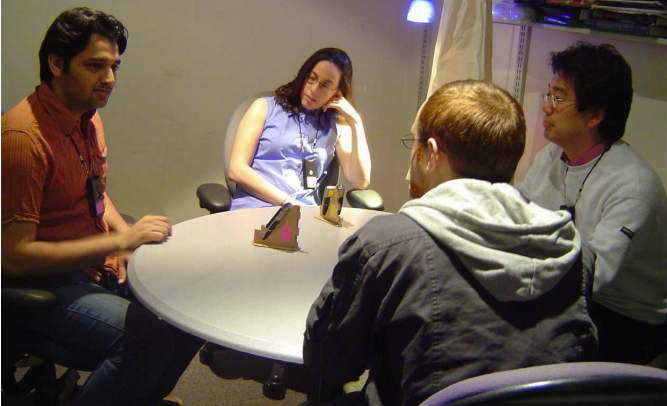
\includegraphics{figures/meeting_mediator.png}
% 	\caption{Meeting mediator.}
% 	\label{fig:meeting-mediator}
% \end{marginfigure}




Understanding how we present ourselves to others has been a topic of sociological inquiry for quite some time. Although many of the insights of scholars like \citet{goffman_presentation_1959} about how we communicate and interpret information about who we are and how we want to be treated are still relevant, the information that is available about people has changed substantially. In some of the examples in this section, designers have added some new bit of information about people to a face to face discussion; in others, we don't have any of the traditional information we would get from being face to face with someone and rely on new types of signals (like the non-verbal actions I propose) to create a sense of people around us. Part of what sets mediated communication apart is the ability to accumulate behavioral histories and represent and reflect those histories to ourselves and others. The work in this space is not as closely connected to my main research themes, but I include it here primarily because it has served as a source of design inspiration. 


\begin{marginfigure}
	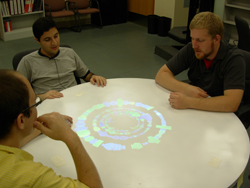
\includegraphics{figures/conversation_clock.png}
	\caption{Photo of Conversation Clock in use, showing relative participation histories from each conversation participant, from \citep{Bergstrom:2007je}.}
	\label{fig:conversation-clock}
\end{marginfigure}

My work is substantially inspired by the work of \citet{DiMicco:2007ie} on the \emph{Second Messenger} project. In this project, participants in a group discussion were presented with a constantly-updating bar-chart visualization representing the relative amount of time they had talked during the discussion. They found that while people who over-participated without a visualization tended to moderate their participation when the visualization was present, people with low participation did not participate more just because others were participating less. \emph{Meeting Mediator} \citep{Kim:2008ip} took a similar approach, but focused on situations where groups of two people could see each other and had to interact with another group of two people that they could only hear. Using a different visualization, Kim et al. found that groups were more interactive with the system than without, although there was not a correlation with group performance. 

\begin{marginfigure}
	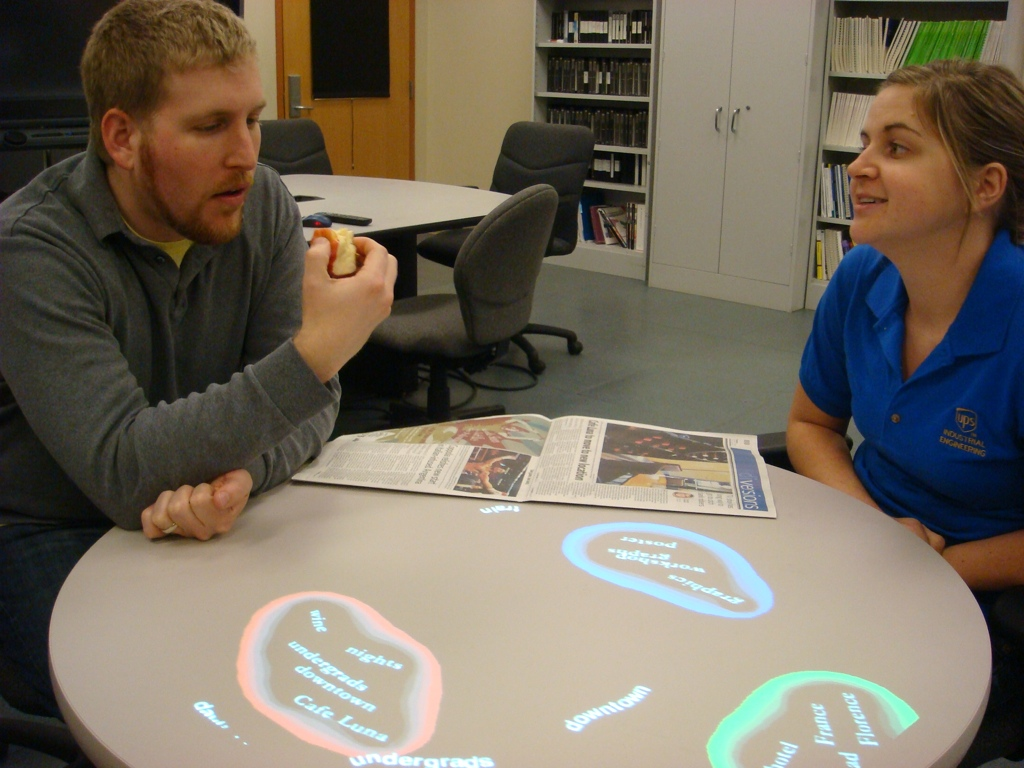
\includegraphics{figures/conversation_clusters.jpg}
	\caption{Photo of \emph{Conversation Clusters}, detecting audio themes and displaying them in visual clusters on the table-top display, from  \citep{Bergstrom:2009fe}.}
	\label{fig:conversation-clusters}
\end{marginfigure}


Bergstrom has done a series of projects that adopt a similar design strategy. \emph{Conversation Clusters} \citep{Bergstrom:2009fe} pulls topics from an audio conversation and presents them in clusters on a table-top display. \emph{Conversation Clock} \citep{Bergstrom:2007je}, like \emph{Second Messenger} and \emph{Meeting Mediator}, visualizes conversation participation, but uses a timeline metaphor instead of an aggregative metaphor. \emph{Conversation Votes} \citep{Bergstrom:2009ej} lets uses discreetly vote about the progress of a discussion, and displays anonymous votes on a table-based display. \citet{Karahalios:hu} describes this design space as ``social mirrors''. 

\begin{marginfigure}
	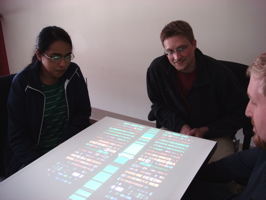
\includegraphics{figures/conversation_votes.jpg}
	\caption{Photo of \emph{Conversation Votes}, showing voting history among conversation participants on the table-top display, from \citep{Bergstrom:2009ej}.}
	\label{fig:conversation-votes}
\end{marginfigure}


% sneak in a \citep{visiphone} here?


% MATT TODO FIX THE MIDDLE OF THIS PARAGRAPH IT'S AWFUL
These are all examples of the accumulate and reflect design strategy, where the system tracks some aspect of behavior: spoken participation in the case of \emph{Second Messenger} and \emph{Meeting Mediator}, discussion topics and group attitudes in the case of Bergstrom's work. 

%The systems then present that information back to the individual or group with the intention that to reflect on and adjust their behavior. Furthermore, all of these projects have an element of grounding to them. By presenting this social information on a shared display (as in my work), it is made salient to the discussion in a way that private displays cannot.

% cite things like last.fm, goodreads, etc in this space?


% \subsection{Identity}

% maybe this whole section is dumb.
% how often do I really deal with this? It's clearly part of the second life work, but not at all part of backchannl, and only a little a part of the Tin Can series. Erm. Move on for now and double back. 

% Many other projects have focused on how peoples' identities are presented. In most of these pieces, there is no face-to-face element, which drives the researcher's interest in developing compelling alternative options that can richly communicate who someone is in a mediated space. Many informal and practical options are in common use; displaying an icon or image chosen by someone and a pseudonym to represent themselves is a widely used design strategy in social applications throughout the internet. These spaces for self expression are frequently augmented by systems that aggregate someone's behavior in that space. This is much like the reflection techniques, but are usually summarizing events beyond any single person's experience. The community site StackOverflow \citep{stack_overflow} provides a particularly rich example of this strategy.

% screenshot a wow forum, stackoverflow, 

% These techniques feel thin compared to the richness of face-to-face interaction, and researchers have developed a number of alternative approaches. Donath's work on data portraiture in a variety of 



% link to things like Ros' work in terms of augmenting face to face interaction with extra information? Or go back to steve mann's cyborg stuff?

% need a paragraph here that's more about the identity side of things. not sure what that will be. chat circles, perhaps? talking in circles? (whichever one had that intersting voting shapes thing)

% how to fit in social proxies and social translucense



% Other potential bits we could fill in here...
% We could spend some time with social translucense
% We could look at non-vebal actions as a space
%	start with Greenbergs stuff, but really look all over for groupware/collaborative tools that had some action to them. Will find some of that in the CVE literature, which might be easy to find
% I don't talk at all about theory stuff here. Could do the spiel about shared displays and grounding, but I'm not sure how critical that is going to be ultimately.
%
%
%  One other strategy is to think about the three research themes: grounding, non-verbal actions, and attention, and go on a hunt for good literature about each of those. 


\subsection{Meeting Structure}

Any system designed to support interaction makes a number of implicit assumptions about the nature of the social process it's trying to support. This is true across design domains. For instance, calendaring systems often assume that the important aspects of someone's work life can be captured in meetings. Meetings have a time, a place, and other meeting participants. Certainly, this describes some kinds of work life, but plenty of other jobs don't fit with that metaphorical structure. Imagine a car repair shop; a system to support that sort of work environment would necessarily be concerned with specific tasks that need to be done and which people in the shop were going to do them. A meeting organization system would not be as appropriate for managing that environment. Of course, over time systems influence people's behavior in such a way that it makes it hard to distinguish between the implicit assumptions about how people would use the system and how their behavior has adjusted to best make use of the systems they have available. 

Meetings are rich social experiences that are composed of a variety of deeply interconnected components. I turn to \citeapos{McGrath:1984un} theoretical framework as a good starting place for understanding the diversity of factors that influence a group's process. McGrath describes groups as ``task performance systems'', recognizing the critical extent to which tasks characterize a group's interaction, along with the group composition, the properties of the environment, and properties of the individual. He identifies eight types of tasks: planning, creativity, intellective, decision-making, cognitive conflict, mixed-motive, competitive, and performance. In this chapter we are primarily concerned with decision-making tasks.

Various structures for organizing decision-making have been proposed. One interesting structure is IBIS \citep{Kunz:1970wo}, which classifies the structure of arguments in design meetings. In their model, a discussion has Issues (e.g. ``Users aren't using this feature as much as we thought they would''), Positions (``We should include the feature in our tutorial'') and Arguments (``Not many users are following the tutorial either, we need another way to promote this feature.''). These objects are linked by different relationships, like ``supports'', ``objects-to'', ``responds-to'' or ``specializes''. This creates an abstract argument network that organizes the discussion around concrete issues. \citet{Conklin:1988fr} describe a computer-supported system that uses this structure for both synchronous and asynchronous discussions. This basic approach of modeling a particular task network in a formal way is shared by many Group Decision Support Systems of which \citet{nunamaker_electronic_1991} is a nice overview.

In McGrath's terms, though, systems like gIBIS (and many of the systems described in the GDSS literature) are not strictly addressing one task. They're nominally about making decisions, but a group using gIBIS is also sometimes trying to solve intellective tasks (e.g. solving questions with a single right answer), perform generative tasks, and perhaps resolving conflict tasks. The precise mix of these tasks varies in each group's process, which creates a significant diversity in system designs. Structures that assume a particular task profile are unlikely to be effective when applied to another task profile.

Task profiles are one example of a formalizing instinct to organize and abstract certain features of human practice in a way that can help us both better understand those practices or (in the case of designers) design tools that support those practices. Not only is it a question of useful or accurate abstractions, it is also a tension between the right amount of structure and too much structure. A model like IBIS or Roberts' Rules of Order \citep{RobertIII:2000tq} is relatively heavy amount of structure. In contrast, process models like nominal group technique \citep{Bartunek:1984cq} operate at an even higher level of abstraction. In general, my instincts lean towards less formality rather than more, but that reflects the sorts of practices I'm creating tools for more than a real argument for either strategy. Regardless of how one decides to abstract, there is still a complex relationship between the selected formalism and the practice it is either modeling or seeking to promote. \citet{Berg:1997bs} describes this interplay this way:

\begin{quotation}
By offering abstracted models of the work and/or by processing input into output, formal tools are attributed central roles in organizing the work within the workplace.
\end{quotation}

Berg organizes the camps on this issue into two main discourses: naive formalists who believe that formal models are necessary for rational or scientific decision-making and scholars who argue that the texture of human practice defies reduction to formal models. This argument has a political angle to it, as well, arguing that (as Berg describes it) formal tools will ``inevitably function in a rigid, impoverished way, thus de-skilling and dehumanizing the work of those who are caught in its cold, instrumental rationality.'' These are both extreme views and not widely held at this point. Berg characterizes the distinction between the formal tool and the human practice as being like the distinction between the map and the terrain it describes. Maps are a way of abstracting and describing terrain, while also influencing the ways that people understand and develop that terrain. They are necessarily tightly interrelated.

Although Berg is primarily interested in building theoretical tools for better understanding practices at the boundary between formal tools and human practices, this perspective is also valuable for designers. Formal model building is a critical step in designing any sort of software system. Indeed, designing abstract representational models for data is a core part of any software design process. \sidenote{\citet{Hughes:tv} is a clever (if somewhat inaccessible to non-database engineers) analysis of the challenges representing human marriage practices in a database. It illustrates, too, the built in biases of computational systems towards certain sorts of convenient abstractions despite their lack of grounding in practical experience.} As researchers we frequently have our own agendas and are trying to describe future terrains that may not exist yet. Put another way, maps are sometimes guides to exciting new terrain, not just describing a certain perspective on existing terrain. This is more precisely the sort of work that I do.

In the chapters that follow, I will describe a series of projects. For each of these projects, I will attempt to identify the existing practices it seeks to support, as well as the sorts of new practices it aims to encourage through the formalizing effects of software systems.


% Another model with a task profile more focused on resolving conflicting viewpoints is the Public Conversations Project \citep{PublicConversations:ta} uses a system for having dialog about controversial issues (e.g. Israel/Palestine, reproductive rights, etc.) that focuses on the context and structure of the meeting. These meetings are intentionally not about reaching consensus, but instead about building understanding, which makes an argument-based structure like IBIS inappropriate.
% 
% 
% Part of what's exciting about working in virtual worlds is that the basic rules of a space don't preclude lots of different kinds of interfaces being built within it. The system I propose in this chapter is a simple model (neither IBIS or the PCP models) that is appropriate for only certain kinds of meetings. I imagine it as being one of eventually a set of spaces designed to work for specific situations. Just as a company might choose to use IBIS for some of its meetings, a meeting moderator in a virtual world can choose to use this space or some other virtual space for their meeting depending on whether or not their needs and the structure of their interactions are a good fit for the space.

\chapter{Virtual Spaces}


Over the past twenty years, the prospect of visiting a virtual world different from our own world has moved from being strictly the domain of imagination to being widely accessible. What started as worlds accessed through typed commands and presented as text have evolved into rich graphical and sensorial experiences that became rapidly accessible to mass audiences. The argument for virtual worlds has always had a revolutionary tone. Virtual worlds might, for example, suppress the prejudices of offline society by hiding identity information, breaking down the boundaries of distance, and making experiences broadly accessible that might not otherwise be feasible. Perhaps we could even build a new virtual society, one that is better than our own. These utopian visions are attractive precisely because the urge to grow beyond the confines of everyday experience is so strong.

This vision was so attractive that in the mid 2000's the market research firm Gartner famously predicted in 2007 that by the end of 2011, ``80 percent of active Internet users (and Fortune 500 enterprises) will have a `second life', but not necessarily in \emph{Second Life}.'' \citep{Anonymous:2007wz}. This has not come to pass. Linden Lab has stopped publishing public usage data, but it is clear by comparing its cultural impact to systems like \emph{Facebook}, \emph{Twitter}, and \emph{YouTube} that \emph{Second Life} has been almost completely eclipsed in the public imagination by other types of mediated social experiences. Despite this shift, it is still productive to attend to this period where virtual worlds were viewed as strong potential venues for mediated social interaction. What attracted us to these experiences in the first place? Why did these experiences ultimately fail to catch people's imaginations? Are there aspects of ``virtual'' experiences that were left behind in the shift away from a ``virtual'' approach that might be valuable components of more modern experiences? Why did the reality of accessible virtual worlds fail to live up to their revolutionary, utopian promise?

In this chapter I will address these questions through an analysis of the properties of virtuality and a pair of design projects: \emph{Information Spaces} and \emph{Presentation Spaces}. Although these projects do not exemplify the best sorts of \emph{in situ} research, they serve as conceptual arguments about how we might think about designing virtual experiences that take advantage of what virtuality offers designers that is missing in other approaches to mediated interaction. This is in contrast to much of the design work in virtual worlds in this period that focused instead on replicating the forms of offline experiences and expecting them to have the same properties when transplanted into a virtual context.

Although in its specifics this argument is perhaps a little dated and unlikely to apply directly in the future (barring a resurgence of virtual world design), it can be seen also as an argument for how to do a close reading of the properties of a platform and letting those properties guide a design that is closely adapted to its tools. Considering virtual worlds in this detail helps highlight some of the taken-for-granted assumptions about non-virtual design.

In a larger sense, a deep discussion of virtuality will also demonstrate how the core research themes of this thesis--grounding, non-verbal actions, and attention--operate in an unfamiliar context. Although readers might be unfamiliar with operating in a virtual world environment, this unfamiliarity will help address these research themes without preconceptions.

I open this chapter with a discussion of what precisely defines a ``virtual world'', focusing on the distinction between spatiality and dimensionality. 


% TODO this isn't actually how I open, fix this.




I will defer an analysis of why this might have happened for later in this chapter, but 


As with many technology trends, there is a sort of pendulum that swings between different design strategies. Our earliest mediated social experiences (like email and chat) were primarily text-based media. 



This chapter explores some of my early work in the virtual world space and draw comparisons between 


\section{Characterizing Virtual Worlds}

Although there is no single definitive typology of virtual worlds (though there are many examples, e.g. \citep{Koster:2007wg}), there are a few general categories that are important to properly describe the kind of worlds that this thesis is concerned with.

The two major axes on which virtual worlds can be organized (as proposed by \citet{Bartle:2003up} are agency (which Bartle calls `change') and persistence. Agency is a broad term that is the set of things that someone can do in a world. Agency can be thought of as the interface that you have onto the world. For example, the agency of players in a chess game is limited. When it’s their turn they can move their own pieces in certain prescribed ways. Moving pieces is the agency players have in the chess game. In virtual worlds, agency becomes a bit more elaborate and includes movement, avatar customization, communication, object creation, etc. Different worlds have different sets of actions that an avatar can do, and I describe them as having different kinds of agency.

Persistence is the ability of the world to remember events that change something about the world. For example, if you create an object in a persistent virtual world you can expect that the object will be there when you return. This is in contrast to worlds where changes aren’t saved for very long. Multiplayer first person shooter games are a good example of this---you interact with a rich three-dimensional world and might change it by dropping weapons, causing explosions that change the appearance of part of it, or by destroying certain objects in the environment. None of those changes will remain in that world the next time you play, though. It will be wiped clean and you’ll have a fresh copy of the original space. These spaces often even revert to their original state after a few minutes: bodies disappear, dropped weapons fade, and explosion marks are removed. 

Certainly, these axes are not perfectly distinct (worlds with limited agency often have low persistence as well), but they serve as good organizing principles. For the most part, modern virtual worlds have high levels of agency but relatively low levels of persistence. In \emph{World of Warcraft} for instance, players can kill monsters in the world, but the monsters will always reappear a few minutes later. There are virtually no actions players can take that modify any aspect of the world apart from killing computer controlled characters. Rich agency exists almost entirely in the relationships between players and the organizations they form. Worlds like this have proven to be commercial successes because they are more resistant to disruptive behavior aimed at degrading other players' experiences, but they also rule out many of the interesting opportunities that virtual spaces offer over physical spaces.

The best recent example of a world that offers that kind of rich agency and persistence is \emph{Second Life}, a world developed by Linden Lab. \emph{Second Life} is a free application that connects to a single monolithic ``Grid'' of \emph{Second Life} servers that provide a mostly continuous (flat) virtual space in which avatars can own land and items, build clothing, buildings, or vehicles, and embed behavioral scripts in their creations. The world also provides an economic system with its own currency system (the Linden Dollar, L\$), which is exchangeable at a fixed rate for US Dollars on a currency exchange that Linden Lab manages. The community that has arisen around \emph{Second Life} is extraordinarily diverse and rich, but an in depth discussion of its dynamics is beyond the scope of this chapter. There are a number of books that describe the history and culture of \emph{Second Life}, which provide a good introduction to that topic, however. \citep{Au:2008va, Ludlow:2007uu} For my purposes, \emph{Second Life} is critical as an example of a world in which avatars have a considerable amount of control over the design of environments, and so \emph{Second Life} has been instrumental in developing an intuition for how virtual spaces influence the behavior of people in them. It has also been useful as a platform for exploring the design space of algorithmic architecture. For much of this chapter, I will turn to \emph{Second Life} as a source of inspiration, as well as to draw comparisons between the general model for virtual architecture that I explore in this thesis and the model that \emph{Second Life} embodies.

\subsection{Representation and Function}
Specific features of both physical spaces and virtual spaces can be thought of as serving symbolic and functional purposes. As virtual spaces were first being conceived it was not obvious that they would draw their symbolism heavily from physical spaces \citep{Novak:1991ue}. Novak would no doubt be surprised to see how familiar the design elements of can be. In the free-form world \emph{Second Life}, for instance, there are countless recreations of both specific architectural landmarks as well as buildings that ape familiar architectural styles. Furthermore, those buildings are filled with rooms furnished in a way that would not stand out in the least from their real world analogs. Why is it that, free of the natural laws of the physical world, so much of virtual world design is concerned with recreating familiar physical spaces?

This focus on familiar representations serves a number of important social roles. First, it functions much like the identity signals do in physical fashions. Although choosing and furnishing a virtual house is substantially less costly than its physical analog, it is still a strong demonstration of taste that helps visitors to virtual spaces understand something about the person who assembled them, much like a personal homepage or profile page might on the Web. And though the price of virtual items may be substantially less than the physical artifact it mimics, virtual economies usually have some sense of relative value that allow these items to also function as signals of wealth.

The second important social role is in building spaces that contextualize behavior. Visitors to virtual worlds are forced to reform their notions of socially acceptable behavior in virtual spaces. It is substantially easier to make meaning from a virtual space built to look like something familiar than something abstract. In this way, avatars in virtual spaces can reasonably expect that spaces that look like virtual museums, dance clubs, meeting rooms or houses should be used for virtual analogs of what one might do in their offline equivalent. This argument is analogous to Norman’s, with respect to the design of interactions with physical objects \citep{Norman:2002tv}. He describes how physical objects use metaphors to demonstrate affordances. Metaphors imply a conceptual model that makes it easier for people to make deductions about what how their interactions with the system will affect it. In a very similar way, literal representations in virtual architecture serve as behavioral affordances. They use architectural metaphors to imply what the social model of the space should be. 

Although literal representational techniques serve effectively as identity signals and behavioral affordances, this does not mean that they are the only way to do effective design work in virtual worlds. Indeed, the work in this chapter will try to demonstrate an alternate approach.

I will describe spaces which not just look different and imply that different behaviors are expected but spaces that actually have different functional affordances that make certain activities more or less effective in a particular space. Functional affordances are those that are not simply based on what the space looks like, but what aspects of the world that are algorithmic and reactive in some way. We should treat virtual space as a new medium that has its own strengths and weaknesses instead of trying to create the experience of ``being there.'' This distinction is best understood through analogy to how symbolism and function interplay in two kinds of physical spaces: cathedrals and nightclubs.

The form of a classical cathedral is rich with religious symbolism that informs the overall structure of the building, detailed adornments, lighting, and scale. It also has certain functional affordances. The space is designed such that a speaker at the podium can be easily seen and heard by the people in the pews. This also means that the whole congregation will easily hear any noises from the pews. This encourages parishioners to be quiet, and re-enforces the power dynamics inherent to the church; visitors are not there to interact with each other.

Nightclubs use acoustics and lighting to create a very different kind of space. Although the precise form of clubs varies, the functional aspects of clubs are often quite similar. Loud music makes it hard to hear people far away, which both forces people to be close together to talk and makes it hard to be overheard. In this environment, it is easy to have intimate conversations. Low lighting makes it difficult to see people, hear them, and identify them. This creates a situation in which people must fill in information about each other because the environment makes that information hard to get. Darkness and candlelight in a cathedral would have a different effect---the functional and cultural/symbolic meanings are interwoven.  The nightclub is known to be about hedonism and escape; the cathedral, for the believer, about spiritual, solemn, and perhaps frightening/awe-inspiring experience.

Lighting and acoustics are two aspects of what I call ``functional'' aspects of space. They operate mostly independently of how a space looks (that is to say two spaces could look the same but have different acoustics) and both respond to people’s actions in the space as well as mold those actions. These two examples demonstrate how the functional side of spaces has a big impact on what kind of activities make sense in them. You would not, for instance, try to hold a business meeting in a nightclub or hold small group discussions in a cathedral. Yet virtual spaces very rarely have this kind of adaptability to their designed purposes. You could, in a world like \emph{Second Life}  hold a business meeting in a virtual night club with no particular ill effects. It would be a strange juxtaposition, but the location would be only a visual distraction, not a major impediment to having a conversation. The heart of this chapter is to show how building virtual spaces that exhibit some of these same sorts of properties might create compelling virtual experiences that are competitive with non-virtual interfaces.

\subsection{Dimensionality and Spatiality}

It's difficult to pin down exactly what makes a virtual world a world. In the previous section we draw the distinctions of agency and persistence from the literature. These are useful for distinguishing between different sorts of world, but are not sufficient to distinguish worlds from non-worlds. Another attractive potential to draw a distinction between worlds and non-worlds might be a certain immersive representation. When we think about immersion, we typically presume that means a three dimensional representation. 

\begin{quotation}
One question we are frequently asked is why use 3D for a collaboration environment? While it might be possible to build a 2D tool with functionality similar to MPK20, the spatial layout of the 3D world coupled with the immersive audio provides strong cognitive cues that enhance collaboration. For example, the juxtaposition of avatars in the world coupled with the volume and location of the voices allows people to intuit who they can talk to at any given time. The 3D space provides a natural way to organize multiple, simultaneous conversations. Likewise, the arrangement of the objects within the space provides conversational context. If other avatars are gathering near the entrance to a virtual conference room, it is a good guess that they are about to attend a meeting in that space. It is then natural to talk to those people about the content or timing of the meeting, just as you would if attending a physical meeting. In terms of data sharing, looking at objects together is a natural activity. With the 3D spatial cues, each person can get an immediate sense of what the other collaborators can and cannot see.\citep{Anonymous:tv}
\end{quotation}


The role of dimensionality in virtual worlds is subtle. Like the authors of Wonderland (neé MPK20), I am often asked about the tradeoffs between working in two dimensions versus three. To answer this question, I think it’s important to tease out the difference between dimensionality and spatiality.

The dimensionality of a world is an aspect both of its display and its abstract data representation. Objects in a three-dimensional world have a position in three-dimensional space, a solid volume, and an orientation in three rotational axes. In an intuitive sense, a three-dimensional virtual world looks a lot like the three-dimensional physical world we are used to. The programmatic representation of the world need not be bound to its visual representation, however. It is possible to build a three-dimensional representation of a fundamentally two-dimensional world. The MASSIVE system demonstrates this nicely; they had both a three-dimensional visual client and a text based two-dimensional client. Both clients could almost completely represent the world state. As a world, MASSIVE had no vertical dimension, so its three-dimensional representation was simply a skin on a two dimensional world. \citep{Greenhalgh:1995gz} What’s important, though, is drawing a distinction between the dimensionality of the world itself and the dimensionality of its visual representation—they need not necessarily be the same thing.

The perspective on a world is an important related aspect of the world that is related to its dimensionality. Three-dimensional worlds have two major perspective options: first person and third person. In a first person perspective, the user views the world as if the camera was placed where the eyes of the avatar would be. If they see their own body at all, it is usually only their hands or feet. In this mode, the user literally inhabits the body of avatar and becomes that character in a significant way. In a third person perspective, the user sees their character from a camera that is usually behind them looking down. This provides a better sense of the world around their character, but can sacrifice some immersion by showing the avatar animating itself or looking different than a user’s own vision of them. The choice of perspective is primarily one of immersion: first person views are more immersive than third person views. In two-dimensional worlds, third person views are essentially the only option. A first-person two-dimensional view would be Flatland \citep{Abbot:1899th}, with all of the challenges of navigation and interaction explored in that book.

Spatiality is harder to precisely describe because almost without exception virtual worlds are all spatial in some way or another. MUDs offer perhaps the best starting point as one of the least spatial examples of a virtual world. In a MUD, players occupy discrete rooms. Each room can contain many players and objects, and is connected to other rooms through a series of nominally spatial relationships. For instance, from a given room, you might direct your character to move north which would move your character into the room that the system thinks is north of the room you were in. Although this model is spatial in the sense that you can be closer or farther from people, avatars in early MUDs had little agency or perception of events anywhere but their current room. In a given room, there is no functional spatiality; all players and objects occupy a sort of indistinct space where they could hear and interact with each other, but have no finer position than the room itself. As a result, there was no context for using the kinds of spatial language that make spatiality so useful. A player couldn't describe an object as being ``the thing on your right.''

Furthermore, the connections between rooms themselves were not reliably spatial in any particular way. Although they were ostensibly arranged in cardinal directions, there is no enforcement of “normal” spatiality. A series of rooms could easily fold back on itself such that moving north a few times would return you to the room you started in. Different routes out of a single room might all go to the same room. Paths might even behave differently in different directions; moving north from one room to another, and then south to try to get back again might not necessarily take you back to where you started. In this way, even an ostensibly spatial metaphor breaks down and fails to convey the contextual and perceptual benefits of true spatiality. In contrast, a world where objects and avatars have distinct discrete locations immediately confers these benefits. Avatars can indicate group membership by avatar proximity, can have a shared visual reference point, and so can communicate about objects behind or to the right of other avatars. 

Returning to the quote about MPK20 that introduced this section, I argue that they are conflating notions of dimensionality with spatiality. All of the beneficial features that are ascribed to a “3D world” are more properly ascribed to a world with rich spatiality. A two-dimensional virtual conference room can have an entrance where avatars congregate just as easily as a three-dimensional world. Two-dimensional worlds confer the same benefits regarding shared gaze, too. An avatar in a two dimensional world can infer another avatar’s view on that world in the same way they might in a three-dimensional world. These are all properties of a world’s spatiality and not its dimensionality. Although the work I describe in this chapter is two dimensional, I have maintained spatiality wherever possible. This maintains many of the benefits in the introductory quote while avoiding the many challenges of working in three dimensions. Translating this design approach into three dimensions is certainly possible, although maintaining spatiality in three dimensions requires a certain vigilance. \emph{Second Life} is an instructive example here. Avatars in \emph{Second Life} freely move their cameras with no external representation of its current location. As a result, an avatar’s position in the space has little to do with their current view, and so spatial language isn’t necessarily that useful.  Chapter 4 demonstrates how three-dimensional spaces can be used with this same approach, and similar analogs could be built for essentially all the zones and ideas presented here.

While I believe that worlds that are fundamentally two-dimensional are not inherently less spatial than their three-dimensional counterparts, there is something to be said for the representational language (as opposed to the functional or algorithmic language) of three-dimensional spaces. As discussed in the previous section, three-dimensional spaces tend to offer more legible spaces because they use a representational language that is familiar. Meeting rooms represented in three dimensions (or even some sort of isometric view) may be more obviously meeting rooms than the very abstract vector-graphics style rooms I show in this chapter. For my purposes, though, the dimensionality is not particularly important for demonstrating the design space. Instead, it is spatiality that is critically important for creating a sense of being in a world.

\subsection{Representation and Presence}

% add an argument here that the final component to world-ness is a representation of specific people. I'm not sure that's in the original thesis so it probably needs to be written from scratch.


\section{Information Spaces}


\section{Presentation Spaces}


\section{Past and Future Virtuality}
\chapter{backchan.nl}
\label{ch:backchannl}

In this chapter, we describe \emph{backchan.nl}, a web based backchannel system that focuses on providing greater audience participation during question and answer sessions. The system allows audience members to use a web-based service to propose questions and comments, and to vote on the questions of others. Top rated submissions are projected into the presentation space where audience members, moderators, and panelists can see them. We discuss the results of deploying this system at many different kinds of conferences and relate those results to the particular design of our system, demonstrating how backchannel systems can be more than just shared chat rooms. From our experience with this work, we discuss the broader implications of configurable mediated social spaces and how subtle design decisions can influence user experience.

\section{Introduction}
The utility of computer mediated communication techniques to provide a sort of ``backchannel'' to some other conversation has been demonstrated in a few different venues, most commonly in conferences \citep{mccarthy_digital_2004, Rekimoto:1998jy} and classrooms \citep{Cogdill:2001fp, Yardi:2006uk}. Most backchannels are text based chat or instant messaging systems that support a dialog between people who are co-present in a real world space having some sort of shared experience. Backchannels have been shown to supplement the frontchannel in variety of ways, depending on the venue and are flexible enough to serve a wide variety of purposes.

In this project, we propose an alternative backchannel design that, rather than relying on chat, lets participants pose questions or comments to presenters, moderators, or participants in a public discussion, which can then be voted on by other audience members. The top posts are projected on a screen to the side of the presenter's table, visible by the audience. This focus on posting specific questions and not on supporting dialog creates a much more focused environment that is less about connecting audience members with each other, and much more about making sure popular questions get asked of the presenters in the often limited question-and-answer period. We see this as a valuable alternative to traditional question asking procedures, which favor those audience members who are most vocal or who happen to be seated near a microphone (or those familiar with the moderator, panelists or organization hosting the event). Furthermore, should the format of the event allow, this system enables moderators and panelists to address key concerns as they occur without the potential interruption of taking questions throughout. Finally, this project demonstrates backchannels need not be limited to chat nor take place in separate spaces from the main discussion; we can imagine a wide variety of tools that support interaction between co-present people focused on different goals.

\section{Related Work}

The phrase ``backchannel'' has historically referred not to mediated communication at all, but the verbal and non-verbal cues that non-speakers give a speaker during a conversation. Non-lexical utterances such as ``uh-huh'' and ``sure'', or body language cues such as shaking your head or averting your gaze all provide meaningful and important feedback to a speaker without necessarily trying to take a turn speaking. Audible and non-audible signals have both been shown to be important for maintaining communication efficiency by \citet{Krauss:1977bu}. Use of ``backchannel'' to describe these actions suggests developing non-primary communication channels between speakers and listeners can be a powerful way to create more effective conversation spaces. This metaphor has been extended in the literature to include any system in which there is an additional mediated channel separate from the primary channel of communication (which may itself be mediated). Such systems often serve to connect groups of listeners to a single speaker, though other configurations are certainly possible.

There are two main approaches to understanding backchannel use. The first focuses on existing chat or instant messaging tools, and examine the type of communication that takes place on these channels and the relationship between this communication, the users of the backchannel, and the presentation they are participating in.

Based on IRC logs recorded during a conference, \citet{mccarthy_digital_2004} explores the kinds of conversations that took place and the relative involvement of different users, to propose a general taxonomy of the kinds of conversations held. This approach is similar to \citet{Yardi:2006uk}, who describes the use of an IRC backchannel in a higher education environment. Both projects build models that describe the kinds of messages that happen on backchannels. Yardi in particular focuses on the ways that over time, participants in the backchannel develop both fluency with the tool and community standards for its use.

\citet{Ratto:2003vs} discuss their experience deploying the \emph{ActiveClassroom} tool, which (like ours) lets students post and vote on questions. Their interaction is PDA based, and is not projected in the space---instead giving all moderation control to the teacher. Their analysis focuses on one semester long class, and presents little quantitative usage data to drive their analysis.

\citet{Golub:2005ws} discusses the tension between the utility of backchannels (and internet access in general) during a presentation and provides observations of what audience-members use laptops for during presentations.

Backchannels have also been proposed in the audio domain, in which members of an audio conference can create sub-conferences separate from the main shared audio channel. \citep{Yankelovich:2005bx}

Our work contrasts with these examples because we focus on posts instead of a live chat space and making the contents of that space visible to presenters and the audience, our work shows how backchannels can be integrated into physical presentation spaces. 

The second approach examines backchannels as an augmentation of physical spaces to create new social environments. These projects seek to connect multiple physical spaces \citep{Karahalios:2004eg} or alter the interpersonal dynamics in a space by visualizing aspects of the conversation \citep{DiMicco:2007ie,Donath:1999kw,Bergstrom:2007je}. These projects are focused on one-to-one or small group interactions instead of connecting large audiences with a small number of presenters.

The work of \citet{Rekimoto:1998jy} combines elements of these two approaches by making the contents of a backchannel chat channel visible on a screen to the side of the presentation slides, though the rate of chat messages makes it hard for the audience to engage with its contents. 

At the 1988 Junior Summit, participants were given two-way pagers that could send messages to a scrolling LED text screen in an auditorium. Much like in our system, the organizers struggled with identity, moderation, and accountability issues. Unfortunately, there is little data available about this particular deployment. \citep{Chesnais:uh}

A very similar tool has been produced by the Berkman Center at Harvard University for classroom use. Although we were not aware of it during development, our designs are similar. Source code for that tool is available online. \citep{Anonymous:DYsIxdHV} 


\section{Design}

Backchan.nl is a web-based system for posting text items (nominally questions, but any text could be posted) and voting on other people's submissions. Audience members participate by visiting the \emph{backchan.nl} website on their laptops. Posts can be voted either up or down, and are ranked using a formula that rewards positive votes, a high volume of votes, and recent votes. The current top eight posts are displayed in the presentation space on three different screens: a large projection screen facing the audience, a monitor for panelists/presenters, and a monitor for the moderator. Text on the large projection screen is sized such that it is visible even in the rear of the room. An auditorium with \emph{backchan.nl} can be seen in Figure \ref{fig:backchannl_physical}. 

\begin{figure*}[t]
	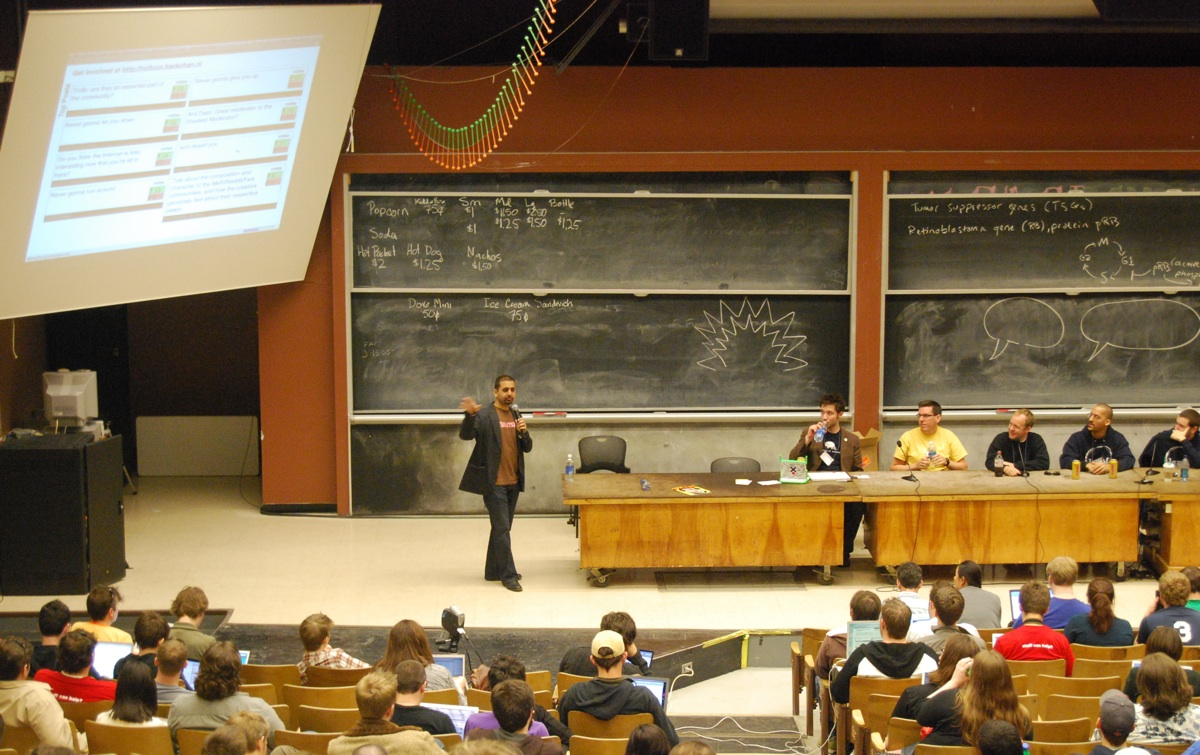
\includegraphics{figures/backchannl/roflcon_photo.jpg}
	\caption{A view of the physical setup for a \emph{backchannl}-enabled event.}
	\label{fig:backchannl_physical}
\end{figure*}

Although the public displays showed only the top eight posts, the web interface maintains a chronological listing of all the posts that had been submitted during the session. As posts receive positive votes, they tend to rise in the ranking and will eventually reach the top eight and are projected on the main screen. The web interface from which votes are cast and items are submitted can be seen in Figure \ref{fig:backchannl_screenshot}.

When a user first loads the site, they are asked to identify themselves with a name and affiliation. This information was included with any posts that a user made. Votes were publicly anonymous, but were tracked internally with the voter's name to prevent multiple-voting. Identity is easily changed and no formal account registration system is included. The implications of how identity is handled in this system are discussed later in the paper. 

\begin{figure*}[t]
	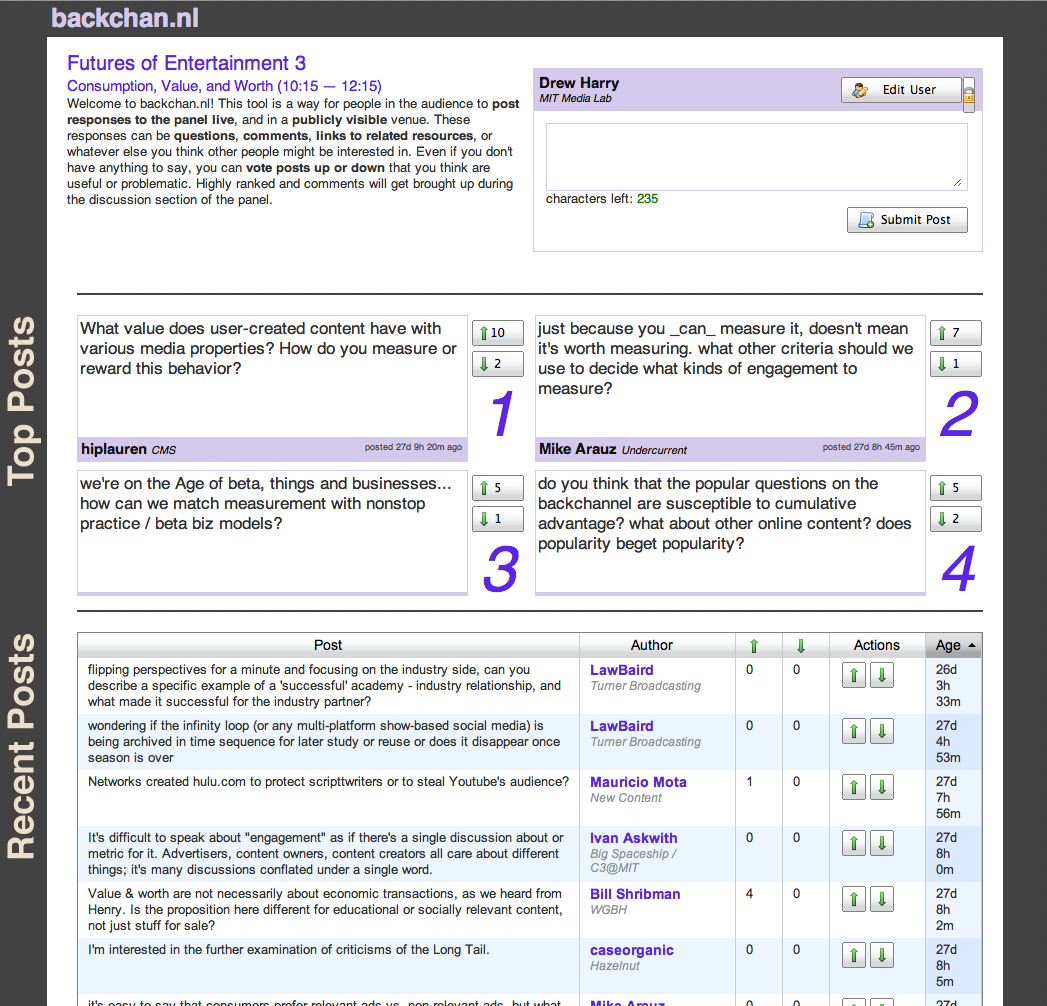
\includegraphics{figures/backchannl/backchannl_screenshot.png}
	\caption{A screenshot of a \emph{backchan.nl} event in action.}
	\label{fig:backchannl_screenshot}
\end{figure*}

\section{Observations}
Although the \emph{backchan.nl} system was designed to be used at one specific event, the success of the tool at that event led to many subsequent inquiries for future deployments. Over the life of the project thus far, \emph{backchan.nl} has been used at hundreds of events. We've had over $13,000$ unique users (though this number is artificially high; see discussions of identity issues in a later section), nearly $19,000$ items posted, nearly $60,000$ votes cast. The events we've tested at have included large events with hundreds of audience members and smaller scale events with audiences of fewer than $100$. Most of these events have been panel discussions of some sort, though we have used it for presentation sessions as well.

For the sake of analysis, we will focus on two of our largest scale deployments that share many characteristics but resulted in significantly different experiences. The first event was the Futures of Entertainment 2 conference. This event was our original deployment target, so its structure informed many of our design decisions. The conference was single track and each session was a two and a half hour panel discussion. Panelists gave brief personal introductions, after which discussion amongst panelists was managed by a moderator. The first two thirds of a session were predominantly guided by pre-prepared questions from the moderator, while during the final third, questions were solicited from the audience. We knew from previous years that the conference audience was likely to have large numbers of laptop users and wireless Internet access in the conference venue was known to be excellent. The audience was largely entertainment industry professionals interested in exploring industry issues from an academic perspective.

The second venue was ROFLcon, a two-day conference exploring Internet culture with panel discussions involving significant figures from the Internet community. The convention had multiple tracks, and \emph{backchan.nl} was only used in the biggest presentation space on the second day of the conference. ROFLcon's attendees tended to be much younger than the Futures of Entertainment 2 audience. The ROFLcon audience included many more students and was generally rowdier and more exuberant. It was not uncommon for audience members to interrupt discussion by shouting something at panelists. Anecdotally, this was many attendees first conference experience. More general descriptions of the atmosphere at ROFLcon can be found in popular media coverage of the event. \citep{Raftery:2008vd}

In terms of their overall format, these two conferences were quite similar; both focused on panel discussions, took place in similarly sized auditorium spaces, and had technically savvy audiences likely to have laptops for accessing the system. Despite this, the audience of each conference used the system in very different ways. In this section, we present and compare usage data between these two conferences.

\subsection{Usage Data--Futures of Entertainment}
Over the course of the five sessions in the conference, there were 125 distinct users. Most names and affiliations were reasonable, with only a handful of completely anonymous names chosen. The use of pseudonyms or nicknames was generally rare. 

These users posted a total of 224 items, with a mean of 37.6 questions per panel and a mean of 20 questions per each morning introductory session. Across all sessions, we observed a rate of question submission of 0.26 posts per minute.

\begin{marginfigure}
	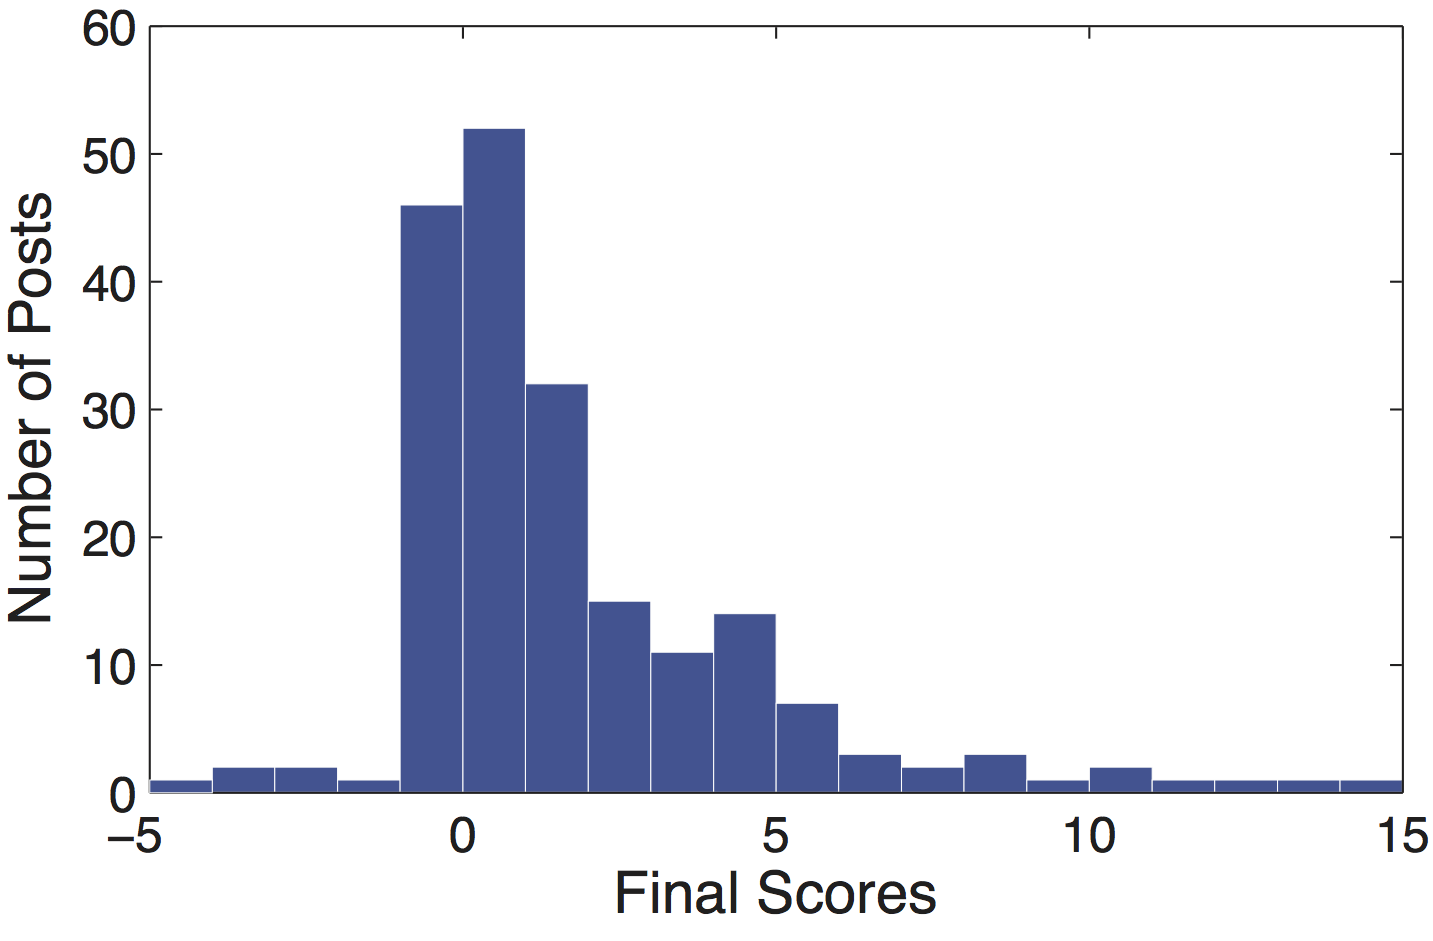
\includegraphics{figures/backchannl/final_scores.png}
	\caption{Histogram of the final scores of posts.}
	\label{fig:final_scores}
\end{marginfigure}

There were a total of 676 votes, with the average post receiving 2 votes. The vast majority of votes were positive: there were 568 positive votes compared to 108 negative votes. The distribution of final scores for posts is shown in Figure \ref{fig:final_scores}. Votes were cast at a rate of 0.78 per minute.



\subsection{Usage Data--ROFLcon}
ROFLcon had five primary sessions that used \emph{backchan.nl}. We observed 450 different usernames, although there are a very large number of pseudonymous names and many duplicate IP addresses recorded. Over the course of those sessions 420 items were posted, at a rate of 1.08 per minute.
There were 1667 distinct votes, recorded at a rate of 4.27 per minute. Of those votes, 1142 were positive, 525 were negative. 



\subsection{Post Contents--Futures of Entertainment}

Over the course of the conference, we observed a number of different categories of posts. Early on in the first panel (and in every subsequent panel), alternative backchannel options set up by audience-members were advertised on the \emph{backchan.nl} system. The first two posts in each panel advertised a Skype public chat and an IRC channel. Private chat was not an inherent feature of our tool, and we were surprised that the first submitted items were advertisements more than questions. In subsequent panels, these postings occurred very quickly, just as the conversation was commencing. Neither channel sustained the same level of involvement as the \emph{backchan.nl} system itself, but its position as a screen visible to all participants in the conference empowered audience-members to create and publicize their own alternative channels. We view the opportunity for the audience to co-opt the channel for competing tools as a demonstration of our commitment to an uncensored channel. Furthermore, such postings highlight the utility of the \emph{backchan.nl} system for audiences to self-organize, and to mediate their own conference experience. These kinds of informational posts didn't score well, and were often the first posts pushed outside of the top eight as soon as questions targeted at the presenters started to be submitted.

During panels, the bulk of popular postings were questions targeted at the panelists. These questions varied in specificity from follow-up questions to panelists (``I would love to hear more about buzz marketing - how it actually works, and how clients want it to integrate it with more traditional methods.") to general synthetic questions (``What's the role of Social Media in advertising and Convergence Culture?").

The other most popular posts represented public sentiment in some way. Near the beginning of the third session, someone posted ``Can we make sure some more questions from the board get answered this time? xthxbai.'' This was the sixth most voted on item in the entire conference. Later in the conference, someone else asked the second most popular question: ``So, is NOW the time the panel should turn some attention to these excellent user-generated questions?'' There was also a complaint about temperature in the auditorium.

Among questions that failed to attract significant attention and votes, there were a number of common themes. Posts that didn't feel sufficiently question-like tended to get passed over. The same was predominantly true for funny and snarky comments. 

\subsection{Post Contents--ROFLcon}
For the most part, items on the backchannel at ROFLcon fall into similar categories as those at Futures of Entertainment. The biggest difference was the balance. There were fewer questions for panelists, but some were certainly generated that were subsequently asked of the panelists, e.g. ``Moot, what is your favorite 4chan meme?'' As at Futures of Entertainment, these items tended to be well received. Most of the top posts in each session were a question for the panelists of some sort.

A significant majority of the posts, however, were not questions. There was a constant flood of jokey posts, for instance: ``WAKE UP SHEEPLE, ALEXIS DID 9/11'', which combines a number of popular Internet memes about a notable community figure (Alexis), a satirical exclamation from the site Alexis runs (``wake up sheeple!'') and 9/11 conspiracies. The success of this kind of post varied widely. Sometimes they were wildly successful, but the vast majority of them languished in obscurity and never made it to the top eight. ROFLcon also had many more announcement type posts like ``::abuses backchannel:: Someone lost a Lumix camera yesterday. Find Susannah on the ROFLTeam to describe it/pics on it.'' As at Futures of Entertainment, messages like these were never highly rated, but did get visibility at the start of sessions. They were rarely submitted later in a particular session. This indicated an understanding that there were phases in a session when different kinds of posts were more or less appropriate. 

ROFLcon's use of the backchannel was much more playful than at Futures of Entertainment 2. This audience was quite familiar with manipulating social tools like this and so pushed the system to its limits. In one session, users engaged in a wide-spread coordinated attempt to rig the item rankings. Eight posts were made containing parts of the lyrics to Rick Astley's ``Never Gonna Give You Up.'' \citep{Anonymous:2007ti} Users then voted these items up and down to make them appear in order in the top eight, attempting to ``rickroll" the audience. ``Rickrolling" — forcing an unsuspecting public to watch/listen to Astley's song — was a relatively popular Internet meme at the time of the conference. The same user name can't vote more than once on an item, so users participating in this process quickly switched between pseudonyms to trick \emph{backchan.nl} into letting them vote again. When they were lyrics were finally in order, someone in the audience yelled ``WE DID IT'' and there was spontaneous applause for their achievement. In this way, users demonstrated a clear internalization of the system dynamics and co-opted the system for their own playful ends. We believe this shows the power of the system; we believe that users only play with systems that provide a meaningful stage. Pictures of his happening are available in \citep{Chillag:2008wr}.

\subsection{Voting and Posting Patterns}

\begin{figure*}[t]
	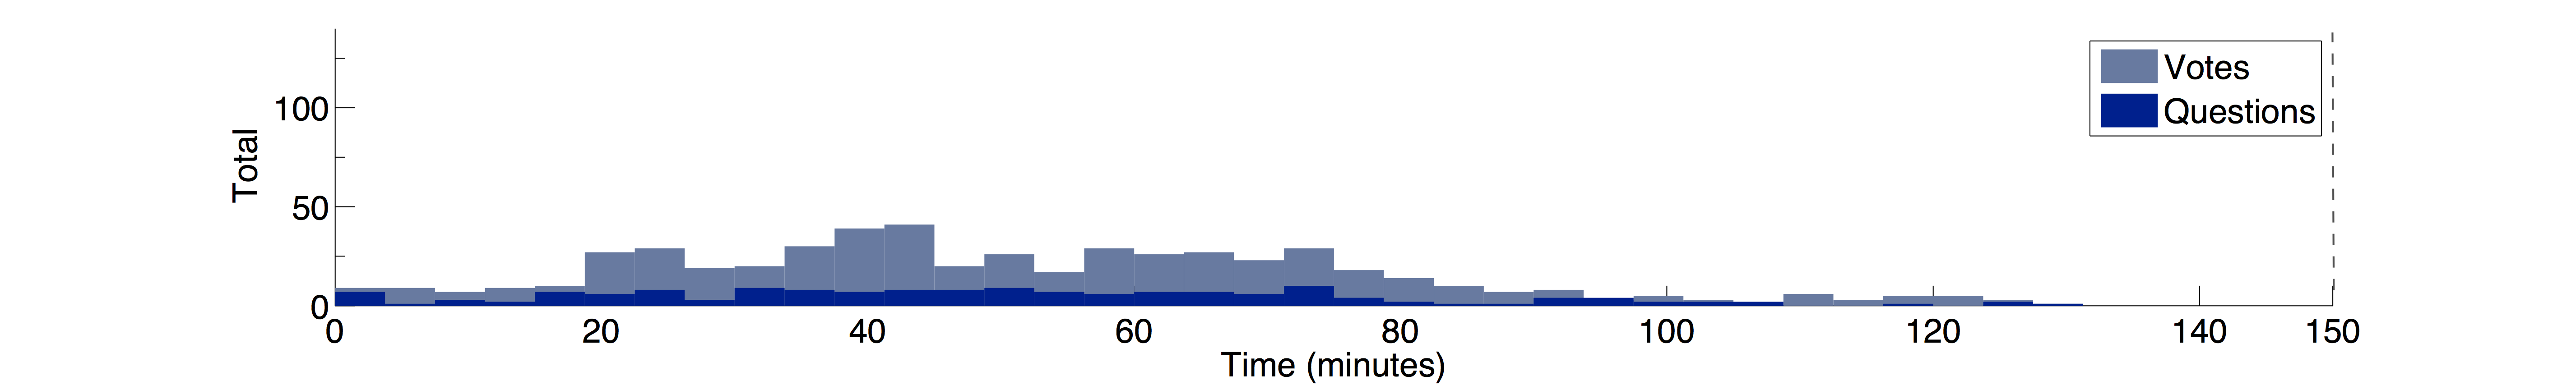
\includegraphics{figures/backchannl/foe2_posting_history.png}
	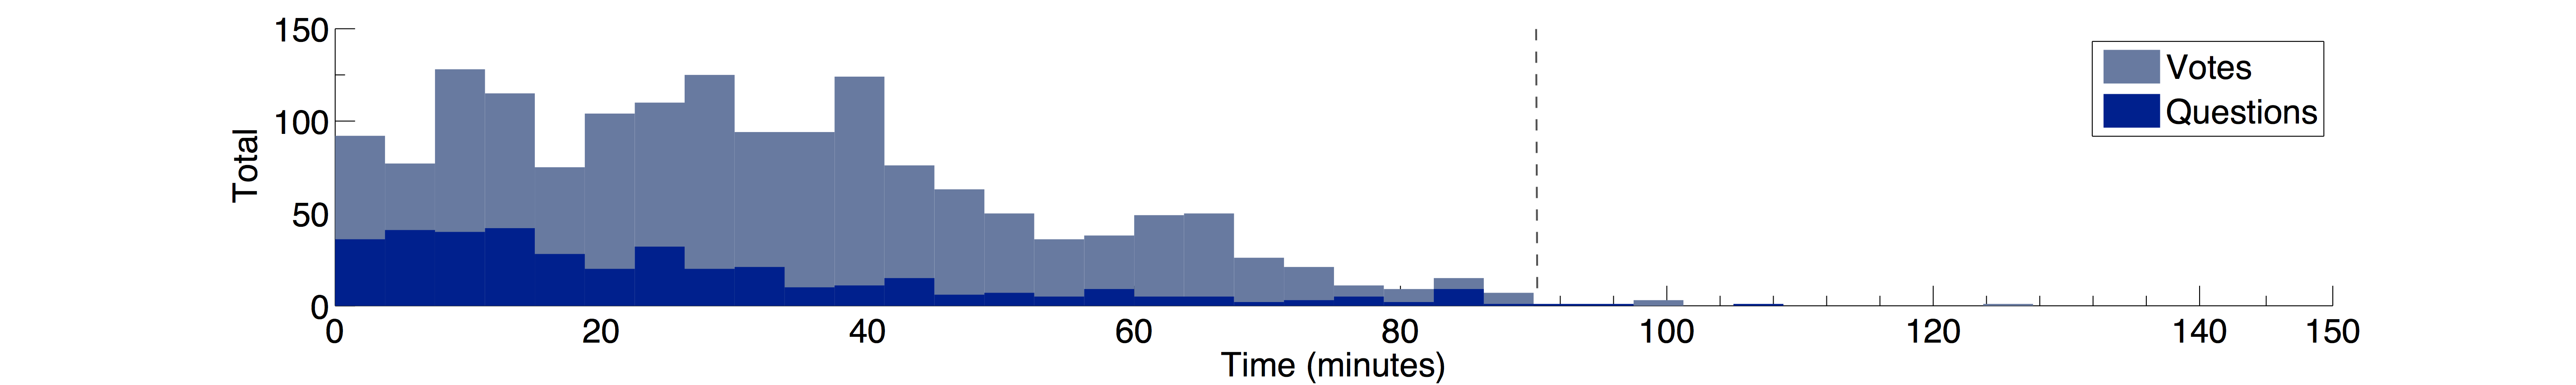
\includegraphics{figures/backchannl/roflcon_figure.png}

	\caption{Accumulated posting and voting events over time. The dashed line marks the duration of sessions in each event. Top: Futures of Entertainment, Bottom: ROFLcon.}
	\label{fig:posting_time_patterns}
\end{figure*}

Over the course of each session, voting and posting patterns emerged that depended quite a bit on the organization of the conference sessions themselves. As seen in Figure \ref{fig:posting_time_patterns}, most of the activity of both posting and voting occurs around the same times. Overall, participation decreases substantially in the second half of every session at Futures of Entertainment 2. This has two possible explanations. Official question time for each panel started between 90 and 120 minutes into each session. Audience members might have chosen to ask questions themselves rather than rely on the backchannel system, given the opportunity. The decline might be a result of users misunderstanding the ranking system and assuming that new posts were unlikely to reach the top eight with so many highly rated posts already submitted. We saw a similar falloff in ROFLcon, though it wasn't as significant. This is closely related to our discussion of tempo later in this paper – it might be the case that this is simply a function of a poor selection of the time constant for these long sessions. 

What is notable about the ROFLcon participation rates is the high number of questions very early on in a session. This is likely because the ROFLcon sessions were personalities the audience was largely already familiar with, and so audience members had questions prepared before the panelists said anything.

\begin{marginfigure}
	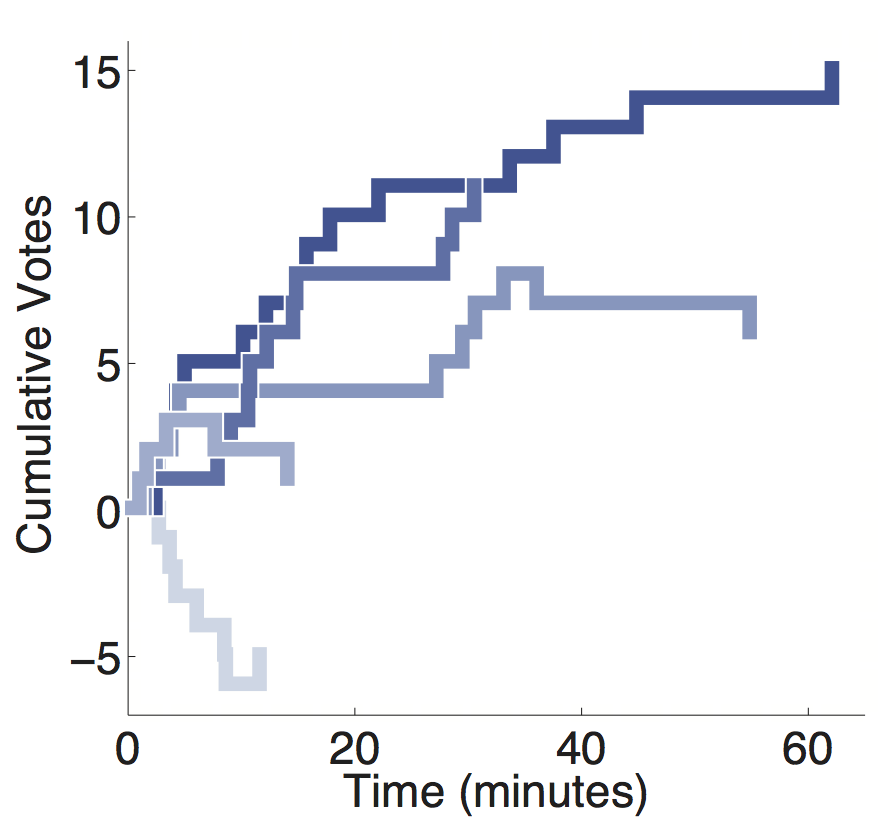
\includegraphics{figures/backchannl/cumulative_vote_histories_colors.png}
	\caption{Tracing the evolution of 5 posts over time. Time 0 is normalized to be the moment the post was submitted. Traces end at the last recorded vote on that item. Notice that the majority of voting on a post happens early in its lifespan.}
	\label{fig:post_score_evolution}
\end{marginfigure}

The voting timelines of a number of different posts are displayed in Figure \ref{fig:post_score_evolution}. In most cases, the voting in the first five minutes of a posts lifetime indicate whether or not it was going to become popular. Posts were rarely contentious—although many posts had some negative votes, they were usually predominantly positive or predominantly negative. These patterns are not unlike those observed in work studying Digg and Reddit, internet-wide systems with a similar voting design. \citep{Lerman:2006wq}


\subsection{Backchannel/Frontchannel Integration}
Over the course of the Futures of Entertainment 2 conference, \emph{backchan.nl} was frequently integrated into the foreground conversation. Although the moderators came to each session with a set of prepared questions, most of them quickly went off the script and integrated the posts from the audience into their questions. Often, the moderator would combine a few different questions into a single broader theme and put that question to the panelists. This process was almost always explicit. The moderator would verbally acknowledge the source of the questions, which ones were being combined, and the audience members who asked the original questions. The audience began to expect this kind of behavior and complained when they felt moderators weren't integrating backchannel questions enough. While this also occurred at ROFLcon, the increased non-question ``noise'' meant that moderators had fewer options to choose from. They almost exclusively ignored the funny posts, which really didn't need to be addressed explicitly.

After the Futures of Entertainment event, it became clear that we needed a way to dismiss posts that had been addressed by the moderator. For subsequent events (including ROFLcon) we had some moderation tools that allowed us both to mark a post as answered (reduce its points to zero but still display it in the upcoming list with a checkmark) and ``remove'' a post (remove all user-visible history of the post). The challenges inherent in moderating a system like this are described later in this paper.

Panelists could also see the backchannel, and would sometimes pull questions from the backchannel into their responses. This worked particularly well because the panels at both events were very discussion oriented and opened-ended.

\section{User Responses}

In general, users and presenters were very positive about the \emph{backchan.nl} experience. At Futures of Entertainment, conference volunteers conducted interviews with participants after the conference finished, and some participants had comments about the backchannel system in particular. One audience member thought ``the ability of people to vote for what they were interested in was great.'' Another participant particularly appreciated that the system ``gave [audience members] opportunities to participate in direct ways.'' Informal chatter at ROFLcon was similar. Moderators tended also to enjoy the system, although they reported having to rethink their moderating approach significantly in light of \emph{backchan.nl}. Over the lifetime of the tool, moderators who have used it more than once are quite positive about its role in panel events, and the organizers of both ROFLcon and Futures of Entertainment requested \emph{backchan.nl} at their next events.

Users and presenters in sessions involving \emph{backchan.nl} expressed a number of common concerns about the system. We collect and address those issues here.


\subsection{Distraction}
In general, users and presenters were very positive about the \emph{backchan.nl} experience. At Futures of Entertainment, conference volunteers conducted interviews with participants after the conference finished, and some participants had comments about the backchannel system in particular. One audience member thought ``the ability of people to vote for what they were interested in was great.'' Another participant particularly appreciated that the system ``gave [audience members] opportunities to participate in direct ways.'' Informal chatter at ROFLcon was similar. Moderators tended also to enjoy the system, although they reported having to rethink their moderating approach significantly in light of \emph{backchan.nl}. Over the lifetime of the tool, moderators who have used it more than once are quite positive about its role in panel events, and the organizers of both ROFLcon and Futures of Entertainment requested \emph{backchan.nl} at their next events. 
Users and presenters in sessions involving \emph{backchan.nl} expressed a number of common concerns about the system. We collect and address those issues here.

\subsection{Presentation Preemption}
Presenters were also concerned that questions would be posted to \emph{backchan.nl} during their presentation that they would answer later in their presentation. Some moderators at Futures of Entertainment 2 expressed concerns that the system placed pressure on them and the panelists to address the audience's concerns first. This concern was also voiced at the handful of non-panel presentations we have run with \emph{backchan.nl}. In these situations, we would typically turn the projection off during the presentation itself and then back on during the question period. During the projection black-out, users could still participate, but the audience as a whole could focus on the presentation materials. Despite presenters' fears, we did not see many instances of the audience pre-empting presentation material with questions.


\subsection{Replies}

Many users lamented the lack of an explicit reply structure in \emph{backchan.nl}. Audience members frequently made explicit comparisons between \emph{backchan.nl} and services like Twitter and IRC, which both have been used in conference situations to provide backchannel conversation. In some deployments these conversations took place over \emph{backchan.nl} itself and became quite contentious. The core complaint in most instances had to do with the lack of a way to distinguish the timing of posts or to indicate that a post was a response to an earlier posting. Some users tried to adopt the ``@username'' format of Twitter, but often these posts would get voted into the top eight without the post it was replying to, decontextualizing the response and confusing audience members who weren't using the tool on a laptop. Over the course of an event, users have almost always moved beyond their initial attempts to use \emph{backchan.nl} in ways it wasn't designed for and settle into a pattern of posting items that aren't explicitly intended to generate responses from the audience. 

In future versions, we would be interested in better affording responses. From a design perspective, we find integrating replies a challenging and interesting problem. Given our limited projection screen space and the contextual nature of discussions, we're hesitant to display elaborate conversations on the screen. Although filtering moderation systems like Slashdot's have been shown to be appreciated by users \citep{Ratto:2003vs}, we have a non-interactive, low density group display and would have to make a global decision for all users about what threshold is appropriate.

We also don't want presenters to feel (accurately or not) that the \emph{backchan.nl} is home to significant conversations that they don't have any visibility into. This is at odds with our desire to have an uncluttered main projection screen. A successful design will have to accommodate both users' desires and presenters' concerns.

\section{Analysis}

What sets this approach apart from other backchannels is the presence of the backchannel in the physical space. This approach had a few categories of effects, relative to work on non-physically situated backchannels.

\subsection{Content}
The content in this backchannel is markedly different from the content observed in chat-based backchannel implementations \citep{Yardi:2006uk,Cogdill:2001fp,Golub:2005ws,Rekimoto:1998jy}. While the vast majority of posts in this system could be classified as ``Work" messages in McCarthy's categories, they were usually focused on a specific audience — the panelists. While panelists have sometimes been involved in backchannels in other systems, participants in a backchannel have never known that all panelists could easily see their comments. Importing the backchannel into the conference space itself makes it clear who is seeing what's posted. This increases the stakes of backchannel communication, as it enjoys an audience that extends to those not actively using the interface itself.

This played out in different ways in the two conferences. For Futures of Entertainment 2, the increased stakes meant users mostly took the system seriously and there were few snarky or critical comments. This is no doubt influenced by the fact many in the audience were attending for professional purposes, either as representatives of their businesses, for networking, or to learn more about their industry. The more playful approach of the ROFLcon audience reflects that community's interests and normal mode of interaction. Higher stakes made users likely to use the system, but content was similar to what they might have normally posted in an online-only discussion. In this way the implementations were not so different; both offered a material representations of the different values of the communities present. This echoes the behavior of the children in \citep{Chesnais:uh} who, even in the face of adult disapproval and public attribution of their messages continued to submit messages that the organizers found objectionable. 

\subsection{Adoption}

Backchannel adoption is often a serious problem. \citep{Orlikowski:1992tza} Having a physical representation of the backchannel in the space serves as a constant reminder about how to get involved in the backchannel and what is currently happening on it. This provides an effective hook to get new users involved. In particular, the appearance of posts that an audience member thinks is great (or terrible) and the promise that they can help promote or demote it is a powerful incentive. 

The moderators played a key role in \emph{backchan.nl} adoption. After a moderator effectively demonstrates how \emph{backchan.nl} can be used, users quickly build an expectation about its use in future sessions. As with the adoption of other social technologies, it was important for the audience to see that the tool was being taken seriously and that their interactions across it were meaningful to the conference organizers.\citep{Orlikowski:1992tza} This was most clear when the audience co-opted the system to complain about the lack of attention the board was receiving. Indeed, the moderators explicitly responded to each major complaint that appeared on the projection during Futures of Entertainment 2. The chaotic nature of the items at ROFLcon sometimes precluded acknowledgement, though issues with sound were frequently addressed in response to audience comments. 

The physical arrangement in the room further underscores this organizational support. Although people in the audience were able to set up their own backchannels using other software, having a projector and a screen in the room demonstrated the material commitment of the conference organizers to this tool. Although it's possible to imagine situations in which \emph{backchan.nl} might be marginalized by user-organized backchannels, this didn't happen in any of our deployments and we suspect a large part of that is the physical-ness of the design. It's hard to simply ignore a display in the presentation space in favor of a virtual-only conversation space.



\section{Backchannel Configuration}
Based on our experiences deploying the \emph{backchan.nl} system, it has become clear to us that there are a number of ways in which a backchannel can be configured that would make this tool both more broadly applicable and more finely tuned for the needs of specific groups of users. In this section, we discuss two major design questions: how should post scores change over time and how should users' identities be represented in the backchannel? In both cases, we argue that a mediated social space like \emph{backchan.nl} would substantially benefit from having configuration options that adapt it to different situations. In much the same way that you might arrange the chairs in a room differently for a lecture versus a group discussion, so too should mediated social spaces have a range of options that foster different social situations.

\subsection{Tempo and Time}

There are a number of modern systems that provide some sort of ``top" list of items. \emph{Digg} and \emph{Reddit} are perhaps two of the most notable (and straightforward) examples of this service; users submit URLs, which can be voted on by other users and by some metric the items are sorted and top items are displayed prominently. These systems (like our system) face an interesting algorithmic challenge: how do you keep the top items changing fluidly such that popular items rise to the top but previously popular items don't linger too long? Certainly, a rank ordering of items by the number of votes is not generally going to be sustainable; older items will tend to accumulate the most votes and make it hard for newly posted items to graduate to the ``top" list of items. In designing a technique for ranking posts, we had a number of goals in mind:

\begin{enumerate}
\item{Highly positively voted posts should get a high ranking.}
\item{New posts should eventually displace older posts.}
\item{Contentious posts should be rewarded somewhat, but less than uniformly well received posts.}
\item{Posts that continue to receive attention over time should stay highly ranked.}
\end{enumerate}

The score is comprised of two factors: an age factor and a vote factor. The vote factor (where $U_p$ and $D_p$ are the up and down votes of a given post p, and where $\overline{(U+D)}$ is the average umber of total votes across all items in the session) is:

\begin{equation}
voteFactor(p) = \frac{kU_p}{U_p + D_p} + \frac{U_p + D_p}{\overline{(U+D)}}
\end{equation}

The first term rewards posts with many positive votes, while the second term promotes items that have a high vote total relative to all posts in the system. In general, the first term rewards positive votes while the second term rewards negative votes. The balance between those terms is set by the constant $k$. 

The age factor (where $t_{p,v}$ is the timestamp of a specific vote on item $p$ and $t_{now}$ is the current timestamp) is:

\begin{equation}
ageFactor(t_p, t_{now}) = \frac{\overline{(t_{now} - t_{p,v})}}{\tau}
\end{equation}

The average time difference was computed for the most recent (up to) five votes on each item. The time constant $\tau$ varied in our experiments, but something on the order of $10^4$ was usually effective.

The two factors are multiplied together to generate the final score.
The main difference between our ranking system and those discussed in \citep{Anonymous:8tu} is that ours measures time not on the basis of the initial posting of an item, but on a moving average of the ages of its votes. In this way, an old item that receives new attention from voters is rewarded.

One of the downsides to this approach is that the points used for internal rankings are not typically made visible to users. This leads to many situations in which an item with few votes is more highly ranked than an older item with many more votes. Although this seems dissonant, users have very rarely commented on it when using the system. Perhaps popular adoption of similar systems has made familiar the notion that voting helps promote something, but that rankings are not strictly tied to votes.

The time constant in the system plays an important role in configuring the space. The time constant sets a sort of tempo for the system; if items decay slowly the top ten is a sort of low-pass filter, showing items that have been of enduring interest to the audience over a long period of a time. This might be useful in a session where the \emph{backchan.nl}'s role is to accumulate questions when there are only a handful of panelists and each panelist speaks for quite a while before there are questions. Conversely, if items decay quickly, the top listing will turn over quickly, exposing a very high-pass view of the audience's interests. This might work well with a panel where the topic is shifting quickly or there are many panelists speaking for a short time. Which kind of time constant is appropriate also has to do with the number of participants. If there are more voters, faster decay makes more sense because more votes will offset the time decay pressure of the ranking equation.

Returning to the goals for a ranking system that we proposed, it is important to note that these goals are specific to the conference situations we were initially designing for. In line with our longer-term interest in describing the ways that a backchannel can be configured for different situations, it is easy to imagine conference situations when our goals don't necessarily make sense and we might design a different scoring system. For instance, in a paper-oriented conference like CHI, our goal of having a ``live" list of questions receiving attention might not be appropriate. Instead, a naive ranking mode in which questions accumulate during someone's talk and are ranked purely by their positive and negative votes would be a useful way of identifying the best questions for the end of the talk. This is biased against questions that might be raised towards the end of the talk, but that might actually be a benefit. The backchannel could act as a counterpoint to the existing structure in which questions often focus on the end of the talk because it's freshest in the audience's mind.


\subsection{Identity}
As in all mediated social systems, how identity is represented in the system can have profound impacts on the behavior in that system. In our design, identity is handled in a very informal way. Users can enter a name and affiliation, but it is trivially easy to change your personal information. This keeps the threshold for involvement quite low, and we built the system this way to encourage more use. In general, the tradeoff in building identity systems is between low thresholds that encourage use (like our model) and systems that have higher costs to join, but also provide more reliable signals about identity between users. An extreme example of a higher cost identity system might require credentials from a trusted source, but such a system would keep out people who didn't have such credentials or didn't want to expose that much information about themselves. Given our initial venue, we built a system that was biased towards a lightweight identity.

We found (as discussed earlier) that in our first deployment at the Futures of Entertainment 2 conference, there was very little identity play, and our decision promoted productive discussion. This is in stark contrast to ROFLcon, where playful and funny posts outnumbered traditional questions. This playful attitude towards identity is evident in the usage data. There were a much larger number of unique users at ROFLcon of which the vast majority were pseudonymous.

From a design perspective this comparison makes clear that different identity structures make sense for different audiences and presentation structures. When considering the design of future backchannel systems, we believe a range of identity options should be offered. Beyond the extremes of no registration and trusted certificates, the system could require email verification or track IP addresses, which would increase the costs to changing identity. In this middle ground, identity in the system is still easily gained, but changing identities is more problematic.

Archiving also plays a role in identity. By changing what kinds of behavior are stored in the system, low-cost identity forms can accrue more costs to changing. If users see other users with rich histories in the system, they will tend to be rewarded for their history by other committed users. \citep{Resnick:2002hf} In this context, users with a history of submitting useful questions can easily be distinguished from someone with a throwaway account. The costs of this kind of pseudonymity have also been explored from a theoretical perspective by\citep{Friedman:2001ti}. Indeed, what about users' behavior is archived and made publicly available is another important axis along which a backchannel might be configured.

\subsection{Democracy and Moderation}
This system encodes a basic democratic principle: the best items will rise to the top based on the aggregate will of the audience. There are limits to this principle, though. As mentioned earlier we quickly discovered that we needed some sort of moderation vocabulary. We settled on two basic actions: ``answered'' which sets an item's points to zero and ``remove'' which removes all visible record of the item. Because moderators who used early versions of this system had requested this feature, we hoped that they would also take responsibility for making the decision to demote or remove a post. In practice, this was too much of a burden on them, especially in situations (like ROFLcon) where participants were regularly submitting offensive items, and moderation didn't just involve marking ``answered'' items. 

In practice, one of the authors would sit in the audience and take responsibility for moderating posts. We moderated with a very light hand, marking as answered only those posts that were explicitly mentioned by the moderator and that panelists seemed to answer and removing only those posts that were broadly offensive. Of course, there are substantial grey areas in these criteria. Questions were sometimes posed to panelists and subsequently evaded. Presumably the author of that question would like to see it remain in the top eight, even though the panelist ostensibly responded to it. ROFLcon offered other kinds of posts that we struggled to respond to. In the process of arranging song lyrics in the top eight slots, all other submissions were pushed out. After the ordering was successfully achieved and publicly acknowledged, should we remove them? Indeed, humorous posts in general tended to clog up the top eight because they couldn't really be ``answered'' and so there was no clear contract between the moderator and the audience about how they should be handled. Furthermore, the sheer achievement resonated with the spirit of the conference itself. In the case of the song lyrics, we left them on the board hoping that the audience would subsequently down-vote them to clear the board for new content. This turned out not to be the case, and \emph{backchan.nl} was largely useless for the rest of that panel.

These tensions between keeping the tool effective and letting some version of a democratic process run its course pervade social tools like this. In this case, our approach was to at the very least maintain an open approach to moderation. Posts that were demoted were clearly noted with icons, and all their original votes were still shown on the website view. In this way, the moderator is at least accountable for her actions. In the same way that the audience spoke out against panel moderators that were clearly ignoring \emph{backchan.nl} questions, they could co-opt the tool to protest moderation decisions they disagreed with.

As discussed with respect to tempo and identity, we argue that configuration has an important role to play here. Because the standards and desires of different communities can vary widely, it makes sense in some situations to devolve the moderation controls to the users. Digg, for instance, has systems that allow users to ``bury'' a post they think is inappropriate for some reason. Of course, the risk of tools like this is that they can be easily abused by organized groups of users that want to suppress certain points of view. An effective compromise is ``flagging'' systems used notably by \emph{Craigslist} and \emph{Metafilter}. In this model, users could flag items as being ``offensive'' or ``answered.'' Moderators can use these flags as a proxy for the audience's attitude about specific posts. Having a person making an interpretive decision from this data makes it much harder for groups of users to manipulate an automatic moderation system. There are roles for both of these moderation strategies, as well as the simple benevolent-moderator model we used during our testing. This is the final axis that we propose should be available for configuring backchannels. 


\section{Conclusions and Future Work}
In this paper, we have demonstrated how integrating a backchannel into the physical space of a conference can create effective new ways for the audience to interact with panelists, moderators, and other audience members. While this approach doesn't necessarily work with chat-based backchannels, our posting approach was both a legible interaction metaphor and made the backchannel more appropriate for public projection.

There are a number of incremental changes that could be made to improve this system. While the system is currently adapted to posting snippets of text, it could easily be diversified to include many more types of objects. Links to web resources, polls, and discussion threads could all be promoted to first-class objects in the system. An embedded chat interface would also be helpful, providing live discussion opportunities. We are also interested in including some sort of reply mechanism for web-users that does not adversely impact the projected non-participant view. 

More broadly, we're interested in the ways that mediated interaction spaces can be configured for supporting different kinds of social situations. We discuss the ways that tempo and identity function in this particular system as a way of laying out a broader structure for the relationship between these kinds of design decisions and the kinds of interactions they create. 

Finally, we're interested in the potential of backchannel systems like this one as a way to involve remote participants with co-located participants. Remote participants are often marginalized and forced to rely on a local advocate to interrupt the flow of conversation and check for questions from remote users. Our backchannel approach offers a way to more fluidly involve remote participants by encouraging both local and remote users to interact through the same mediated system. This blurs the lines between local and remote participants and could counteract some of the disadvantages of being a remote participant. Although for the most part the deployments we discuss did not have significant numbers of virtual participants, our future work in this area will explore the implications of this system on remote participants.

\chapter{Tin Can}
\label{ch:tincan}

In the introduction, I argued that taking a ``beyond being there'' approach to designing collaborative interactions can yield powerful results. I have shown in the past two chapters how designs that aim not to create the experience of ``being there'' but instead to imagine new kinds of relationships and interactions can be both meaningful to users and improve on traditional ``being there'' approaches to mediated interaction. In this chapter, I will introduce \emph{Tin Can}, a tablet-based application to collaborativly track discussion topics and ideas in a seminar-style discussion classroom. Based on our study of this system, I will argue that we have created a system that remains quite useful even when everyone using the system is face-to-face and could eschew the system entirely if it wasn't useful to them. Looking forward,  \citet{Hollan:1992tz} argue in 1992 that ``no one seems to be asking the question, ``what would happen if we were to develop communication tools with a higher information richness than face-to-face?'''' I view \emph{Tin Can} as one of many potential answers to this question.

In a classroom using \emph{Tin Can}, each student uses his or her own tablet to share text ideas in a synchronized, visual environment. The system is designed to promote diverse participation and increase engagement. Using this platform, we observed twelve class sessions and conducted interviews with the participating students. Instead of simply introducing an additional text-based communication channel into the classroom, we find that the system creates a new ``stage'' (in the Goffman sense) on which students could perform in ways that the main spoken stage could not support. This stage coexists with spoken communication, and augments how students attend to the material and each other. We conclude that spoken participation alone poses barriers for some participants and the addition of a non-oral, text-based stage can help establish more equitable, diverse, and engaging discussions in the class.

% the other options for this are "Computer-supported cooperative work" or "Collaborative computing". Bit of a wash which one we do.

\section{Introduction}

The physically co-located small group discussion is often viewed as the gold standard for effective collaboration and communication.  It can provide a space for participants to voice their opinions and can readily lead to deliberation and collective problem solving \citep{Burkhalter:2002vg}. Not surprisingly, it is often the case that designers seek to virtually reproduce the characteristics and norms of the small group discussion in technologically mediated communication media. \citet{Hollan:1992tz} provide a valuable counterpoint to this approach arguing against viewing experiences mediated by the ``physically proximate'' reality as necessarily superior to those mediated by technology. We have adopted the following challenge: instead of assuming that the small group discussion is good enough and the only appropriate design consideration is its preservation and replication, we seek to appropriately apply the unique properties of a technological system to the established affordances of a small group discussion. We would not deny that face-to-face interaction offers many substantial benefits when compared to interactions mediated by, for instance, a video conferencing system; nevertheless, we argue that there is room to improve the physically proximate small group discussion by intervening in the assumed normal frameworks of turn-taking and attention. \sidenote{Much of the contents of this chapter are drawn from \citep{Harry:2012df}, which represents collaboration between the author of this dissertation and Eric Gordon.}

In this paper, we describe the design and enacted use of a tablet-based system for a discussion-based graduate seminar. Although this is not a common educational venue for intervention (lecture classes are a more traditional venue, e.g. \citep{Kam:2005wb} or \citep{Bergstrom:wl}), it is one in which we identified a number of potential problems with pure face-to-face discussions that a tablet-based system might effectively address. We had two major goals for this work: first, create a class discussion context that encouraged more diverse participation in class; and second, to help students feel engaged and connected to the learning environment. 

To meet these goals, we sought to expand notions of legitimate participation beyond speaking, using the affordances of a text-based communication system. Our system creates an alternate communication space within the learning environment. Typically, in group communication contexts, spoken participation is viewed as the primary or dominant interaction medium, one that is often the target of modification as in, for example, \emph{Second Messenger}\citep{DiMicco:2007ie} or \emph{Meeting Mediator}\citep{Kim:2008ip}. Like the \emph{Cognoter}\citep{Tatar:1991jq} system, our system placed emphasis on the combinatory possibilities of text-based and oral participation in a co-located group communication environment.  Unlike \emph{Cognoter}, however, we focus on enhancing the performative space of group interaction. Consequently, our goal was not to create alternative communication channels; instead, it was to expand the space of performance. As part of this conceptual shift, we argue for moving from the metaphor of a ``front'', spoken channel and a ``back'' channel to the metaphor of a ``main'' performance stage and ``side'' performance stage.

This study seeks to understand how having simultaneously accessible stages in the context of a group discussion affects the methods and outcomes of participant engagement. We start by describing how our system, called \emph{Tin Can}, is related to existing systems that similarly augment face-to-face communication. We introduce the idea of \emph{stages} and contrast it to previous models of \emph{channels}. We then describe in detail the critical design elements of the \emph{Tin Can} application and the class context in which it was implemented. Then, we present the results of the study, based on class observations, process traces, and interviews.  In our discussion, we return to the concept of stages and describe how this formulation of participation can be productive for thinking through how people can interact with additional stages introduced into the dominant context of face-to-face communication. Finally, we discuss some specific insights about the tablet as a platform and describe the extent to which the design met our initial goals and how our results compare to those from past findings in the literature.


\section{Related Work}


% REVISION Unnecessary, I think.
% We situate our work amongst three related categories of systems: systems that augment face-to-face discussions, systems designed for classroom engagement, and systems to support backchannel conversations. We will relate this work to ours both in terms of design as well as (when appropriate) experimental findings.

% we'll include nunamaker etc in that category
% From Chapanis: "A final point of interest is that a subject is much more likely to take control of a voice channel than of a channel or any combination of channels lacking voice." (41-42).  

There is a rich field of research on the topic of augmenting co-present group communication with socio-technical systems.  One significant area of investigation concerns how systems can ``level the playing field'' of face-to-face communication through reflecting information about a group's behavior back on itself. \citet{Karahalios:hu} refer to this as a ``social mirror''; a real-time visualization of social dynamics that is shared by the whole group and can cause changes in group dynamics. They suggest that ``social mirrors become another channel for interaction (or a back channel) and, in the process, become a signal that influences interaction.'' Their exemplar social mirrors measure behavior in an audio channel and visualize different aspects of it on on shared Displays.\sidenote{There are a series of projects in this stream, including table-top interfaces for visualizing machine-recognized topics \citep{Bergstrom:2009fe}, reaching consensus through discreet voting \citep{Bergstrom:2009ej}, or balancing relative participation in group conversations \citep{Bergstrom:2007je}.} This strategy is shared by \emph{Second Messenger}\citep{DiMicco:2007ie} and \emph{Meeting Mediator}\citep{Kim:2008ip}.  In these systems, presenting real-time participation visualizations tended to close the gap between over-participating group members and under-participating members, although in most cases this effect was primarily from over-participating members decreasing their participation. This work demonstrates how visualizing main stage spoken participation in different ways can impact relative participation rates by encouraging individuals to censor or otherwise alter the nature of their communication to correspond with perceived group norms and group behavior.

Another strain of this work is less interested in altering the oral channel of group communication, and more focused on creating separate, productive  backchannels. There are a variety of contexts where people have added communication channels. \citet{Yardi:2006uk} describes how a chat-based backchannel operates over a semester in a class, \citet{mccarthy_digital_2004} describe a similar approach at a conference. This early work focuses on characterizing the kinds of use that occur in backchannels using existing systems like chat, but do not engage specifically with design issues in backchannels. \citet{Harry:2009jh} propose a new design for projecting question-oriented backchannels in panel presentations.  \citet{Yankelovich:2005bx} discuss oral backchannels during remote, audio-conference-based meetings, and the ``social translucence'' research stream (\emph{Rendezvous} \citep{kellogg_leveraging_2006} is most closely related to this work) explores the design of systems to represent engagement in different kinds of mediated social situations.

\emph{Tin Can} is designed specifically for use in a class, and is thus influenced by the systems designed for this specific context. Like much of the backchannel work described above these systems are typically concerned with creating new channels for communication in, for example, a large lecture hall. Bergstrom's lecture class system \citep{Bergstrom:wl} supports question-asking and commenting and the \emph{Livenotes} project \citep{Kam:2005wb} supports taking shared notes on lecture presentation slides. The \emph{ActiveClass} project \citep{Ratto:2003vs} creates a channel between students and instructors for asking anonymous questions during a lecture from PDAs.  Each of these systems seeks to increase participation in very large group settings by establishing separate channels for participation.  Work in this space is typically not focused on directly influencing spoken participation because the expectation is that there is none; the lecturer is (except for question-asking) the only legitimate participant.

% not going to mention Classroom2k because it's about archiving and we're not talking about that now.
\emph{Classroom 2000} \citep{Abowd:1998wp} created a ubiquitous computing environment to create rich records of a lecture. \emph{Tin Can} shares \emph{Classroom 2000}'s interest in generating a record of the class, but takes a decidedly low-sophistication approach to it, relying on members of the class to generate the appropriate metadata instead of a broad technical infrastructure. Although questions play a role in our system as well, they are in-the-moment guides to discussion and not primarily aimed at the professor (indeed, the professor asked many of the questions in the system). \emph{Classroom 2000} is focused primarily on lecture situations, which have very different interaction dynamics than the discussions \emph{Tin Can} supports. \emph{Classroom 2000} focused on adding value (in our terminology) to the main stage performances of the professor, and are not trying to create credible side stages for student interaction.

In \emph{Tin Can}, we take a different approach. We seek to expand the stage of participation by diversifying the sites of performance. In other words, we are not interested in creating better oral or better text-based channels; instead, through their correspondence, we seek to create a rich environment for participation composed of multiple, simultaneous stages.   Perhaps the earliest research to explore this sort of approach is \citeapos{Tatar:1991jq} work on \emph{Cognoter}. They pointed to some interesting problems with creating stages, namely the limits of the ``parcel-post'' model of communication---where a message is sent and subsequently received and interpreted. Although this model works well for written correspondence, they found that within \emph{Cognoter}, because the written contributions were designed to be interspersed with verbal dialogue, it was difficult for users to understand them ``within the time frame of the actual communication'' unless the oral conversation paused while written contributions were processed. In other words, in actual practice, users resorted to channel switching in order to accommodate the written or the oral modes. Another example is the \emph{Thoughtswap} \citep{DickeyKurdziolek:2010wt} project which takes a much more structured approach by interspersing periods of engagement with the system with freeform discussion. In \emph{Tin Can}, we employed a similar model of written communication to \emph{Cognoter} and \emph{Thoughtswap}, but we found that we were able to successfully create simultaneous stages for participation instead of stages one at a time. We will discuss the reasons for this disparity at more length in the conclusions. Work in this space on how alternate communication channels are selected and used owes a clear debt to \citeapos{Ochsman:1974vu} early work on mediated collaboration.

%These systems are focused on adding back or side stages to existing main stages. In contrast, Nunamaker's work on brainstorming and decision-making \cite{nunamaker_electronic_1991} seeks to create a new main stage for the group that strongly structures verbal interaction.



% The early work in this area was most concerned with supporting existing tools or methods for achieving backchannels in various social situations, particularly presentations,  lectures, and meetings. Yardi describes how a chat-based backchannel operates over a semester in a classroom \cite{Yardi:2006uk}, McCarthy et al. describe a similar approach at a conference \cite{mccarthy_digital_2004}. This early work focuses on characterizing the kinds of use that occur in backchannels using existing systems like chat, but do not engage specifically with design issues in backchannels.  

% We are in many ways inspired by the work of DiMicco et al. on \emph{Second Messenger} \cite{DiMicco:2007ie}. The notion of

% I want to work this in somewhere, but since the shift away from focusing on systems it makes less sense here. 
% \emph{Tin Can} also supports significantly more participants than any of these systems, which has major impacts on the kinds of dynamics at work.

% This is a design-oriented way of contrasting the work. Going to try to spend less time on that in this rewrite.
% \emph{Tin Can} shares some of these visualization strategies and is supported by their findings that discussants can feasibly attend to and respond to representations of their interactions while maintaining a conversation. It differs, though, in the level of activity it expects from its users. \emph{Tin Can} offers a distinct communication framework and active curation in contrast to the machine learning techniques frequently employed in these kinds of systems. \emph{Tin Can} also supports significantly more participants than any of these systems, which has major impacts on the kinds of dynamics at work.


% saving these references in case we need them, but we don't reallly need to go that cite-crazy here. better to spend or space on other stuff.
% as described by Karahalios \cite{Bergstrom:hu} 

% REVISION This should be slimmed down in a revision of the related work section, since we're taking the focus off creating an archive. Also, it should focus more on more closely related stuff like livenotes, Bergstrom's backchan.nl like system, and cognoter. 








% 

%  

% REVISION This is a bit wordy. I might try to trim this pretty substantially and just defer the whole conversation to when we actually dig in on the difference. In any event, I think this is either a decent way to introduce the discussion here, or we can salvage it when we do the full discussion later.






% All of these projects share \emph{Tin Can}'s interest in creating new spaces for group communication, and some of these kinds of systems are integrated into the physical spaces the group inhabits. Backchannels are not just focused on co-located groups, however, and Kellogg \cite{kellogg_leveraging_2006} (among others, like \cite{Yankelovich:2005bx}) has addressed how text and audio backchannels can operate in distributed contexts. Most of this work focuses on backchannels as a generalized communication channel, but some researchers, like Nunamaker, focus instead on building formalized systems for brainstorming and decision-making to which (like \emph{Tin Can}) each user has dedicated personal access, but (unlike \emph{Tin Can}) attempt to use the mediated backchannel to structure and drive the front channel interactions \cite{nunamaker_electronic_1991}.


\section {Setting the Stage}

The research questions and goals for the students' experience using \emph{Tin Can} are captured in the main stage / side stage model. We wanted to create a side stage experience where participation was viewed as a legitimate part of class discourse and had a clear impact on the oral discussion. This is in some ways a radical strategy: why should we add technology to a classroom discussion if we want people to be more involved and attentive?


% COMMENT The paragraph that follows is really great. I love that way of framing the problem. (Drew)

\begin{figure*}[t]
\centering
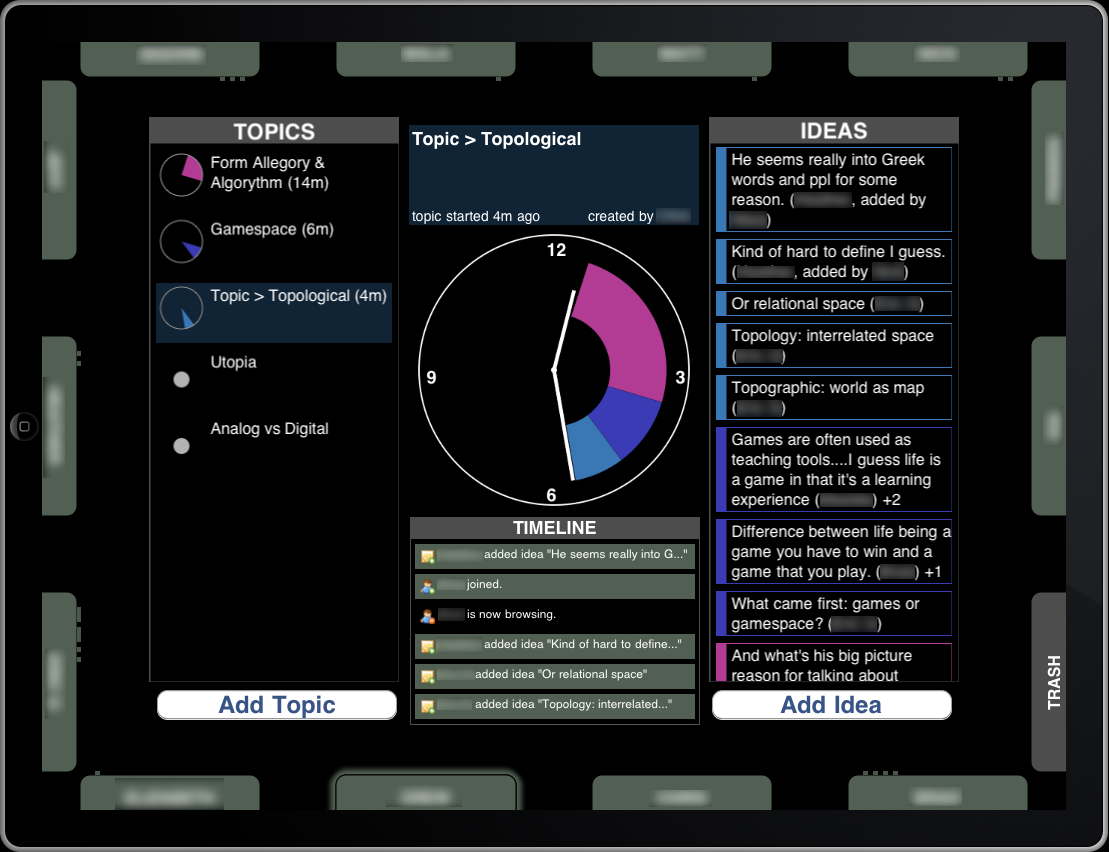
\includegraphics{figures/tincan/tincan_interface.png}
\caption{A screenshot of the \emph{Tin Can} interface running on a tablet.}
\label{f:interface}
\end{figure*}

\begin{figure*}[t]
\centering
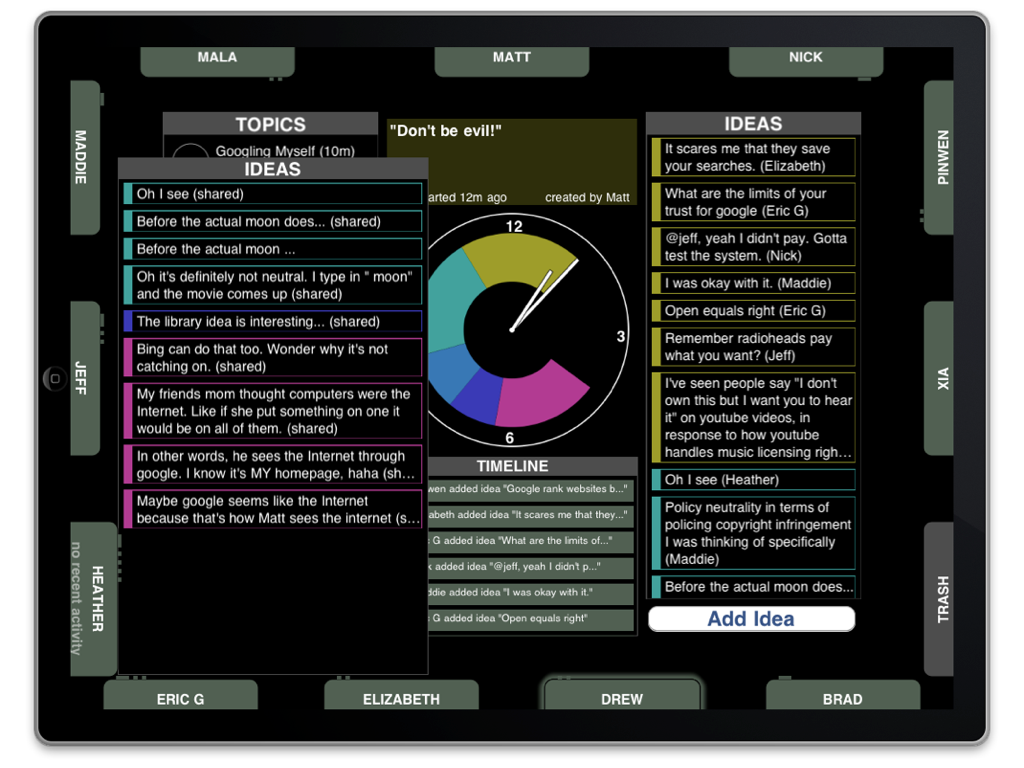
\includegraphics{figures/tincan/tincan-screenshot-with-drawer.png}
\caption{A screenshot of the \emph{Tin Can} interface, with one of the personal idea drawers exposed.}
\label{f:interface-drawer}
\end{figure*}

Traditionally, educators have accepted the quality and sufficiency of the main stage in small groups and eschewed the addition of other communication channels because they might be distracting. A seminar class already adheres to the gold standard of face-to-face communication. It is often assumed that the pressures of the performance are exactly what we want them to be---students talk and the professor evaluates. But there are two faulty assumptions here.  The first is that engagement in a co-present discussion can be manifested only in established methods of performance, for example, speech. And the second is that all students are equally capable of convincing performances. Social psychology research suggests that introverts rely more heavily on written communication to express themselves \citep{Ross:2009gp, Wilson:2010ib}. But when there is only one legitimate kind of performance in a class, when there is only one way to perform on the front stage, the structure of the learning environment may not be as equitable as it could be, and it may not even be as productive as possible, even for extroverts. 

Consequently, when designing for the seminar, we sought to intervene in the established norms of the front stage by adding a well-crafted additional stage. The goal was to create a context for the legitimate performance of the back stage without having to \emph{go away} from the front stage.  As such, we move away from the front/back distinction, preferring the notion of a main stage with a side stage. We sought to design a system where performers could be on both stages at once, where performances were simultaneous, not alternating. Furthermore, the front and back stage as Goffman uses it implies different audiences for front and back performances. Moving to main and side stages reinforces the shared audience of the two stages, which has a big influence on how people perform on each stage and makes it easier to integrate those performances in a meaningful way. We use the terms main stage (face-to-face, spoken conversation) and side stage (text input) to explain the context of performance created as a result of using \emph{Tin Can}.  

% REVISION Try to bring in that quote from the cognoter paper? "Our construction of this distinction is that whiteboard items hold a dual status as elements in the conversation and elements that may be conversed about"
% This quote captures part of the distinction we're going for here. Whiteboards, like Tin Can, occupy a space where they have the same audience as the verbal conversation but are a distinct space with distinct affordances.

%In our research context, the seminar classroom, this conceptual structure is problematic because of the unique performative nature of the space. In a small group discussion, there is no front and back. The act of speaking, typically a required component of a seminar class, is both a method of personal engagement in a topic and a performance that can be evaluated by the professor and fellow students. Even when not speaking, there is a sense of being on stage, as students feel compelled to perform their attentiveness.  This is notably distinct from a large lecture classroom where, presumably, when not speaking, a student can retreat into the background or engage in an alternative channel. 

%It is our belief that many other small group situations beyond the classroom share this structure and when designing systems for these environments it is valuable to consider the stage model instead of a channel model. By recognizing the fluidity of potential performance options for everyone involved and the subtle ways people can select and use different stages for their messages, we open up a broader design space than a model of separate or irreconcilable channels would offer.

% REVISION Knocked this out for now, since Twitter is probably not the right way to lead into backchannels because it's a fringe use of Twitter and we don't want people to think TWITTER IS A BACKCHANNEL or something (like one of the reviewers did). 
% For example, Twitter has become a popular technology employed at academic conferences and in classrooms to enable participants to communicate outside of the dominant stream of communication, whether that be a lecture or panel presentation \cite{Gabriel:2011vz}.


%This metaphor of alternating stages has been influential to the thinking about alternating channels in large group situations, but it does not adequately extend to the social context of a small group.  While in traditional backchannel configurations each group (presenter/audience) has only one channel for communication at their disposal, everyone in a small group context is both a potential presenter \emph{and} audience member. This makes the channel model somewhat limiting because it is primarily oriented towards broadcasting and depends on the asymmetry of a front/back distinction that does not really exist in a small group context. 




% may not need the backchannl cite here - it's kind of an outlier. probably remove it and focus on stuff that's more core like yardi + boyd. 

% note to self - lots of other citations we can drop in here about backchannel conceptions, including a ref to the original meaning of backchannel that is lost with modern usage of the term. Drew has this stuff relatively close to the surface and will add it in later.

% Going to play down the nod line stuff a bit. My main concern here is that I don't want to use the nod line as a dividing line between situations where this kind of system would/wouldn't work, and I don't want to conflate it with small/large group size distinctions, either. So what's it useful for? 

% We understand the small group discussion as existing below what Erving Goffman calls the ``nod line.'' \cite{Goffman_Nod_Line} This is the imaginary line that separates small communities from large ones. In communities of a particular size, member are compelled to nod to everyone they pass.  Once a community gets too large, this is no longer practical or even desirable. In a below-the-nod-line community, members know each other by name and are compelled to communicate this fact when encountering others in the community.  Whereas in large, above-the-nod-line communities, the responsibility for interpersonal acknowledgement is lessened, and as such, the nature of communication is distinct.  We are specifically interested in how this is manifested in the large lecture classroom versus the small seminar classroom.  We argue that the metaphor of channels in below-the-nod-line situations is not appropriate, as the intimacy of these situations cannot accommodate wholly alternative communication streams.  Instead, below-the-nod line situations can accommodate a texturing of attention through what we call \emph{stages}.   

% there's a bit of a two-component argument going on here - backchannel as a term describes one particular configuration of a computer mediated communication environment, and we really want to limit it to that and not have it seep out into other potential configurations like this one where it's not as meaningful. 


% can we get some citations of this being a concern in education literature? 
% also, curious if we can find some citations of teacher-practice-oriented attempts to address the issue. harkness discussion structures come to mind, but I suspect there are others out there. 


% Note to self: say something about why perhaps why channels had been the historical metaphor of choice? My instinct is this has to do with the asymmetry of situations where backchannels are traditionally deployed: because it's the ONLY channel the audience can perform on, there's a tension between making a system that satisfies the audiences desire for a primary, full-featured medium (like chat) and something that serves as an effective meeting point between the audience and presenter (which is what backchan.nl aspires to be). As a result, our discourse tended to support the one-channel model over the multiple-stages model because those were the kinds of systems we were looking at.







\begin{figure*}[t]
\centering
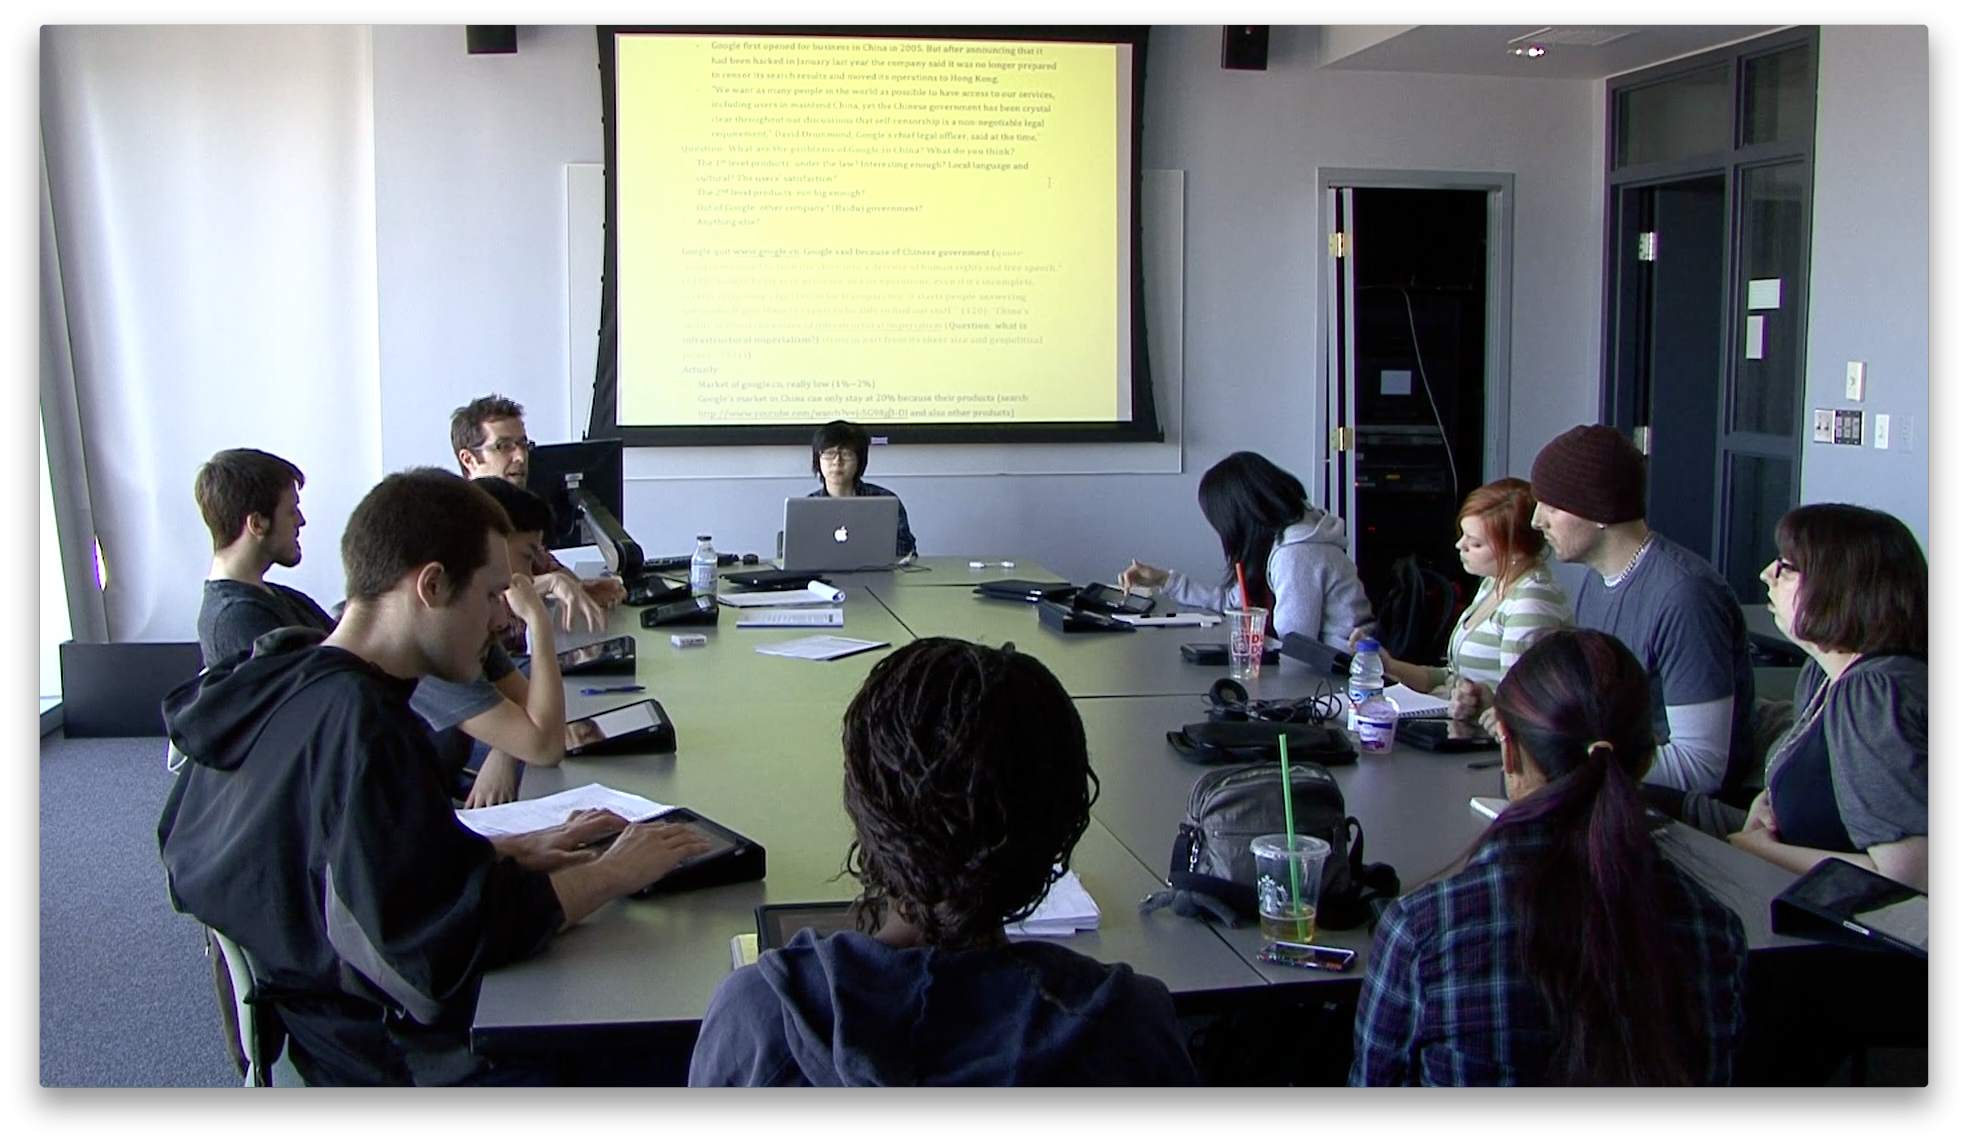
\includegraphics{figures/tincan/classroom_overview.png}
\caption{The classroom environment. The student at the head of the table is presenting and controlling the projector. The professor is to the presenter's right.}
\label{f:classroom}
\end{figure*}

% Commented out, since we're not talking much about the archive to save space.
% \begin{figure}[t]
% \centering
% 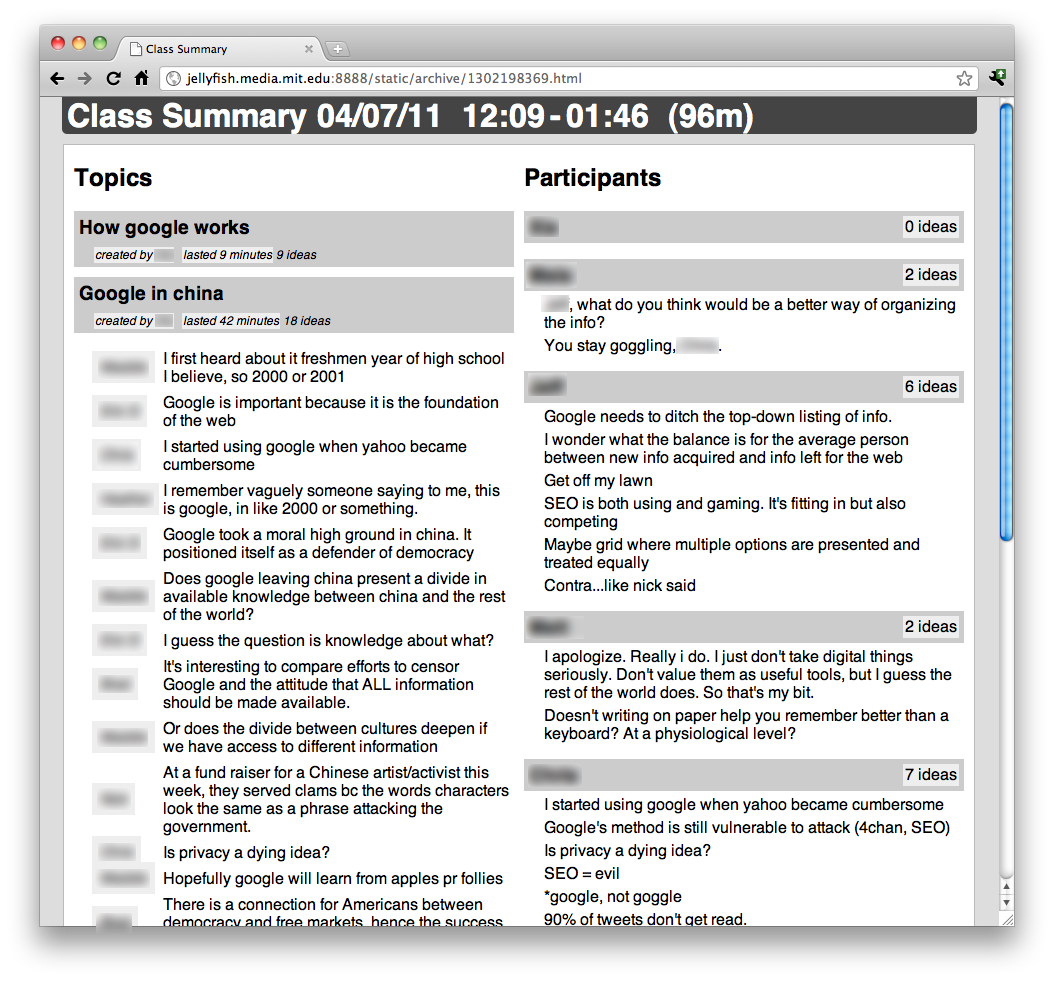
\includegraphics[width=3.25in]{figures/tincan/archive.png}
% \caption{A screenshot of the archive document generated at the end of the class.}
% \label{f:archive}
% \end{figure}

\section{System Design}
 
\emph{Tin Can} is a tablet-based application to support class discussions. It provides a synchronous environment shared by the students and professor and each user has his or her own tablet. Students are physically co-located with the professor. Students arranged their tablet in different ways. Some keep them on their laps, some on the table in front of them. All users (including the professor and researcher) have the same capabilities in the system. The system serves as a visualization of the current state of the group discussion. It focuses on three main parts of a class's process: topics, time, and ideas. Figure \ref{f:interface} shows the interface in action.\footnote{A video of the interface and the classroom context is available at \url{http://www.youtube.com/watch?v=ztVllLuCcTM}}

\subsection{Topics}
The topics pane in the UI collects past, current, and potential future discussion topics. These topics can be added using the ``Add Topic" button at the bottom of the pane. The current topic is highlighted in a topic-specific color. All topics have a short text description. Past and current topics show a kind of clock pie chart, illustrating the start and end times of a discussion topic (or the current time in the case of ongoing topics). The total duration in minutes of past and current topics is also shown as part of the topic text. Topics can be tapped to bring up an interface for changing their state: starting future topics, stopping current topics, and restarting past topics. 

\subsection{Time}
The clock in the center of the screen serves as a reminder both of the current time as well as a concise visual representation of the history of discussion topics covered in the class. The time spent on each topic is swept out radially on the clock such that large blocks of color represent topics that occupied a longer period of the class. When an hour of time has passed, the central area in the clock is cleared and the colored record of the previous hour appears at the edge of the clock. Up to four hours can be easily represented in this way. The clock is non-interactive. 


\subsection{Ideas}
The ideas pane contains a time-sorted list of ideas. An idea is simply a text contribution. Although we had presumptions about what would be posted here (as indicated by the terminology we used in the interface), ideas evolved to include statements, questions, recording main stage discussion themes, and a simple Twitter-like reply syntax. When entering an idea, the author of the idea could do one of two things: ``add idea" or ``add idea to group." The former option would store the idea in the user's ``personal" idea drawer.  The latter option would immediately put the idea at the top of the group idea timeline, as well as adding it to their personal drawer. Users tap and hold to ``like'' an idea. The idea flashes and a ``+$X$'' notation appears in its text, where $X$ is the number of likes that the idea has received in total. Ideas in the group timeline have their author's name displayed in parentheses after the text of the idea. Ideas are colored based to match the color of the current topic. 

\subsection{Users}
Each user logged in to the system is displayed on a tab around the edge of the screen. The arrangement is essentially random. Tapping a user extends that user's idea drawer. This drawer contains all ideas created by the user, whether shared or not. These ideas are differentiated in the list by ``(shared)" being appended to ideas that have been shared. Any unshared idea in the idea drawer can be dragged from the drawer to the group idea area, even if the user didn't originally author the idea. Ideas dragged by other people are attributed differently in the main timeline. For example, an idea created by Alice and shared by Bob would say ``(Alice, shared by Bob)". By design, personal folders are not private.  They are semi-public spaces meant to give users some choice in how their contributions are read by the group.

\begin{figure*}[p]
\centering
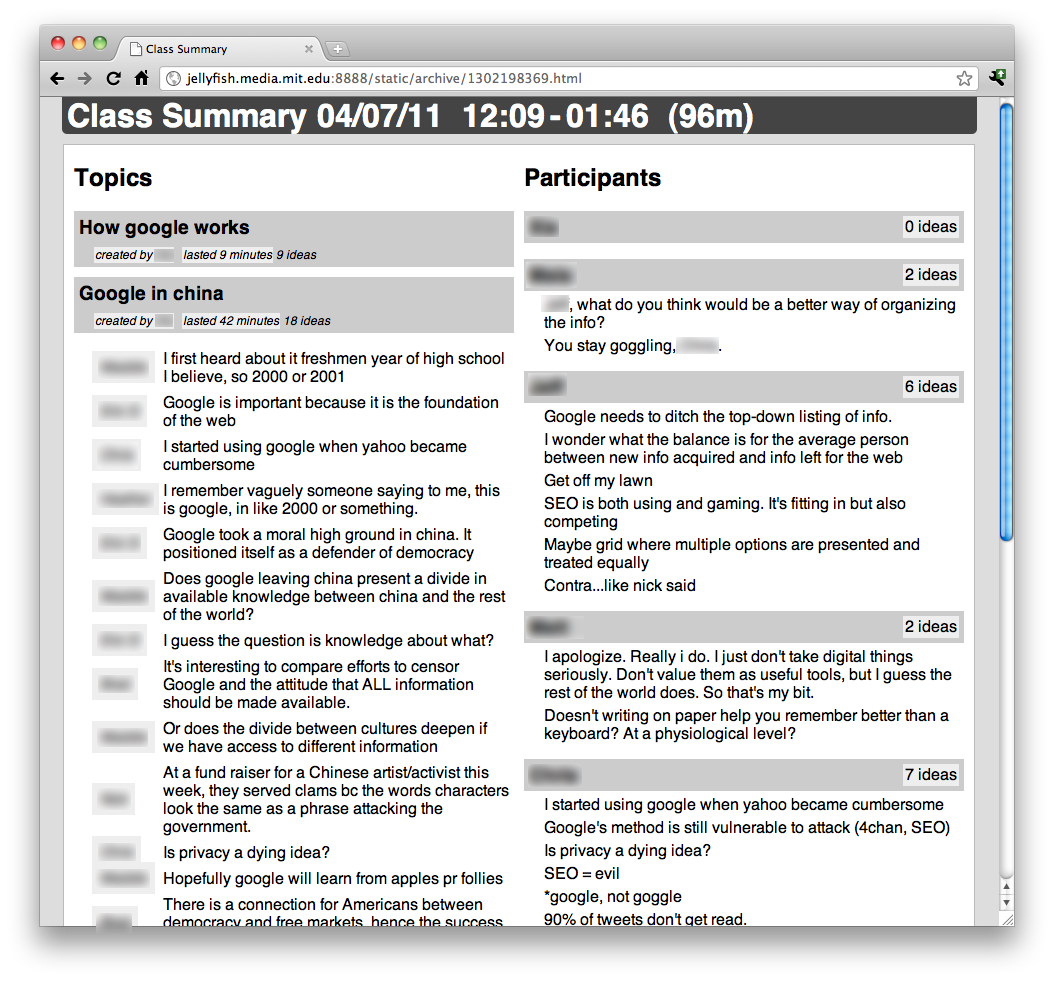
\includegraphics{figures/tincan/archive.png}
\caption{A screenshot of the post-class archive.}
\label{f:archive}
\end{figure*}


\subsection{Archive}
All ideas and topics are recorded on the server. At the end of each class session, the server emails everyone who attended the class with a list of their personal ideas and a link to a shared Web page that include a list of all student ideas sorted by topic and by user.

An example of such an archive is shown in figure \ref{f:archive}.




\section{Research Context and Methods}
We deployed the \emph{Tin Can} system in two sections of a graduate seminar on media and social theory taught by one of the authors \sidenote{Recall that the work of this chapter was a collaboration with Eric Gordon, as published in \citep{Harry:2012df}; he was the professor in this class.} at a liberal arts college. One section met in the morning, the other in the afternoon, twice a week. Class assignments were reading-based. Each discussion class was usually lead by a student or pair of students. While what it meant to lead class changed somewhat over the course of the study, the pre-study norm was to prepare a slideshow and accompanying media (images and video were quite common) and present it to the class. The morning session had eight regular students and the afternoon session had eleven regular students. In total, thirteen students were male, six were female. There were five non-native English speakers in both classes. 

Our study lasted for six weeks and utilized mixed methods, including classroom observations, capture of text inputs, and semi-structured interviews.

Throughout the deployment, user interactions were captured. This did not, notably, include live recording of class audio, only text-based interactions with the \emph{Tin Can} system itself. We made the decision not to record audio because we felt that this would make students self-conscious and would be too disruptive to main stage interactions.  In lieu of audio recordings, for most class sessions, a researcher other than the professor was present to observe the class. We employed a form of direct observation known as continuous monitoring, where the researcher documented everything he saw throughout the study period, including the description of the environment and participant actions, as well as inferences about their meaning \citep{interpersonal_interaction}. The researcher's observations were not prescribed before the study, because of the exploratory nature of this first deployment. We did not know what to expect, so the observations were designed to be generative and not conclusive.  We documented patterns of student attentiveness to peers and professor; interactions with tablets (i.e. position of tablets on the table or in laps); and correlations between speaking and writing. The students were aware that their use of \emph{Tin Can} was being studied and they were aware of the presence of the researcher. Because the students were invested in the use of \emph{Tin Can}, the presence of the researcher was not disruptive, but instead added to the excitement they had about testing a new system.  The field notes were recorded by hand and subsequently transcribed and shared with the teaching researcher. 

All text inputs into \emph{Tin Can} were recorded over 22 hours of usage across twelve class sessions.  Each class was about two hours long, but classes often had a non-discussion logistical content from the professor at the beginning of sessions. The average \emph{Tin Can} session was 105 minutes long. After the deployment, the inputs were categorized into types, including topics and ideas, shared and non-shared.

Finally, at the conclusion of the discussion-based component of the class, the researchers conducted semi-structured individual interviews with fifteen of the nineteen students ($79$\%). Interviews were conducted by the non-teaching researcher to alleviate student concerns about sharing judgements about the teaching researcher, although there were no sections of any of the interviews that students did not want to be shared with the teaching researcher. All interviews were recorded and transcribed and entered into \emph{Dedoose}, a qualitative analysis tool. Because we view this work as generative, we iteratively coded the transcribed interviews, letting themes (and codes) arise organically as we reviewed the interview data, observational data, and process traces from the class. This strategy closely resembles \citeapos{Glaser:1967tj} grounded theory approach. All names mentioned in interviews or shown in screenshots have been obscured or changed to pseudonyms to protect the identities of those participating in the research.

% REVISION Knocked this paragraph out for space. Was just connective tissue and I think we'll do okay without it. 
In the results section to follow we will analyze the kinds of content entered into \emph{Tin Can}.  The discussion section will then connect the interviews and observations to these findings.  


\section{Process Traces}

\begin{figure*}[p]
\centering
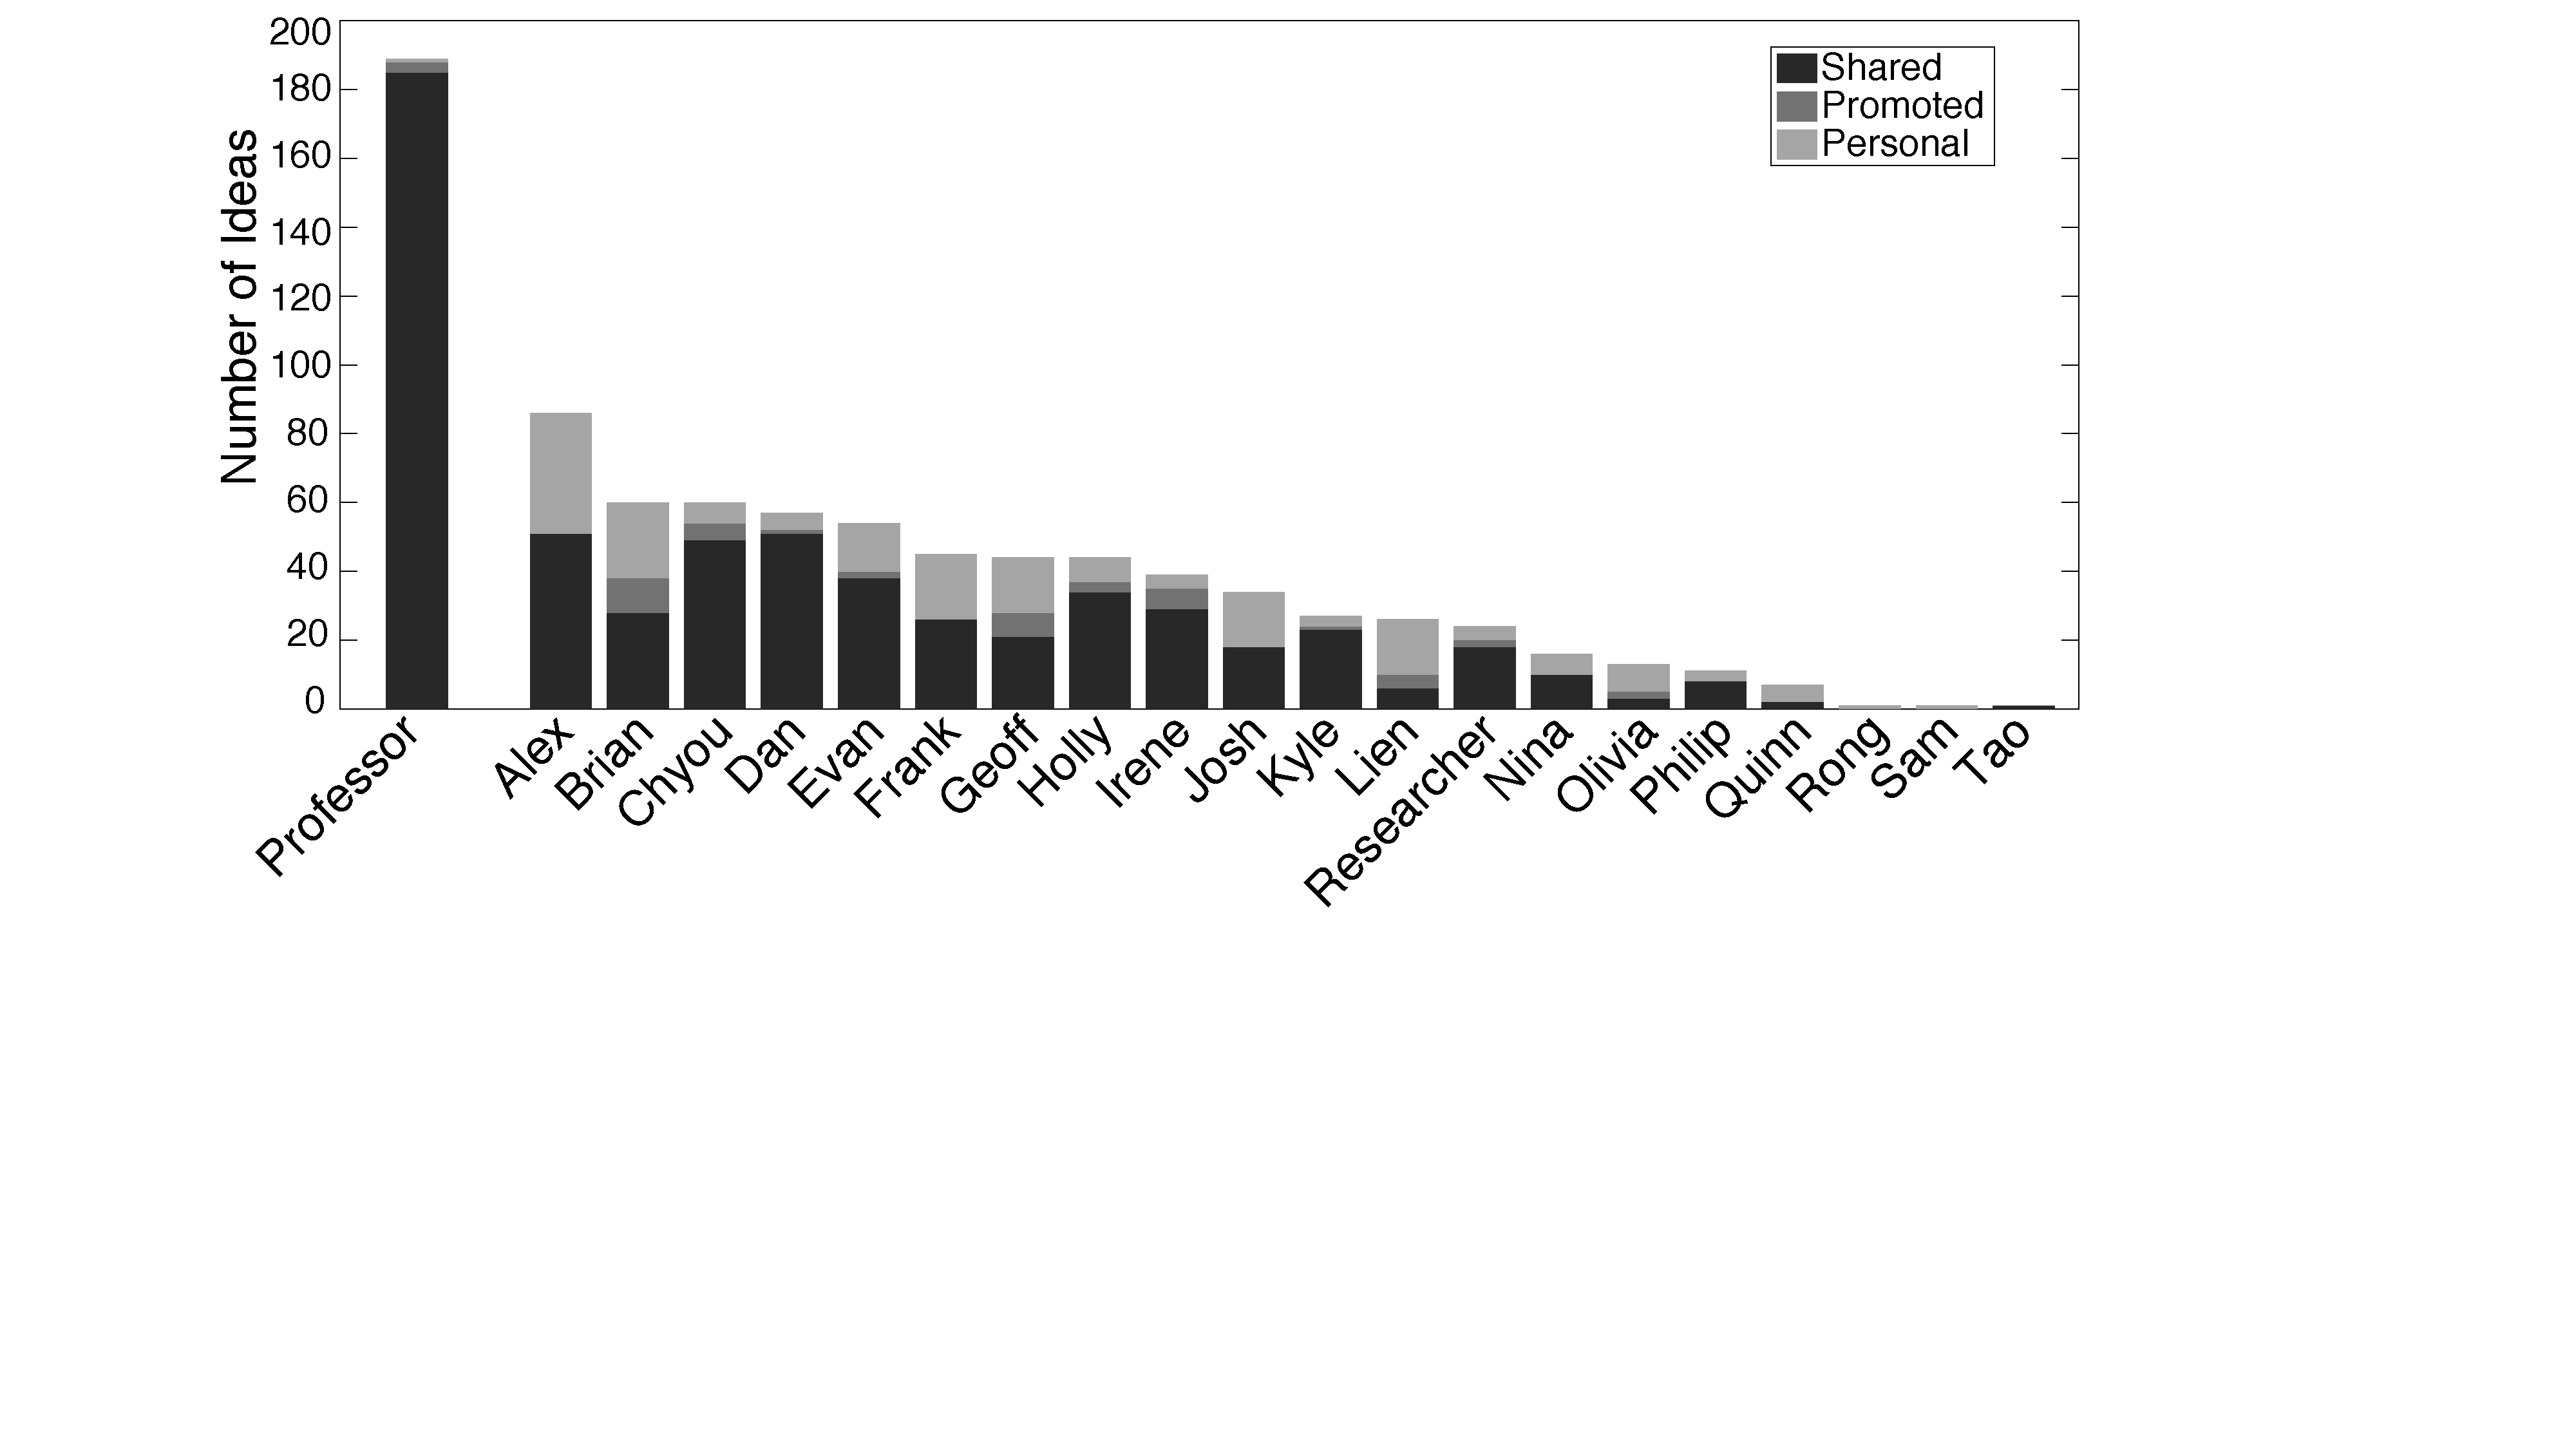
\includegraphics{figures/tincan/ideas_per_participant.pdf}
\caption{Distribution of ideas per participant per idea type: personal, promoted, and shared.}
\label{f:ideas_per_participant}
\end{figure*}

\begin{figure*}[p]
\centering
\includegraphics{figures/tincan/timeline.pdf}
\caption{Timeline of topics and ideas posted in two example class sessions. Ideas posted by students are in black, ideas from the professor are in red. The height of the line indicates the length (in characters) of the idea. Topic names are shown above their corresponding section of the class.}
\label{f:class_timelines}
\end{figure*}


Over the course of the deployment of \emph{Tin Can}, 839 ideas and 119 topics were created. The  majority of ideas created were shared: $72\%$ of ideas were shared on creation. Another $5\%$ were personal ideas that were turned into public ideas by being dragged by another user from a user's personal idea drawer to the public idea area. The balance, $23\%$ of ideas, were never shared. The distribution of these different idea types on a per participant basis can be found in figure \ref{f:ideas_per_participant}. 

Over the course of the study, 119 topics were created in total. Of these, 79 were actually discussed and the remainder were raised as potential topics but never actually used. The average class had 6.5 started topics, with a standard deviation of 2.3. Topic duration had a much wider variation: the average topic lasted 851 seconds with a deviation of 673 seconds. This is skewed largely because of very short topics. 

A deep analysis of temporal patterns within the data is beyond the scope of this paper, but to provide a rough sense of what topic and idea posting activity looked like we have provided two example timelines in figure \ref{f:class_timelines}. The most striking thing about the data from this perspective is that the temporal distribution is very uneven. In Kleinberg's terms, we see a bursty structure \citep{Kleinberg:2003ej} in idea posting. This is a common structure in communication systems and it is no surprise that it appeared in our study results. 

% REVISON I don't think we need this. In what follows, we present some summary statistics of topic and idea use during class, discuss some of its temporal properties, and describe a rough set of categories that capture the diversity and relative frequency of student ideas in \emph{Tin Can}.





%WHAT WOULD YOU SAY ABOUT CUTTING OUT THE ENTIRE IDEAS SECTION? I'M NOT SURE IT IS NEEDED.
%REVISON I don't think we need this sentence. We intentionally provided little guidance, beyond the name itself, for what the ideas section of the interface was intended. 


\subsection{Ideas}

Over the course of the semester, ideas were adapted for many different purposes. Based on a review of the captured ideas, we organized them into a set of broad categories.

Statements were the most common type of idea. Statements capture an argument or idea, like ``Talking about sex is a means of controlling it.'' These contributions are similar to what someone might say if they had a speaking turn. Alternatively, they sometimes represented note-taking behavior. Students were also particularly fond of ``X vs Y'' dualisms, which we describe as Theme ideas. Like statements, these often had a dual purpose of either proposing a useful dualism or capturing the nature of the current discussion. 

Questions were about half as common as statements. They usually took a rhetorical form, like ``Where do you draw the line between not being sexually repressive and being excessively open about it?'', or were framed as less forceful variants of statements like ``Is identity a sign? Or is it that which is signified?''

Early in the study, students developed techniques to address their ideas at specific other students. Using ``@'' syntax, as in ``@dan, I don't think the two are mutually exclusive.'' they could respond to other students' ideas non-orally.


\section{Discussion}
Much of the existing literature on backchannels focuses on situations in which the audience has one stage to perform on and the presenter has a separate one.  \citep{Yardi:2006uk, mccarthy_digital_2004} \emph{Tin Can}'s symmetry, where anyone can use either stage at any time, is the focus of our analysis. In this section, we use the stages metaphor introduced earlier to describe how students managed their attention to stages. Then, we discuss how students made decisions about when and how to perform on the available stages. 

\subsection{Attention}
% Attention, for our purposes, is best understood not as an innate characteristic of someone's behavior, but as a value-laden socially situated performative behavior. ``We are always to a certain extent in a state of distraction,'' according to sociologist Emile Durkheim. \citep{Durkheim:1974tc} Every situation is composed of stimuli that disrupts some fictional conception of undivided attention.  Likewise, every situation requires some aspect of performance, as individuals are required to communicate their attentiveness in response to specific social contexts.

As described in Chapter \ref{ch:background}, attention is best understood as a socially situated performative behavior. In a lecture, attentiveness is typically demonstrated by looking at the presenter and potentially taking notes. In a small group discussion, attentiveness might be expanded to include looking through class reading material or looking at other people. 


Traditional approaches to managing attention in education tend to take as their starting point the desire to maximize audience attention on the presenter through the physical architecture of lecture spaces, presentation media, and rhetorical strategies. \citet{Gordon:2009us} argue that attention and distraction are best understood as being ``hand-in-hand. The very same new technologies and landscapes that cultivate a state of distraction are themselves directed simultaneously toward the cultivation of attention.'' Educators tend to look to technology (broadly construed) to help manage overwhelming sensory inputs while simultaneously blaming the lack of attention of students on that same technology.

% cite giddens here? I do love the structure + enactment stuff, but I'm not sure it's something we can just drop in here unless it's other places too and gets a paragraph introducing it to people who might be unfamiliar with it. 

Of course, it is not simply a definitional matter to decide what constitutes attention in a class using \emph{Tin Can}. To understand how students and professor understood attention in this context we can look to how they talked about attention and distraction. Students predominantly viewed participation as obligatory. Speaking to his motivation to use \emph{Tin Can}, one student said ``to be part of the class I had to use it.'' Students were never admonished for interacting with tablets, and didn't report feeling like they needed to minimize their performance on the side stage to avoid negative perceptions of themselves by the professor or others, except to the extent that students felt like over-participation on either stage might crowd out other students. A student who was particularly active on the side stage worried that ``I take so much space that people that are shy...have more problems ... standing up when they have personal ideas [to share].''

%QUESTION: is that quote above accurate?  It doesn't make much sense?

To the extent that students were concerned with attention, the most common problem was not being viewed as inattentive, but struggling to track performances on both stages simultaneously. Although students were not concerned with annoying the professor, they were worried about offending their peers who were presenting that day: ``It is a little tough to keep your attention on both [stages], and sometimes you get a running conversation on \emph{Tin Can}, which can be interesting but it is maybe a little unfair to the presenter.'' Although this perspective represents a pull towards enacting traditional models of attention, it wasn't enough to significantly diminish involvement (either as a performer or an audience member) on the side stage. Student presenters often used \emph{Tin Can} as a way to gauge interest in future discussion topics and to decide on whom to call.

In resolving the conflict between compelling simultaneous performances, students could fall back on the persistence of performances on the side stage. In making a choice to attend to the main stage, they could, in Josh's words, ``have a comfort that you're not going to miss anything because you can always go back and see other people's posts whenever.'' Still, there seemed to be a difference between browsing posts later and being part of the live conversation. This came up most frequently when students expressed frustration with text entry on the tablet and missing the right moment to post something: ``I didn't get it out as fast as I'd hoped and it was already passed and it wasn't worth typing it anymore.'' 

%Although posts would be available for reading later, there was still a sense of timeliness and not attending to the side stage represented a sort of sacrifice of opportunities for performance. 

% TODO could chop that last clause, I guess.

Deciding between stages was really only a problem when both stages were compelling. If only the main stage was compelling, students could freely attend to that. The reverse was also common, and students frequently reported attending to the side stage as an escape from an un-engaging main stage, as in this quote from Quinn:
\begin{quote}
``I can remember a particular ... presentation that he was doing a lot of PowerPoint, I think he was completely oblivious to the \emph{Tin Can} conversation and [the \emph{Tin Can} conversation] ended up going in a very good direction ... as a result, I do not remember anything he said, because ... the conversation on \emph{Tin Can} was a little more engaging''
\end{quote}


% REVISION I want to make this point somewhere, but I'm not sure exactly where to do it. I sort of what it earlier, but if it's before the performative attention argument it might feel a little adrift. 

%This is great.  I like the paragraph here.

Moments like this highlight the extent to which our characterization of stages as ``main'' and ``side'' is itself a product of attention. The presence of a system like \emph{Tin Can} does not automatically create a side stage, nor does the ability for spoken communication guarantee that such communication will create a main stage.  The addition of a mediated communication platform simply creates the \emph{possibility} of a new stage. Whether or not it becomes a viable stage, and whether the mediated stage is a main stage or a side stage is all the result of people's attention to and actions in the system. Furthermore, the designation ``main'' or ``side'' is not fixed. The situation Quinn describes is a moment where the main stage ceased, for a little while, to command people's attention and \emph{Tin Can} took on some main stage properties. Although such moments were rare, they point out how stages are not created by technology or decree: they are designated and sustain by the collective attention and action of people using them.


The professor's high level of activity on \emph{Tin Can} throughout the class can be seen as playing a role in setting the main/side distinctions. His activity was a way of giving students permission to take the side stage seriously, both because it was clear that he was going to notice contributions from students, but also because he was frequently entering ideas himself and not looking at the current speaker. This underlines the extent to which this was an ideal context for testing a system like \emph{Tin Can}. Had we deployed in a class where the professor was neutral or hostile to people attending to \emph{Tin Can}, traditional class expectations of attention would more likely have been practiced by students, reinforcing those norms and making a side stage much less viable.




% I think I want a paragraph here about how the professor viewed attention, but not sure how to attack it. I want to say something about how the professor's high activity level + framing of participation on TC as "part" of the class as playing an instrumental role in expanding the boundaries of potential attentive behavior. I think we can see this in the "role of the professor" codes. People talk about viewing participation as "mandatory" or "expected", which I think suggests that they had explicit permission from you to see use of the system as part of positive participation. 

% not sure if we want to include this, but figured I'd spit out a first pass paragraph for it.

% This is a nice story, but I don't think we have room for it here. 
% -----------------------------
There was a moment towards the end of our study when the professor brought in a colleague over video chat to discuss his work and answer questions from the class. The remote presenter had a very limited view of the room from the professor's laptop video camera and could see only a few students. Although the \emph{Tin Can} system was available for this section of the class, it went almost entirely unused. This may simply be because the activity on the main stage was engrossing, but the total lack of side stage performance was still well outside of the bounds of normal disuse during a particularly engaging presentation in class. This suggests to us that the students were concerned with enacting the traditional model of attention for this outsider to the class. He could have viewed intense tablet use (something that was normal and viewed as attentive during normal class sessions) as inattentive or disrespectful and so his presence (even though his view of the classroom was quite limited) triggered a reversion to the more restrictive expectations of attention in a traditional class context.

% I like this too, but this doesn't add a whole lot and isn't that strong.
% -----------------------------
During class sessions, we also conducted focused observations of student attention. The researcher would pick a student and mark down when they changed what they were looking at. Although this was not comprehensive data for all students, when students weren't looking at the current speaker they were predominantly concerned with their own bodies and clothing, not the tablet. The tablet hardly dominated their attention. Even among the most active users of \emph{Tin Can}, their attention was usually on the speaker and shifted to the tablet during periods of silence or topics they found less interesting. When the professor spoke, students were far more likely to look at him than when other students were speaking. 

\subsection{Performance}

The presence of an additional participation stage complicates the experience of being a member of the class. When should you submit an idea on the tablet rather than say it out loud? When is the right time to say something? Should you share an idea or make it a personal idea? The enacted (and self-reported) answers to these questions can provide some insight into the experience of using the system as well as deepen our understanding of the stages metaphor. In many cases, students viewed the side stage as complementing the main stage and valued its presence in situations where a range of problems with the main stage impeded their participation. In this way, \emph{Tin Can} acted as a kind of escape valve: when the main stage was working for people, they used it; when they felt like they could not use it or did not want to use it, they turned to the side stage and valued its complementary affordances.

Performance on the main stage was widely viewed as more challenging and having higher stakes than side stage performance. Among the students who were reluctant oral participants in class, this was particularly acute. Geoff, a very rare oral participant in class before \emph{Tin Can}, was particularly frank on this point: ``I don't really talk a lot in class because I'm scared of sounding stupid.'' Geoff was a more frequent side stage participant. Although he would still rarely speak up directly in class, he was often called on by others in class to speak about ideas he had posted on \emph{Tin Can}; he would happily speak in those instances. This change in behavior on his part was frequently brought up by other students as being a major benefit of using \emph{Tin Can} because they valued the opportunity to hear and see what he was thinking. Irene, a more talkative student, characterized Geoff as a member of a ``good chunk of people who I think are thinkers and they would just think and write down what they were thinking'' as opposed to speaking on the main stage. This feeling was common among people who were comfortable on the main stage, who acknowledged that ``not everyone feels comfortable speaking in class, so I think [\emph{Tin Can}] definitely allowed for certain ideas to be shared that probably would have been either suppressed or just ignored or forgotten.''

Students' comfort with the different properties of the main stage and side stage influenced which stage they chose for a performance. Students for whom English was a native language were more comfortable in spoken conversation, and when faced with complex ideas preferred to express them orally, turning to \emph{Tin Can} to express simpler ideas because typing complex ideas was slow. Students who did not speak English natively had the reverse logic, preferring to type complicated ideas so they could, according to Rong, ``organize my language a lot before I actually talk because I want my thoughts to be systematical and clear, I want people to get it.'' In both groups, though, students viewed the revisability of written contributions as a potential benefit: ``[\emph{Tin Can}] gave me the advantage of thinking it through in a writing sense a little bit before I vocalized the idea.''

A lack of confidence about one's performances was not the only reason to choose the side stage over the main stage. Students had a clear sense of etiquette surrounding when they could participate on the main stage and in what ways. Because only one person could be talking at once and conversations were fundamentally linear, students often felt like speaking up themselves would be changing the flow of the conversation in an inappropriate way. Instead, students would prefer to write their comments on the side stage instead of ``interrupting'' on the main stage. This was intertwined with ideas of timeliness. Performances seen as being closely related to the current main stage conversation were more appropriate than performances that might drag the conversation in a significantly different direction. Although similar, these concerns are not precisely the same. The worry about interruption was primarily a desire to not unduly influence the path of the conversation because that was perceived by some students as the role of the professor or presenter, not the role of the individual student. In contrast, ideas that were seen as ``not quite as relevant [and not] really [fitting] into the conversation'' were not really valid performances on the main stage at all because not only would they move the conversation significantly, they did not necessarily have anything to do with the existing main stage conversation.

Both of these worries, though, led to the same thing: increased use of the side stage. Because turn-taking was not a concern on the side stage, it easily supported ideas going in different directions simultaneously. To the extent that those directions were interesting to other people, they could serve as the basis for future ideas. If they were not, it was not seen as problematic to have put them there in the first place. When an idea did not seem to lead to any future ideas, students ``didn't think anything of it. Not all ideas are great.''

% There's a side point here that we can probably leave behind, but just to keep it around... There is an interesting thread of comments where people talk about missing out on the activity on the side stage. This is surprising because we also have people talking about how nice the archivability is beacuse they can always come back and look at it later. There's something really subtle here about how there is still a sense of the side stage being ``live'', but it doesn't seem to suffer from concerns about distraction. Even though there's a sense of where the conversation is now on the side stage, no one worries about changing the state of that conversation nearly as much as they do on the main stage.

% the difference here seems to be between the more talktive people (like a heather) and less talkative (like qinshu). more talktive 


%``if this was something I thought was really current and in the moment I would say it out loud and you know I didn't care about the community but if it was something that was not quite as relevant it doesn't really fit into the conversation, maybe just put it in''

%``It can be frustrating with any kind of class when you have something that you want to say but you know there's a lot of other stuff going on and it might not even be appropriate for a time, maybe it was something you've already done or you haven't gotten to it yet but if you weren't marked down an idea to be brought up later.  So yeah I think that's useful. And also to see what everyone was was thinking, if they're on the same page.'' (both matt)



\subsection{Sharing and Promotion}

Key to our argument about stages is moving from a model where we view people as ``tuning in'' to a single channel to one where we recognize that computer-mediated communication systems offer new simultaneous stages on which we can perform and be observed. It is critical, then, that we describe how performances shifted between stages, influencing what students said and how they said it. One common pattern was the positive reception to ideas on the side stage encouraging those ideas to be performed on the main stage. This same process happened even within \emph{Tin Can}, when personal ideas were dragged by someone (usually the professor; $57\%$ of ideas promoted from personal to shared were promoted by the professor) to the public idea timeline. Students also viewed ``likes'' and replies as good indicators of interest in their ideas. Geoff, the quiet student discussed earlier, captured the impact of these promotions nicely: ``At first I started just putting them in my box [i.e. making them personal ideas] without even sharing with the class. Then I saw that [the professor] started dragging them out and putting them in discussions so afterwards I was more open to sharing my ideas within the class discussion.''

Activity on the side stage was sometimes explicitly moved onto the main stage. In most cases, the professor or student presenter called on someone based on something they had said on \emph{Tin Can} and asked them to re-perform the idea on the main stage. The professor might say, for instance ``Olivia, you had a nice point here on \emph{Tin Can}, do you want to expand on it?'' and Olivia could elect to take a speaking turn (and nearly always did). The other common strategy was for a speaker (particularly a student presenter) to use an idea recorded on the side stage as a starting point for a comment of their own or to introduce a topic known to be of interest to students based on side stage activity. Promotion moves by the professor were valued over those by other students, but both were appreciated and clearly remembered by students. 

Part of our goal with the system was to use participation on \emph{Tin Can} as the basis for an archive. Students were aware of this goal, and it was reinforced by the emails they received after class with a link to the shared class record of topics and ideas generated in class. Students occasionally talked sometimes about their ideas as an attempt to ``take notes'', but more often they viewed that as the professor's role. Not, perhaps, because it was a natural role they \emph{a priori} expected of him, but because it captured (in their view) his observed usage.

In the stages framing, we can understand note-taking as moving performances from the main (oral) stage to the side (text) stage. For example, these were ideas entered into \emph{Tin Can}: ``Play is no longer having fun, it is work'', ``Question of self-efficacy in public sector'' or ``Consumption leads to feeling good about yourself.'' When posted by students, ideas of this form were frequently attempts to move the discussion, but when they were posted by the professor they were seen as records of the main stage. Students characterized the professor's role in this process as ``the note taker person so if ... the presenter said something [the professor] would summarize what they just said.'' This was seen as a valuable contribution by the students that showed interest in reviewing the archives after class: ``I liked the way [the professor] used it. Because that also meant that I didn't need to take notes ... because he posted it in \emph{Tin Can} and I could get access to that later.''

% REVISION This is a good place to talk about try-marking, I think. Some early text for that:
% We can, therefore, think of these side stage contributions as being implicitly ``try-marked'' in Sacks and Schegloff's terms \cite{Sacks:1979vo}. If they were promoted 
% Because ideas presented in \emph{Tin Can} didn't require acceptance by anyone due to the nature of the system (e.g. a lack of an acceptance move from )
% Will have to wrestle with what point, exactly, we're trying to make here. 


% REVISION Could write something here about how this mirrors findings from Livenote, although livenote is a little bit vague on this point. I think it's a fair characterization, but they don't make a big deal of it at all. 

As is evident from figure \ref{f:ideas_per_participant}, the professor was a significant outlier in terms of his performance on \emph{Tin Can} and his participation clearly had a big impact on how students understood and used the tool. Beyond his role as a note-taker, students also viewed his performances as oriented towards trying to guide the main stage conversation in particular ways. Students characterized this use pattern as, variously, ``guiding'', ``influencing'', or ``driving.'' He was particularly interested in ``[initiating] conversation'', primarily by posting thought-provoking questions like ``Why do we feel responsible for a corp's feelings?'' or ``What is the role of god in modernism?'' Most students avoided starting or stopping topics (or proposing them at all), arguing that it was the professor's job to do that, although some students took more active roles in administrating topics when they were in the presentation role. In total, $53\%$ of topic-related state changes were done by the professor. 

On the main stage, the professor was also a frequent promoter of side stage activity. Sam characterized the professor's role in a particularly evocative way:

\begin{quote}
``I feel like [the professor] would be a speaker for people who couldn't speak, you know.  The fact that he was really into \emph{Tin Can}, so he would read something that [a student] had written and be like oh, I want to quote this or talk about it and [act] as a spokesman for people who aren't really comfortable speaking''
\end{quote}

This underlines the professor's role as a bidirectional bridge between the stages. By taking notes on main stage performances, he reinforced \emph{Tin Can}'s note-taking role. By speaking out about side stage performances and drawing people into the discussion based on written ideas, he legitimated their side stage performances. It is very hard to imagine \emph{Tin Can} being as well integrated into the class as it was without the extensive involvement of the professor. This does not, in our minds, diminish the contributions of this work. Although we cannot speak to how a skeptical professor might react to the system, having a fertile classroom situation gives us an opportunity to make important insights into the potential for this design space that we might not have otherwise been able to access.

%QUESTION: Is this last paragraph redundant?  I seem to recall we say something similar someplace else?


\subsection{Hardware}

While one could easily imagine \emph{Tin Can} working on a laptop, its deployment on tablets substantially affected use and outcomes in a variety of ways. First, there is a simple visual benefit to using tablets. Unlike laptops, which can create strong visual boundaries between people, tablets lie flat (or nearly flat) on the table or in people's laps. When organized around a rectangular seminar table, tablets do not disrupt sight lines between people. In general, laptops give people something to hide behind while tablets more strongly signal availability.

Accordingly, tablets offer less privacy than laptops. Participants can easily see when other participants are using the system, and typing is easily distinguishable from browsing other people's ideas. Surprisingly, we frequently saw students looking at other students' tablets while they interacted with them, even though everyone's view of the space was the same. Students seemed to be interested in knowing how other people were using the system. 

Because of the way the tablet program was administrated at the school, students did not have any particular ownership over a specific tablet. This inhibited any sense of ownership; students talked about the tablets as being essentially disposable, for example ``sometimes the [tablet] would run out of battery and kick you off and you'd have to get a new one.'' The benefit of this lack of ownership was that it limited the tablets' non-\emph{Tin Can} uses. Unlike a laptop, on which the Web and communication tools were a click away, the tablets were not personalized. Even using Web tools was tedious, because they had to log in to each one which was both slow and obvious to people around them. 

The biggest challenge with tablets is data entry. The most frequent complaint about the system was how slow and difficult they found accurate text entry to be. Students complained about slow typing speed making it hard to post timely ideas (``I didn't get [an idea] out as fast as I'd hoped and it was already passed and it wasn't worth typing it anymore'') and distracting them from the main stage (``it takes time to type on the [tablet] and so probably it takes you away from the presentation sometimes''). We also saw a number of ideas correcting typos and autocorrect mistakes in previous ideas. These problems mitigate the system's utility as a conversational stage and seemed to depress overall use.


% This section needs a new title. I sort of want to call it conclusions, but that's unconventional. Traditionally conclusions just repeat the main findings of the paper. I sort of hate that style, but it's not traditionally a place to make new points. We could also call it "analysis" or something, but traditionally those sections happen before a discussion section, not after it, and I don't think it really captures what's going on here. Ultimately, given how tight a paper this is I'm leaning towards calling it conclusions, slimming it a little bit and nuking the existing conclusions section. But I'm going to sleep on it. 

\section{Conclusions}

% this subsection feels ripe for cutting to me. 

In deploying \emph{Tin Can}, we had two major goals: increase the diversity of participation and increase engagement.  We feel that we were successful in each of these goals.

When judging participation, we consider activity on each stage. In terms of the main stage, we saw some evidence that people who might not have spoken up in class were prompted to speak by \emph{Tin Can}. Most often, this came from the promotion processes described earlier. This moderately increased the diversity of participation on the main stage. Side stage participation was viewed by both students and professor as a legitimate way to be a class participant, and we saw much broader participation in \emph{Tin Can} than we saw on the main stage. The distribution of side stage participation was relatively flat, setting aside the professor, especially  when compared to the steep power law reported in a chat backchannel \citep{Yardi:2006uk}.  Based on our discussion of how and when students chose to participate, it is clear that the distinct affordances of the main stage and side stage meant that each captured kinds of participation that would not have been effective on the other. It is not the case that adding \emph{Tin Can} detracted from the main stage and that there is a simple conservation of participation across all formats; we saw a more subtle case in which having a communication outlet with different properties drew out contributions that otherwise would not have happened at all.

% what does 'engagement' really mean in this context? What were we hoping for? I think need to confer with Eric about this paragraph before writing it. I think in some ways this is an anti-distraction thing? Like, we're worried about people not paying attention to things? We have some data about students using the tool to reground themselves in the conversation, but I'm not totaly sure how to make an engagement argument or on what basis. Maybe the way to slice these three goals is to say: diversity, overall participation, archives? Not sure I like it, but the first two issues are more or less covered in the paragraph above and could basically leave it at that. 

We found little evidence of students making use of the archival records generated by \emph{Tin Can}. The presence of the system did not, as we hoped, encourage students to participate on \emph{Tin Can} because it generated a shared record of the class. In practice, students referred to the archive infrequently, and rarely reported that it influenced the kinds of ideas they wrote or how they wrote them. Although the archive was not frequently used, it did prove useful to some students. One student, Lien, valued the presence of the shared archive because ``it [took] the pressure off of me. I don't have to write down all of the notes.'' Frequently, students said they had stopped taking written notes in favor of relying on the archive instead (even if they subsequently did not access the archive). Perhaps the lack of access should be seen as unsurprising because students may have been just as unlikely to review their own notes. Also, it may be because the course was a humanities-style theory course with a research paper and no final exam, students did not view the material as additive.  If it was deployed in a skills-based course with more incentive for review, the archive may have played a more central role. Still, we were disappointed that it did not seem to motivate participation or reflection outside class. 

% is it possible to find a cite about student lookup of old notes? would be neat to find something to compare against here.

This system was consciously designed for students who were less likely to participate orally in class. We were surprised at the extent to which attitudes about the system aligned along active oral participant / reluctant oral participant lines. Active oral participants tended to be indifferent about how \emph{Tin Can} affected their personal participation in class. However, they acknowledged its effect on less active participants.  Members of this group almost always commented on the increased diversity of involvement that \emph{Tin Can} promoted, with observations like: ``it tends to be a certain group of people who would talk and a certain group of people who were thinking but not talking. So I would like to see what they were up to.'' Philip, an active oral participant with essentially zero \emph{Tin Can} participation noted of reluctant oral participants ``maybe [reluctant participants] would have something to say but maybe there's like some sort of reluctance to actually to speak the thing aloud. So it gave another sort of channel to express ideas.'' Knowing that reluctant participants had a place to participate made active participants feel less guilty about their own participation on the main stage.

Reluctant oral participants broadly relished the opportunity to participate in new ways with which they were more comfortable. Students described the system as ``more efficient'', it ``gave more people a chance to say things that they wouldn't say'', and it helped students ``feel more connected to the other students.'' Olivia poignantly described the system as ``something that was on my side, so to speak. You know what I mean? ... Like it was a resource.'' 

% REVISION Could we add a little heft here to make it clearer how much reluctant participants liked the system? Perhaps we're being unneccessarily coy about how strong the results are here.

% Added this paragraph in to tie back to Second Messenger.
This dynamic between reluctant and active main stage participants suggests a new view on \citeapos{DiMicco:2007ie} findings. They found that although visualizing participation decreased participation among over-participators, it did not boost participation of under-participators. In contrast, we found that although \emph{Tin Can} did not decrease oral participation among active oral participants, it \emph{did} boost oral participation among reluctant participants by letting them try out potential comments in a less intimidating medium and gather support for those ideas before speaking about them to a wider audience. Furthermore, if we include non-spoken participation, reluctant participants increased their participation substantially. This suggests that a lack of participation is not simply an issue of under-participators not finding conversational space to jump in, but can represent low conversational confidence that needs to be specifically addressed to boost participation.

% This may not be valuable, I just was thinking about it and thought I would put it in and see how it felt. It definitely does help link findings better, which is something we were lacking.

%I love the new paragraphs.  They nicely tie our conclusions together.  In fact, we might consider moving them to the conclusion.

We can also compare this boost in participation to \citeapos{Bergstrom:2009ej} finding that under-participators on the oral stage were also under-participators in voting. Our findings suggest that if participation rates are strongly correlated, perhaps the votes do not represent a different stage. This would fit with \citeapos{Tatar:1991jq} findings with \emph{Cognoter}; although \emph{Cognoter} had more communication opportunities than \emph{Conversation Votes}, participation in \emph{Cognoter} nonetheless frequently stalled audio conversation while discussants processed the contribution. Simply providing another communication venue does not necessarily create a stage. 

Our findings are also surprising in light of \citeapos{Tatar:1991jq} analysis of the ``parcel-post'' style of communication. Although it would be fair to describe ideas in \emph{Tin Can} as parcel-post, we did not observe any of the breaks in main stage participation resulting from submitted ideas that were observed in \emph{Cognoter}'s use. Students frequently talked about waiting to read ideas when there was down-time on the main stage, something Tatar et al. view as a central problem with the parcel-post model in a face-to-face environment. We suspect that the main difference is group size. At small group sizes (like Bergstrom's table-based work and the \emph{Cognoter} studies) it is quite difficult to maintain separate stages because participation on the side stage is so conspicuous and attracts immediate attention. In Goffman's terms, it is a venue where it is difficult to ``get away with going away''. At larger group sizes like those we observe in this work, it is difficult to constantly participate on the side stage (either as a reader or a writer), so immediate awareness or consideration of all side stage contributions is simply not feasible. In fact, this lack of obvious immediate attention on each contribution could be a big part of why reluctant participants were more comfortable making side stage contributions. 

% REVISION I think I'd be okay dropping this paragraph. We're just saying "wellll, we can't say this made people learn better but we think it does anyway and you'd need a real study to answer that question." I guess we're covering our asses on comments asking about educational outcomes, but since we never talk about them anywhere, I'd be fine not talking about them at all here, either.

% Although it is difficult to argue about educational outcomes based on a study like this one, we think that the system's broad appreciation among both major groups of students is a sign that the system at least crosses the threshold of ``useful'' and met most of our major design goals. Whether broader participation and increased engagement improve educational outcomes is beyond the scope of this work, but we are encouraged by our observations and interviews with students that use of this sort of system could have a significant positive educational impact. Measuring that kind of effect would require a broader deployment and controlled experimental structure.

%``it's more efficient than the traditional wavelength where you raise your hand and say your idea, and it's definitely an improvement.'' (Chang)

%``definitely made us less afraid to speak about things, which is good. I feel like it definitely gave more people a chance to say things that they wouldn't say.'' (Elizabeth)

%``I wish we were still using it. I had some stuff to say but again I don't want to sound stupid.'' (Eric V)

%``in some ways you do feel more connected by the other students, like especially I can imagine in a class like if you don't know everyone how that can be a class that you just sit there and ignore everybody and otherwise it would be a boring class and you'd just sit there and not know anyone'' (Matt)

% not sure exactly what to cite here, but could do artifacts/politics or something out of the management literature I've been reading lately. 

%We were most gratified to find that students in that position found the system to be particularly meaningful. 

%`` I think what it came down to was that even though I didn't use it, it felt like it was something that was on my side, so to speak. You know what I mean? That's kind of a weird way to put it. You know what I mean? Like it was a resource, I guess.''

%``So \emph{Tin Can} was a good you know kind of forum to dump ideas where people would help to kind of get a conversation going and actually it was a good kind of catalyst for that.'' (Nick)

% ``I think that the discussions we had with \emph{Tin Can} were a lot more fruitful than the ones without it. I think that a lot of the discussions we had with \emph{Tin Can} were better than the ones without.'' (Ross)

 % also can do some suggested changes, based on our findings. eg ways we wanted to make it better but didn't have time to do. 


%In this paper, we described the design of a tablet-based application that creates a synchronous space to share ideas, manage topics, keep track of time, and generate a shared record of the class. We conducted an extensive deployment of the system in a seminar-style class and collected process traces from use, recorded observations of the class process, and conducted post-deployment interviews with students in the class.

Based on our study, we conclude that the introduction of a tablet-based system into a seminar classroom can have positive effects on the engagement of students and diversity of their participation without sacrificing the primary mode of interaction: spoken conversation.  Unmediated face-to-face group discussions can be high pressure situations.  Participating in face-to-face discussions requires participants to perform ``live'' (performances cannot easily be composed in advance); they also typically come with predetermined notions of etiquette to which one must adhere in order to preserve the integrity of the performance. We wanted to design for this context in order to take advantage of the rich texture of participant attention and performative attributes the seminar setting presents. Our study demonstrated that \emph{Tin Can} gave a voice to students who otherwise were not confident enough to perform on the main stage or who needed to ``test out'' ideas before sharing them on the main stage. It also demonstrated a need for a new model of thinking about how computer mediated communication systems can work in face-to-face discussion settings.  \emph{Stages} are not tied to particular technologies, nor are they predictive of specific behaviors.  They are a way of conceiving of modes of communication within situations that are flexible and that emerge from participant performance.  


% I think we should cut the beyond being there close entirely. The authors didn't say anything bad about it, but it also didn't generate nearly the interest the rest of the piece did. 

From a design perspective, we believe this work offers several important lessons. First, it shows how the model of a collaboratively managed discussion dashboard can be an effective way both to generate a record of a face-to-face experience, but also to improve the quality of the experience while in progress. Furthermore, we demonstrated how tablets can be an effective platform for these kinds of interventions into otherwise un-mediated face-to-face experiences. Second, our work reinforces the ``beyond being there'' argument \citep{Hollan:1992tz} by demonstrating a system that improves on the experience of ``being there'' in a meaningful way. Productive interventions in face-to-face interaction will be useful not just in guiding the design of similar future systems (which we think this work shows can be a fertile design space), but also will suggest design techniques and strategies that can be effective in computer mediated communication tools for spatially distributed users. A system that is useful even when its users are face-to-face and could simply set the system aside and continue to interact without it is one that likely has something more general to teach us about the limitations of face-to-face interaction and the design of systems that aspire to replace it.

\chapter{ROAR}
\label{ch:roar}

% pull some sort of epigraph from mcluhan? not sure exactly what it would be, but something about TV audiences.

The projects described thus far: \emph{Information Spaces}, \emph{Presentation Spaces}, \emph{backchan.nl}, and \emph{Tin Can} are all interested in supporting audiences who are not merely passive receivers of information, but active participants in an experience. My interest in non-verbal actions as a design technique is the main way I accomplish this. This is an important and effective strategy because verbal participation becomes more challenging as the number of potential participants grows. As discussed in Chapter \ref{ch:intro}, the constraint that only one person can talk at a time and the switching costs with synchronous verbal communication impose stiff costs on the engagement level of a group as that group size increases. I have sought in my designs to alleviate these costs by creating other ways to participate that don't have the constraint of seriality, which in turn frees us from the costs of negotiating turn-taking. I have shown the various ways this can create experiences where people feel more engaged with the process, more connected to the audience, and feel like they have an impact on group process in ways that traditional ``being there'' approaches to mediated interaction have trouble providing.


Still, these approaches have limits. As audiences scale up beyond a few hundred (in the case of the largest \emph{backchan.nl} events we've observed), the design approaches we've proposed start to break down.\sidenote{This is not specific to mediated interactions; interactions between unmediated communities change dramatically as the size of the community goes up, too. \citep{Dunbar:2010tj}} With \emph{backchan.nl} specifically, the first failure mode is that the ``recent'' posts section becomes overwhelmed and hard to keep track of. This causes many users to simply opt out of voting on new posts because they appear faster than they can practically judge them. Larger audiences also bring increased odds of abusive behavior like spamming and mass-voting for low-quality posts. One common approach to handling increasingly large groups is to segment them into manageable chunks where our traditional techniques work well. \sidenote{Often this segmentation happens for technical reasons as much as social reasons. Maintaining a sense of presence in a mediated group tends to be an $N^2$ scaling problem. The scaling factor is particularly brutal for virtual worlds which tend to have problems even rendering large numbers of avatars, let alone managing the communication problems of letting them interact. This has let many systems simply avoid the problems of large scale interaction because they were technically unrealistic.} This works, but it's a bit of a dodge. This chapter will argue that there are ways to simultaneously create compelling small-scale experiences that provide synchronous text-based interaction (e.g. chat) while also providing a series of mechanisms that help a very large group stay aware of each other's moods and interests and engage in various forms of collective activity that make it feel like you're really part of a very large audience. Thinking about mediated crowds in this way brings up compelling conceptual questions like: 

\begin{enumerate}
\item{How do people find groups of people to talk with?}
\item{Do collective activities like chanting or doing the wave have online crowd analogs?}
\item{How do you manage antisocial behavior in online crowds?}
\item{How can you create opportunities for deeper engagement with the event that have an impact on other audience members' experiences?}
\end{enumerate}

Constructing a sense of remote viewership is not a new activity. As radio, film, and television broke down removed the physical constraints of audiences and performers being co-located, we were able to create enormous audiences all experiencing something together. Yet there was clearly something important about the presence of the audience. We still go to movie theaters to watch movies together, and TV shows frequently have live audiences (or simulate live audiences with a laugh track) to try to foster a sense of experiencing something with someone else.

Over time, the structure of these events has even evolved to take advantage of technology to create a sense of engagement and involvement. Shows like \emph{American Idol} use text messages to allow audiences to vote for specific contestants. This is a relatively thin form of engagement: feedback is quite delayed, votes are essentially anonymous, and the pool of votes is huge which makes it hard to feel like you're making a difference. Nevertheless, this is part of a long-term campaign on the part of broadcasters to try to make it fee like broadcast television isn't simply receiving data, but trying to bring back the historical experience of being in a crowd with other viewers.

In this chapter, I will describe a system called \emph{ROAR} that tries to develop the design techniques described and studied in past chapters towards audiences of extremely large scale. I will talk about related work in the social TV space as well as discuss the other sorts of tools that people use to create similar sorts of experiences. Finally I will describe the major components of ROAR's design: sections, pulse, shouts, and feedback. 

Unlike the main projects in this thesis, \emph{backchan.nl} and \emph{Tin Can}, I have not done any deployments of \emph{ROAR}. This is primarily for practical reasons. It is quite difficult to reach audiences of the sizes for which \emph{ROAR}'s design is specialized. Organizations with audiences of this size tend not to be interested in trying prototype code during a large scale event. Still, these sorts of explorations can provide valuable guidance about a design space that we might otherwise overlook because it is prohibitively difficult to deploy prototype code. As a capstone to a series of more elaborately studied systems, I view this chapter as a forward-looking description of future work that can show how the principles developed in earlier chapters could grow to address the needs and interests of larger public audiences.

With this shift towards larger and public audiences, I've also chosen to design for more practical technical infrastructures. Unlike with virtual worlds in Chapter \ref{ch:virtual}, extra projectors and screens in Chapter \ref{ch:backchannl}, or per-person tablets in Chapter \ref{ch:tincan}, the systems described in this chapter don't expect elaborate pre-existing technical infrastructure and are instead designed to work with whatever platforms already have available. Practically, this means designing for desktop web browsers, mobile phone browsers, and tablet browsers. This also entails a movement away from more speculative design approaches that expect significant changes in behavior to designs that instead aim to emulate and extend existing practices in less radical ways. 


% talk a little more about that, re: tablets and phones as alternate platforms, heweing more closely to existing practice, etc. 








% on co-located audiences, broadcasters discovered the challenges of 
% 
% made it technically possible to assemble remote audiences, we were left 
% 
% 
% The transition from co-located audience to remote audience was an uncomfortable one. As audiences 
% 
% Broadcast media like radio and television created the modern audience. More than any of the other technologies described in this thesis, only broadcast media have created truly enormous simultaneous audiences. Broadcasting live events broke down the physical constraints involved in creating a space that could support large local audiences. It became possible to share at least a portion of the experience of watching something live while being at a distance. 

% talk about how spaces evolved to support the remote audience. cameras as the eyes of the masses. remove viewers giving experience meaning. shift to small ``studio'' audiences. the laughtrack and roar of the crowd to give meaning to the remote experience. simulating an audience.

% trace history of how events evolved to become better aware of the remote audience? incresed value of space in the remote visual field (e.g. advertising that shows on screen only, not in the physical space - provides local addressing). 



% topics in a random order (for now)
% scaling non-verbal actions (distribution approaches, viral spread mechanics, etc)
% creating small scale interactive groups
% 	can put the twitter arguments here - why having bounded audiences is good + how to discover those audiences
% synthesizing interaction
% 	talk about the chat visualization systems.
% 
% how to organize this chapter?
% 	one model is to march through a series of designs and talk about the evolution. In this model we would do:
%	original trending words view
%	first prototype
%	second prototype visualizations
%	final version
%
% the challenge is a lot of the pieces are more conceptual and don't necessarily "exist" in any of these prototypes. shouts and questions and votes and betting are all good examples of that. this is an argument for laying out the basic strategies in a conceptual way and then moving through the concrete prototypes with those in mind. Treat the prototypes as instantiations of those visions and just say "oh, this is what changed". 

% so final strategy is:
%	introduce the field
%	talk about the history of audiences (maybe, this isn't my strong point)
%	talk related work (put the why not twitter, why not facebook section here)
%	set out the values here
%	series of modular approaches: sections, pulse, shout, voting/betting, 
%   future directions (representations in the physical arena, creating new streams of content, tumblr-like engagement, etc)

\begin{marginfigure}
	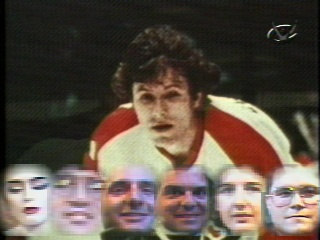
\includegraphics{figures/roar/vtv.jpeg}
	\caption{Screenshot of \emph{Vision Television}, from \citep{vt}}
	\label{fig:vtv}
\end{marginfigure}


\section{Related Work}

In the academic literature, social interaction around television has been a research topic for years. As with the broad interest in CSCW systems work of building systems to support experiences that had historically been co-present, the focus of this research stream has been on recreating the experience of sitting around a television talking about what's on screen. This is the primary goal for essentially all of the systems discussed in this section. 

\begin{marginfigure}
	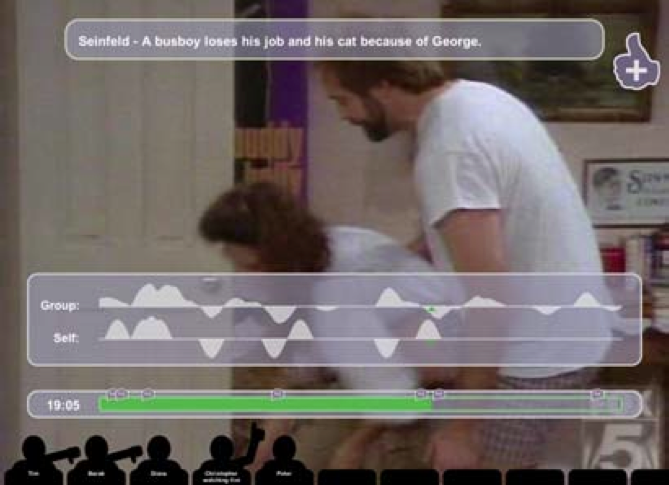
\includegraphics{figures/roar/collaboraTV.png}
	\caption{Screenshot of \emph{CollaboraTV}, from \citep{harrison2007collaboratv}}
	\label{fig:collaboratv}
\end{marginfigure}


There are a number of common threads across all the social TV systems discussed here:

\begin{itemize}
	\item Content is viewed on a television
	\item The system is generalized, i.e. for essentially all kinds of TV content and supports awareness between programs
	\item A buddy-list system provides awareness of others' TV experiences
	\item Co-watching is conceived as an intimate, interactive experience between small groups
	\item There is zero awareness of non-friends \sidenote{This is mostly an artifact of the research context. It's hard enough to arrange a group of 5-10 households in a social network willing to install and use the system, let alone a broader network of unconnected users. Few researchers would bet on the value of crowd interactions when assembling a crowd for experimental purposes is so challenging.}
\end{itemize}




Best practices about how best to handle each of these basic features is discussed by \citep{sociability.heuristics}.
	
Where the systems tend to diverge is how exactly they try to create a sense of co-presence. The main distinction is the primary mode of interaction: symbolic, chat, or voice. In general, researchers agree that voice is a natural and effective way of promoting a sense of co-presence, but that voice has technical and environmental challenges to adoption. Chat can be effective for users who are used to chatting while doing other activities, but for unacclimated users it can be distracting and frustrating. \citep{compare.voice.tex} This finding is mitigated, though, by other researchers who found that when only chat is offered, users report having satisfying experiences. \citep{regan2004media} Symbolic interaction, like a ``thumbs up'' button or pre-canned messages alone are ``simply insufficient and too impersonal for fostering a feeling of connection.'' \citep{examiningpresence} This, too, is countered by  who find that marking ``positive'' and ``negative'' points in a video in an asynchronous viewing context was considered enjoyable. One interpretation of these conflicting findings is that \citet{compare.voice.tex} are less concerned with co-presence because of their interest in asynchronous viewing, so their research focus was not on whether or not people felt like they were watching with their friends, but was instead on simply whether or not they enjoyed marking up video.


\begin{marginfigure}
	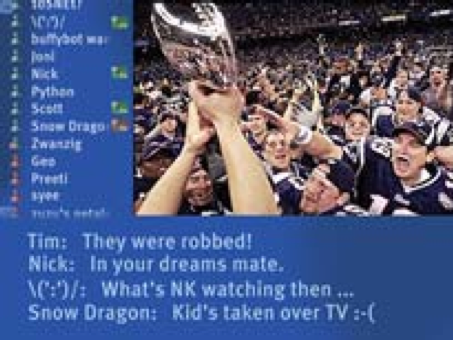
\includegraphics{figures/roar/media_center.png}
	\caption{Screenshot of \emph{Media Center Buddies}, from \citep{regan2004media}}
	\label{fig:media_center}
\end{marginfigure}


Most social TV work responds to the rise of digital video recorders in some way. For systems that are interested in creating a sense of co-presence, the wide-spread availability of devices to both pause shows in real time and record them completely for later viewing poses a major challenge. \emph{CollaboraTV} \citep{harrison2007collaboratv} addresses this most directly, making synchronous and asynchronous viewing essentially identical by providing only a limited vocabulary for interaction to avoid the expectation of actual between-viewer conversation. Other systems that do aspire to supporting synchronous co-present experiences typically make a nod towards potentially time shifting interactions for later viewing by friends.

\begin{marginfigure}
	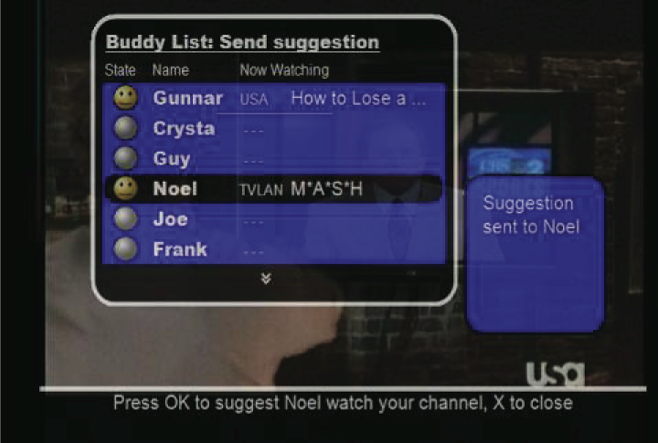
\includegraphics{figures/roar/socialTV.png}
	\caption{Screenshot of \emph{SocialTV}, from \citep{uses.socialTV}}
	\label{fig:socialTV}
\end{marginfigure}


The final major axis of distinction is around the representation of viewers. \emph{Social TV}\citep{harboe2007perceptions}, \emph{Media Center Buddies}\citep{regan2004media}, \emph{2BeOn}\citep{abreu20022beon}, and \emph{ConnecTV} \citep{boertjes2008connectv} all use buddy-list metaphors throughout the experience. Other systems like \emph{AmigoTV} \citep{coppens2004amigotv}, \emph{CollaboraTV} \citep{harrison2007collaboratv}, and \emph{Vision Television}\citep{vt} focus on using either real or iconic versions of faces to represent viewers. Most of these support ways of animating those avatars in ways that indicate an emotional state in response to the program.

\begin{marginfigure}
	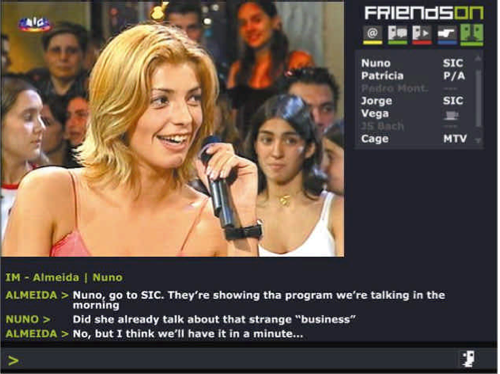
\includegraphics{figures/roar/2BeOn.png}
	\caption{Screenshot of \emph{2BeOn}, from \citep{abreu20022beon}}
	\label{fig:2beon}
\end{marginfigure}


\emph{ROAR} sets itself apart from this past work in a number of ways. Due to technical constraints in the period when this work was most popular, almost all social TV systems used the TV screen as site of the user interface.\sidenote{The one notable exception is \citeapos{Fink:2006td} work, which also shares an interest in creating ``ad-hoc'' groups in a broadly-similar way that \emph{ROAR} constructs sections.} \emph{ROAR}'s focus on supporting interactions around video watched on a computer is a marked difference in approach that has a number of benefits: text input is easier, the interface can have finer details because of increased resolution and shorter viewing distances and multi-user scenarios are quite rare. This was, of course, an approach that was historically possible, but the recent availability of wide-spread access to streamed versions of live events has made this venue more viable. Furthermore, consensus seems to have emerged that interaction in a traditional TV context is going to be tablet and mobile phone centric, not taking place on the TV screen itself.

\begin{marginfigure}
	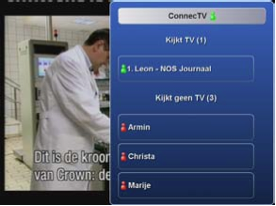
\includegraphics{figures/roar/connectv.png}
	\caption{Screenshot of \emph{ConnecTV}, from \citep{boertjes2008connectv}}
	\label{fig:connectv}
\end{marginfigure}



The other most important difference between \emph{ROAR} and past social TV work is its interest in supporting awareness among all viewers, not just between viewers with a pre-existing relationship. There is some work in this space, like \emph{Visual Backchannel}\citep{Dork:2010fb} that focuses on providing reflective tools for analyzing and browsing through tweets with a particular hashtag. But there is little work in trying to build interfaces that merge participation with real-time shared visualization. The co-incidence of participation and visualization is a critical component to grounding, as discussed throughout this thesis. If the visualizations of group participation are not part of everyone's shared display, they lose value as a site for collective action - one of the main goals of \emph{ROAR}'s crowd visualizations.

\begin{marginfigure}
	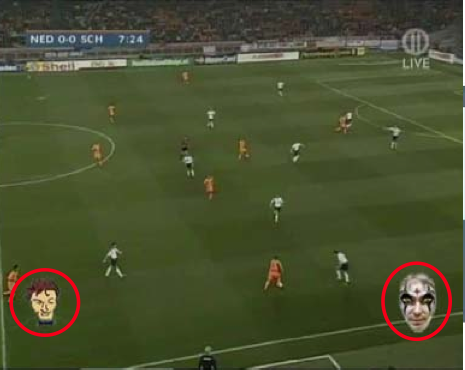
\includegraphics{figures/roar/amigotv.png}
	\caption{Screenshot of \emph{AmigoTV}, from \citep{coppens2004amigotv}}
	\label{fig:amigotv}
\end{marginfigure}

Although \emph{ROAR} is interested in co-presence, it aims to live in somewhat more ambiguous social settings where groups are made up not necessarily just of close friends (where voice might be comfortable) but with somewhat larger groups where 5-10 people might co-watch with different levels of engagement. Although voice is a richer experience, it has relatively hard limits in terms of numbers of active participants. Furthermore, voice tends to be a higher intimacy channel, which is less useful in contexts where not everyone necessarily knows everyone else. Thus to support co-presence, \emph{ROAR} focuses on chat and some other associated features like polls and drawing. This focus on co-presence precludes creating in any serious way an asynchronous version of \emph{ROAR}. Indeed, \citet{uses.socialTV} note that among some mixed results, the strongest experiences were in live events like sports. 




% Motorola SocialTV work: underlines the need for free form messaging. ``lightweight messages alone were simply insufficient and too impersonal for fostering a feeling of connection''
% 	features: buddy list, offline presence through ambient devices / chumby. invite to show, and simple symbolic messaging and pre-canned messages. \citep{examiningpresence}
% 	
% 	
% review paper: series of general guidelines. weirdly prescriptive about what social tv is, but whatever. 
% 
% 
% \citep{uses.socialTV} is a sort of depressing ``nothing works'' piece. notes that it's particularly good for sports
% 
% fink et al 2006 provides chat on a computer 
% 
% 
% \citep{harrison2007collaboratv} has a nice system with an MST3K style silhouette at the bottom with thumbs up / down. compared it (sort of) to a chat system, with people preferring the avatar system
% 
% amigoTV \citep{coppens2004amigotv} heavily avatar-based , using avatar animation to communicate (plus all the usual presence notification work) voice and some text chat
% 
% \citep{regan2004media} text based, on screen. built into MSN. found people liked the chat experience 
% 
% \citep{abreu20022beon} another on-tv one with chat. basic outlines similar to roar - chat along bottom, something else on the right side. no eval.



% A Visual Backchannel for Large-Scale Events
% get andrea's bibliography and pull from there





\subsection{Other Conversational Tools}

Social TV research has faded somewhat in popularity since the mid 2000's.  There is a widely-held assumption that conversations around live events are going on not in TV-specific interfaces like those built by researchers, but instead on existing social networks like \emph{Facebook} and \emph{Twitter}. In this model, when someone wishes to interact with friends or strangers watching the same event as them, they simply turn to existing social network channels. If this were true, it would suggest that \emph{ROAR}'s approach is deeply flawed, and instead our focus should be on building systems that use \emph{Facebook} or \emph{Twitter} as a substrate. This approach would look much more like \emph{Visual Backchannel}\citep{Dork:2010fb}. However, I will argue in this section that the social spaces created by \emph{Facebook} and \emph{Twitter} are not (and barring fundamental changes to their mechanics can not become) spaces for truly interactive discussions about a live event. Instead, we need a new platform to be the home for these conversations.

As I've argued about grounding elsewhere in this thesis, creating social situations with mutual awareness is critical to creating effective conversation spaces. If there is any concern that others can't see what you're saying, it breaks the cycle of awareness that is critical for moving a conversation forward. The publish/subscribe model adopted by and \emph{Twitter} gets in the way of this once conversations scale beyond just one person. If Bob follows Alice, and Charlie follows Alice but not Bob, Charlie will see only parts of a conversation that are not directed at Bob with an ``@'' reply. \sidenote{I'm going to mostly ignore \emph{Facebook} for the sake of simplifying the argument. The outlines of the argument are similar, but \emph{Facebook}'s more integrated reply format avoids some of these problems. This is offset by the lack of reliability of posts being seen by friends; as few as 20\% of your friends see any given post \citep{Constantine:2012uk}.}

The nominal solution for this is hashtags, e.g. words prefixed with a ``\#'' character. These mark a tweet as part of a larger set of tweets on a theme, and places that tweet in a stream in the so-called ``discover'' part of the interface. This interface has a similar grounding-inhibiting design. First, it is impossible to tell if others are actively viewing the hashtag in the ``discover'' mode. Whether or not that audience exists is essentially unknowable to posters. Hashtags are visible amongst follower networks (i.e. you can see hashtags that seem to be popular within your network and be involved in this conversations) but there is little evidence that participations cross existing follower/following relationships.

The problem of an audience for tweets with a hashtag is compounded because tweets with a hashtag do have one guaranteed audience: your existing followers. Every tweet, hashtagged or not, is inserted in the streams of all your followers. When balancing a potential imagined audience and a guaranteed one, people will write for the audience they know they have. For major events like the Superbowl or World Cup, we can safely assume that our audience is likely to contain many people who are watching the same event. But even for moderately less popular events, it is far more likely that most of our followers are not co-watching and are unlikely to be deeply interested in a detailed conversation about what's happening. 

We can see that this is true by looking at the sorts of tweets that people write during live events like conferences. \citet{Ebner:2010tx} try to categorize conference tweets into four categories: irrelevant tweets, administrative tweets, topical discussions, and topical tweets. The distinction between the latter two categories seems to be whether a tweet contains an ``@'' reply or not. The authors argue that without external information like a link or picture, a tweet is too decontextualized to be valuable to a non-attendee. I see their data differently. If we look at their exemplar topical tweets (excluding questions, whose audience is clearly the presenter), most of them are clearly written for an audience that does \emph{not} share their context.  For example, the tweet ``nice idea of @estudyskills Aggregation of all student weblogs at Tumblelog - gives overview. \#ec10hh'' is recording the content of a talk for someone who isn't there. A simple evaluation-oriented tweet like this for a co-present audience would look a lot more like ``nice idea of @estudyskills'' and leave off the rest of the context. Indeed, this is the core difference between chat messages and posts to \emph{Twitter} or \emph{Facebook}: chat messages rarely make sense out of context, but posts are nearly always written with context included to make them comprehensible to a non-present audience. 

% do an informal analysis of tweets for the latest ML talks event. categorize into announcements, quotes, other https://twitter.com/#!/search/realtime/mltalks

While looking at how people write tweets versus chat messages is interesting, volume of participation is also interesting. We can look at summary data from Bluefin Labs, a company that captures and analyzes \emph{Twitter} conversations about TV shows and compare the participation rates in \emph{Twitter} conversations to similar chat conversations. For each show they analyze, they report the total number of tweets about the show and the total number of people who tweeted about the show. The ratio of these two values is the average number of tweets per tweeter. For the vast majority of shows they track, this value is between $1$ and $2$; the average viewer tweets at most twice about a single show. This holds true even for sports matches that can last 2-3 hours. It is intuitive that only one or two messages per person is a strong indication that there is not significant conversation going on; conversations simply cannot take place in one or two messages. Nevertheless, it is useful to compare these participation patterns with a social context that looks more like \emph{ROAR} to argue for \emph{ROAR}'s design approach.

% put in a screenshot of the blue fin data page

Although we don't have data for people using a system like \emph{ROAR} yet, we can look to comparable experiences that already exist. Many sports fans use platforms like Internet Relay Chat to talk about live events. Based on logs collected over the course of two weeks, we can calculate a metric similar to that reported by Bluefin Labs for conversations on \emph{Twitter}. We can't easily link specific messages to specific events, but we can measure how many messages each person sends per hour in which they send any messages at all; essentially for people who are chatting in a given window, how many messages do they send? This approximates the tweets per unique author per show metric. This measure varies pretty substantially between which chat room you collect data from. Data is reported in Table \ref{tab:chat_message_rates}. 


% channel name
% average unique hourly users (average )
% total messages  \sigma{msg}
% total duration t_n - t_0
% average messages per active user
% comments

\begin{table*}[tb]
\begin{tabular}{r|lllll}
\textbf{Channel} & \textbf{Total Messages} & \textbf{Total Users} & \textbf{Mean Hourly Active Users} & \textbf{Mean  Messages Per Active User-Hour} \\

\#reddit-soccer & 20,317 & 251 & 7.9 (SD=9.9) & 16.6 (SD=25.5) \\
\#football & 11,936 & 199 & 8.8 (SD=8.2) & 10.1 (SD=11.8) \\
\#teamliquid & 110,910 & 1,940 & 29.7 (SD=19.2) & 9.5 (SD=18.1) \\
\#joindota & 93,010 & 9,022 & 52.8 (SD=113.3) & 3.4 (SD=9.6) \\
	
\end{tabular}
\label{tab:chat_message_rates}
\caption{Comparison of participation rates across different IRC chat rooms.}
\end{table*}

The most direct comparison to \emph{Twitter} is the final numeric column on the right. Mean messages per active user-hour represents the average number of chat message a user sends in hours where they send any messages at all. If every user logged on, sent one message, and then stayed silent, this metric would be 1. It would also be 1 if every user sent one message per hour. As a result, the floor of this metric (as with the tweets / unique author metric) is 1. Larger values represent users who tends to send many more messages during hours where they are chatting at all. This metric is artificially depressed relative to the \emph{Twitter} metric because our data covers not just moments when there are live events going on, but 24 hours a day. This is captured by the variance in the fifth column: the number of active chatters varies widely between active moments and inactive moments. Inactive moments don't exist in the \emph{Twitter} dataset because it focuses on only the tweets associated with a television show. Despite this, we see values ranging from 3.4 to 16.6, compared to \emph{Twitter}'s 1-2. This suggests that chat contexts elicit a 200-1600\% increase in per-active-user participation. 

The large variance in participation rates seems (in this very preliminary review) to be correlated with the size of the rooms. The rooms with the highest per-user participation were also the rooms with the fewest active users. This supports the \emph{ROAR}'s core argument that smaller interaction contexts will be more interactive than larger undifferentiated contexts. This might also explain part of the difference between \emph{Twitter} and a chat-style system: \emph{Twitter} looks much more like a single large undifferentiated room than a focused small scale social space.

This informal analysis underlines both the strong differences in behavior in post/subscribe models like \emph{Twitter} or \emph{Facebook} compared to chat-based designs like \emph{ROAR}.




% We can see th

%The easiest way to understand that is does is exist would be getting a reply from someone who doesn't follow you who discovered your tweet via the ``discover'' tab. Although this is possible, a casual perusal of tweets involved in trending topics shows vanishingly few replies to other tweets; RTs are far more common. These impediments to mutual visibility 

% would be interesting to make an empirical argument about how many @ replies are to people via hash tags. could try to do this by looking at @ that were replied to that were between people who don't follow each other and have used a hash tag in a period. that's a bit elaborate, though. 

% make a diagram of the alice/bob/charlie system
% put a screenshot of the discover interface in here in



\section{Design}

\emph{ROAR} is a social platform that wraps streaming video of a live event. This section will cover the basic components of a web-based version of \emph{ROAR}. An overview of the visual layout is shown in Figure \ref{fig:roar_overview}. 

\begin{figure*}
	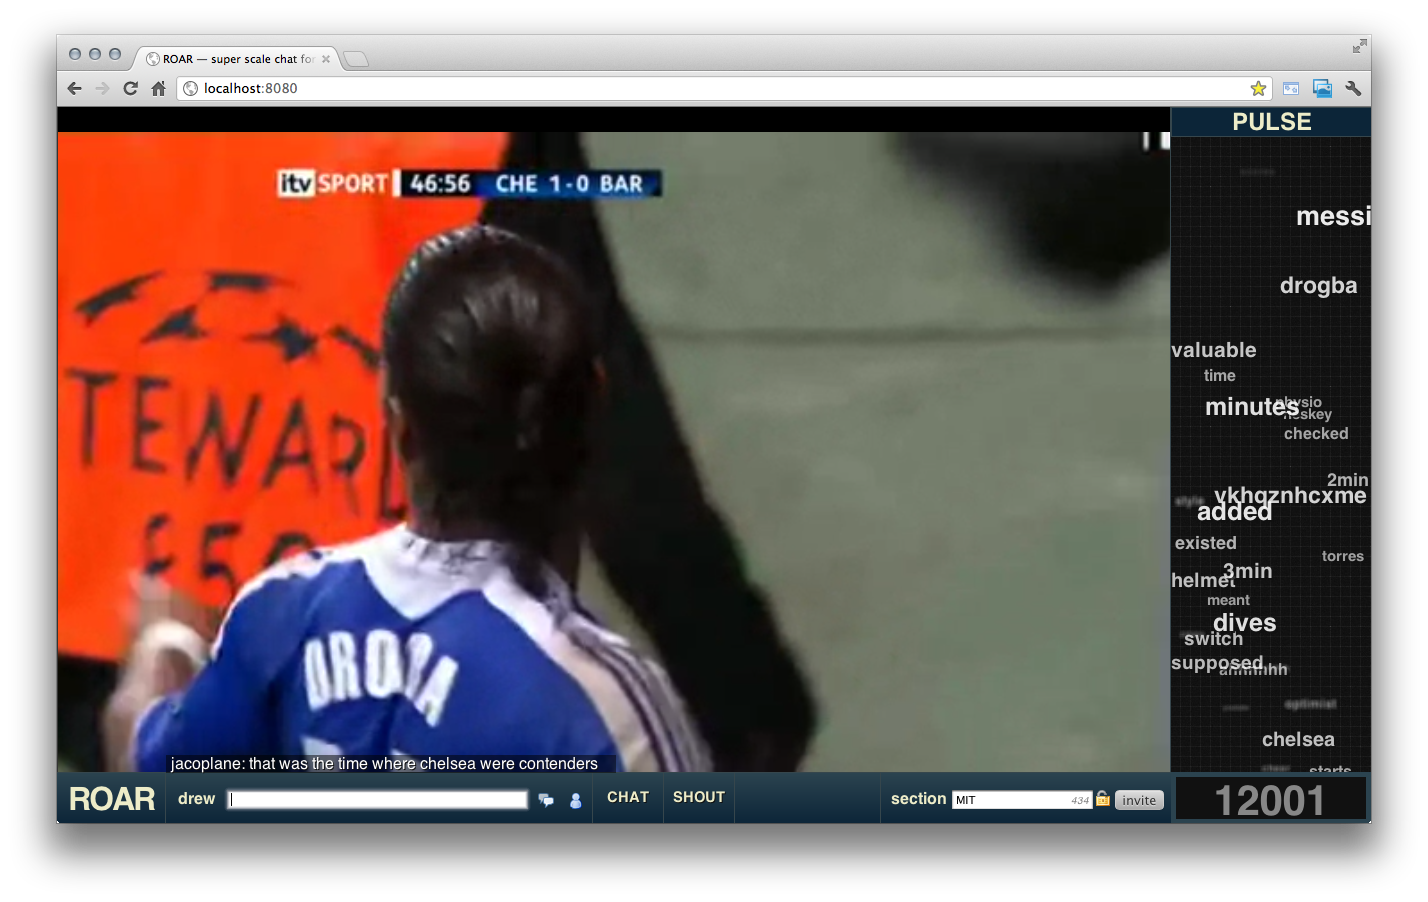
\includegraphics{figures/roar/overview.png}
	\caption{An overview of the \emph{ROAR} interface.}
	\label{fig:roar_overview}
\end{figure*}


\subsection{Sections}

I take the organizing metaphor of a ``section'' from the physical experience of being in a crowd at, for instance, a sporting arena. Audience members rarely come to a stadium alone: most people come with friends. Existing tools for watching live events with chat tend to simply group all viewers into one anonymous mass. As I argued in the previous section, this approach tends to depress overall participation because too much chat can crowd out deeper and broader conversations. In contrast, \emph{ROAR} organizes viewers into many  smaller sections. Each section can be named or unnamed. 

When a viewer joins a \emph{ROAR}-enabled stream, they are provided with a section browser. If they log in with a \emph{Facebook} or \emph{Twitter} account, \emph{ROAR} can prioritize sections with friends in them. A draft of this interface is shown in Figure \ref{fig:roar_section_browser}. For viewers who don't want to log in with \emph{Facebook} or \emph{Twitter}, they can search for named rooms on a particular theme, like a school, employer, location, or team they're a fan of. Conceptually, sections are like tables at a bar or circles of people at a cocktail party. You're likely to know at least some of the people at a table you want to join, but not necessarily everyone. It's easy to scan the room to evaluate options. When you're in a section, most of your attention is focused on the interaction within that section, but there are a number of other systems that try to maintain some awareness of the crowd as a whole. 

\begin{marginfigure}
	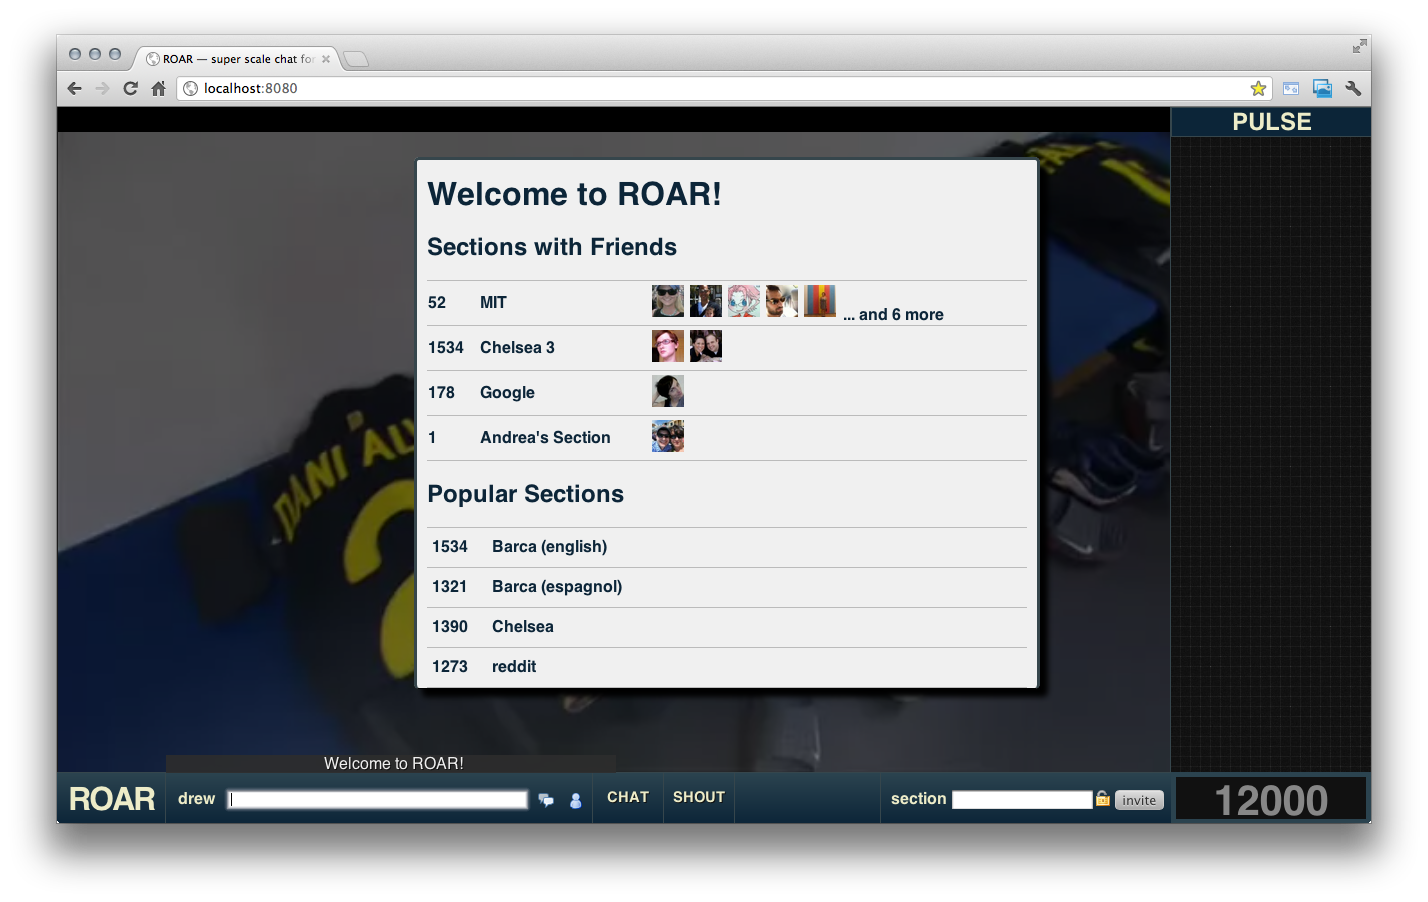
\includegraphics{figures/roar/roar_sections.png}
	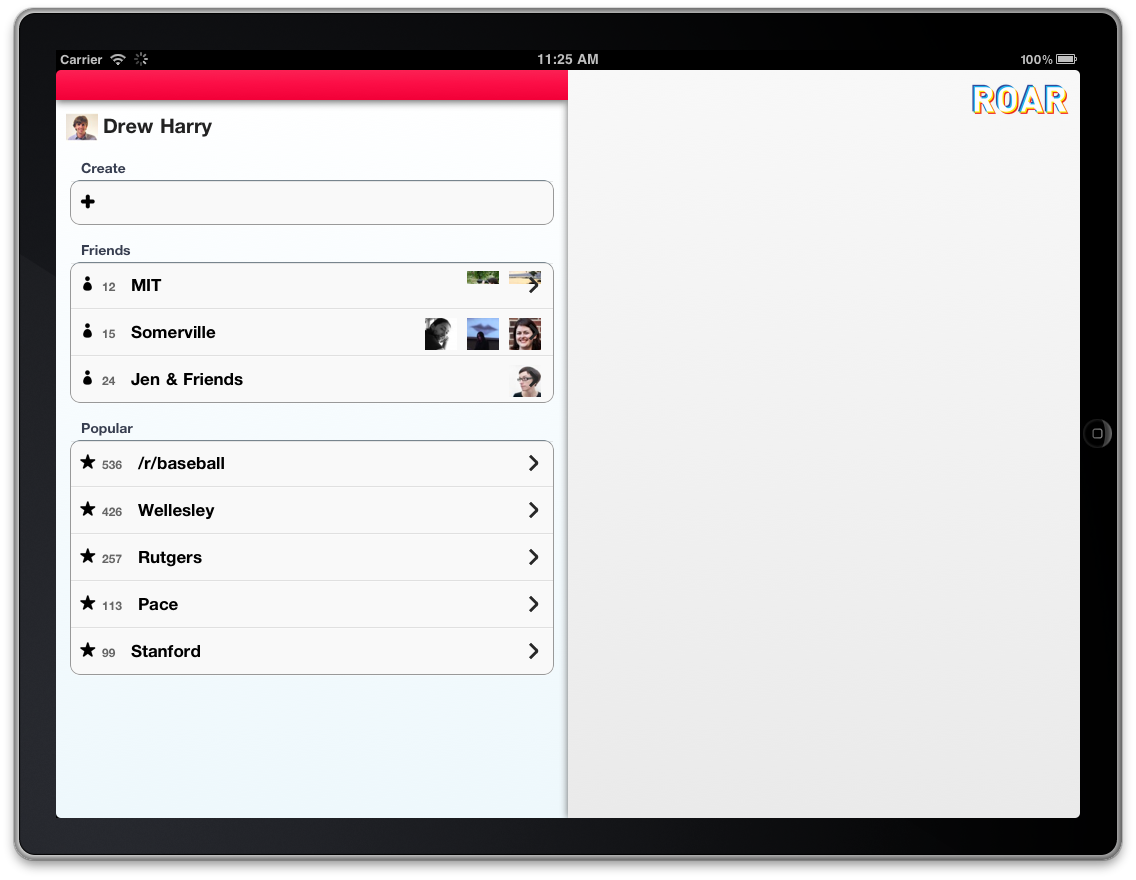
\includegraphics{figures/roar/roar_sections_tablet.png}
	\caption{View of the section selection interface on a web interface (top) and tablet interface (bottom).}
	\label{fig:roar_section_browser}
\end{marginfigure}

There are a variety of potential interaction styles within a section. Chat is the dominant one shown in this prototype, but chat depends on easy access to a keyboard. It is easy to imagine versions of \emph{ROAR} that would make sense on a mobile phone or tablet device. In these contexts, text entry is somewhat more challenging, so having interaction models that require less text entry but that still support a sense of presence would be valuable.

There are two varieties of interaction that the \emph{ROAR} prototype supports. The first is the ``shout.'' Shouts are composed less like chat messages, and more like tweets. They are intended to be shared out of context to more people. A shout might be a witty comment, a link to a funny image about the game, a clever insult to a hated player or team, or simply a message that captures the feeling of the crowd at that moment. When a shout is entered, it is shown first to viewers in the section of the author. Unlike chat messages, shouts can be voted for. Shouts that accumulate enough votes within their initial section will spread to other sections. \sidenote{There are a number of moderation challenges with shouts that will be addressed later. Shouts are also significantly rate-limited, and having previous shouts judged negatively by a moderator will strongly increase this rate-limit.} Eventually, widely popular shouts could spread to the entire audience, while some will peter out having only been seen by a small fraction of the crowd as a whole.

The second variety of novel interaction is the creation of graphical signs. Although this doesn't make much sense with a traditional keyboard and mouse interface, drawing is much more natural on tablet devices. For users in that context, drawing can be more expressive than typing. The creation of signs meshes nicely with existing fan practices around bringing signs to a stadium. Indeed, signs brought to the stadium are explicitly written to attract the attention of camera-operators and commentators with the hope of being broadcast to the remote audience and put on a live display within the stadium. In this way, the practice of sign creation is already implicitly acknowledging the attention and awareness of the remote audience. Empowering remote fans to participate in this practice seems like a natural extension, especially on input devices where drawing is easy and accessible. An example of the drawing interface and a sign's representation in the section stream are shown in Figures \ref{fig:roar_sign}.

\begin{marginfigure}
	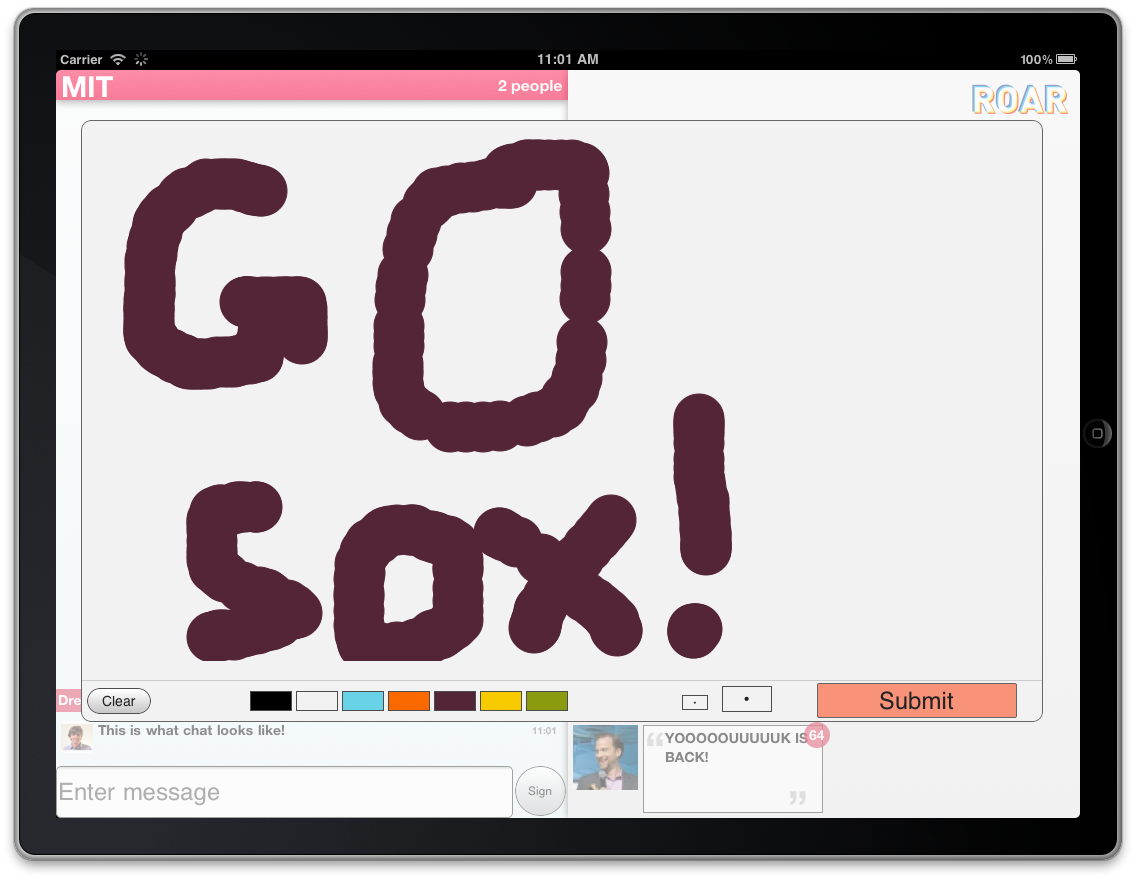
\includegraphics{figures/roar/drawing_sign}
	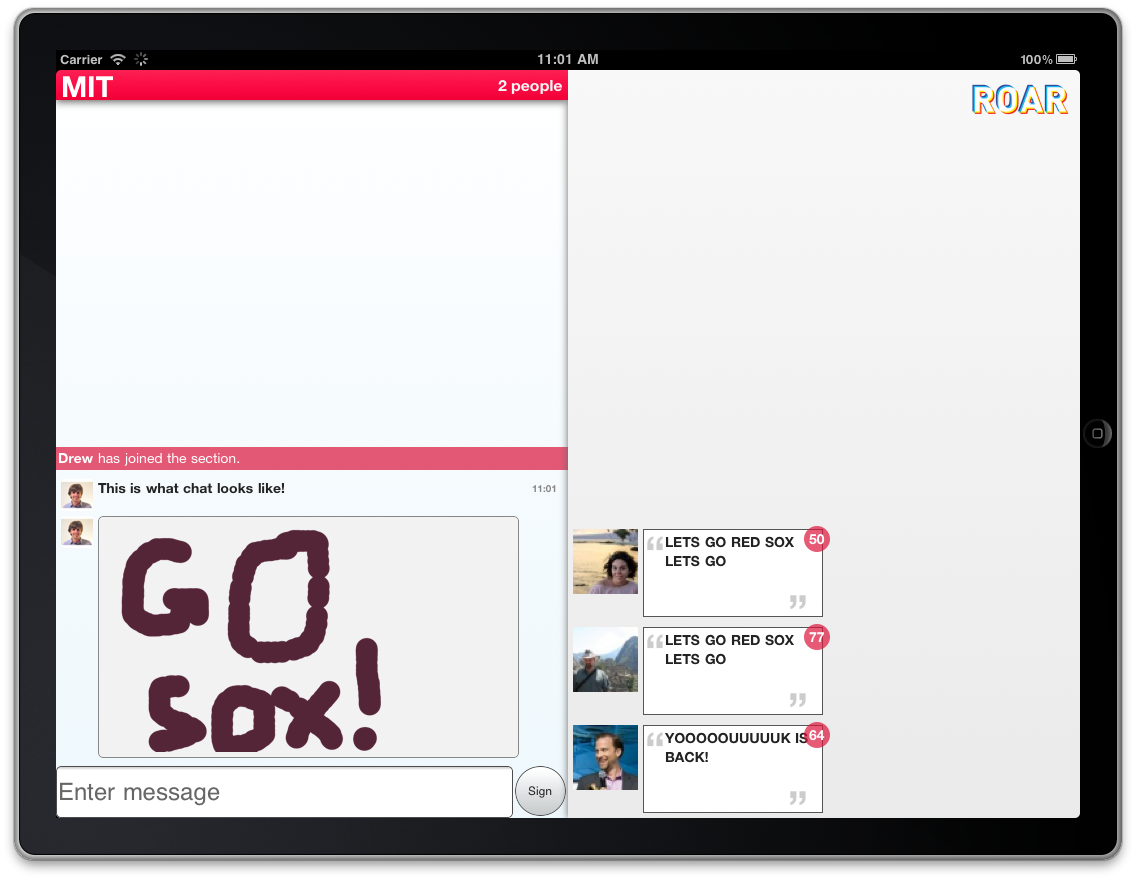
\includegraphics{figures/roar/sign_in_section_chat.png}
	\caption{Top, an interface for drawing a sign in a tablet interface. Bottom, that sign displayed in a section stream.}
	\label{fig:roar_sign}
\end{marginfigure}

% talk about question-asking ala backchannl? probably not.

As a primary communication medium, non-audio communication has a number of major advantages for \emph{ROAR}. Chat requires minimal extra hardware, can be done in loud places, is more easily analyzable at large scales, doesn't require turn-taking, and requires substantially less technical infrastructure to support at scale. Still, it is far less immersive and communicative than voice communication. Although audio becomes problematic for large groups (for reasons discussed throughout this thesis), the potentially small size of sections might mean that for groups of 3-5 audio could be an effective addition.

% TODO talk about section categorization and recommendation? 


\subsection{Predictions, Betting, and Promoting}

Although chat is the foundation of creating a sense of presence with other people in a section, this thesis has argued throughout for the value of non-verbal actions that provide lighter-weight senses of presence. These kinds of actions can help remind section-members of the presence and engagement of people who might not have something to say, but are still attending to the section and the event. In the context of \emph{ROAR} there are a number of different kinds of non-verbal actions that would be appropriate.

The most simple of these actions is making predictions. An event organizer could pose a question to an audience like ``Which team will win the game?'' These questions could be section-specific or global. Responses to a prompt like this can be aggregated globally or (more importantly) be represented within the section to catalyze a discussion. A simple version of this is shown in Figure \ref{fig:roar_voting}. These questions could also come from section-members and be scoped just to the section.

\begin{marginfigure}
	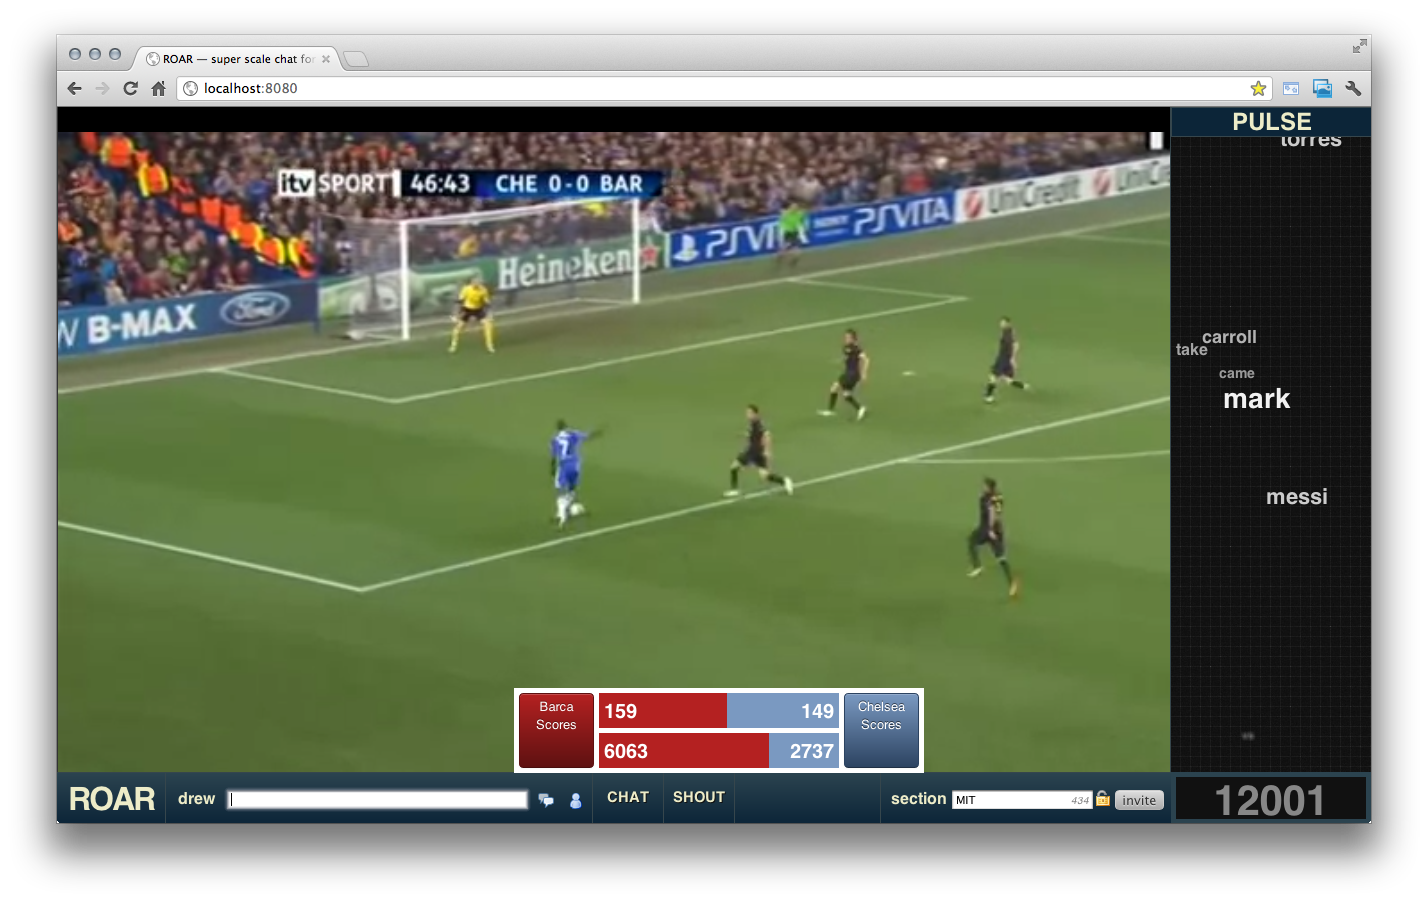
\includegraphics{figures/roar/voting.png}
	\caption{In the bottom center of the screen, an open vote. The top bar is votes within your section, the bottom bar is global votes.}
	\label{fig:roar_voting}
\end{marginfigure}

These sorts of lightweight predictions make sense across a wide range of the sorts of events that \emph{ROAR} aims to support. Live competitive performance shows like \emph{American Idol} or \emph{The Voice} have occasional moments where the audience could weigh in and change the course of the show. Sports-oriented events could offer an even more elaborate and high-frequency interaction. Instead of the occasional audience-wide poll, fans could place time-sensitive bets on the outcomes of various game events. Baseball provides a particularly effective example. Within a single game, there are a series of interlocking time scales where predictions make sense from the inning to the individual batter, to the individual play. At each of these levels, a viewer could opt to place a bet about the outcome of the event. These bets would be shared at the section level, and effective betters would be highlighted on a leader-board. While these kinds of actions don't make sense for all events, they're another design element that could be added or subtracted depending on the style of event. 

All sorts of section and crowd-level participation can also support voting to guide the promotion of interesting content and the identification of inappropriate content. This serves as an additional stream of non-verbal actions for the engaged but perhaps not verbally inclined viewer. Votes are aggregated for shouts and signs, and used to spread those contributions to a wider audience. This serves to create a stronger relationship within the audience. By participating in identifying the sorts of content you like, it creates a sense of the community's values represented in the top contributions as judged by viewers. It also supports a sense of ownership. Without voting, the acknowledgement of a crowd contribution on-air (in the way that cable news now frequently takes tweets out of context and discusses them on-camera) seems arbitrary and analogous to shouting requests to a band during the breaks between songs. Whether a message catches the attention of the performer or anchor is essentially arbitrary. But by being able to identify contributions that you see as valuable, you can buy into the success and quality of that contribution and celebrate its broader spread rather than rue the arbitrariness of a random selection process.

One of the major benefits of nonverbal actions like those discussed in this section is their ease of aggregation. As in \emph{backchan.nl}, where voting serves as a simple low-impact way to participate which guides the system's decisions about what content to show on the main screen, non-verbal actions like making predictions, placing bets, or voting for other kinds of content can be easily aggregated across all sections and represented back to the crowd as a whole. This create a continued reminder of the crowd's presence in the same space. Furthermore, \emph{ROAR} could leverage the existing infrastructure in the physical spaces where events take place to represent the remote audience back to the co-located audience. Using the example of audience-drawn signs, we can imagine using jumbotron in a stadium, for instance, as a venue to share remote audience content that has been voted up. This creates a strong incentive for creating and voting for content because, as in \emph{backchan.nl}, the shared screen carries with it a guaranteed audience for your contribution. Having something you created or promoted appear in the main video stream in a physical space closes the feedback loop, and reminds physical spectators and remote spectators of each others' presence. An example of this approach is shown in Figure \ref{fig:roar_fenway_sign}. As with using shared displays in other projects in this thesis, using existing displays in physical venues can help ground the experience between remote and local audiences and create a stronger sense that they are sharing an experience.

\begin{marginfigure}
	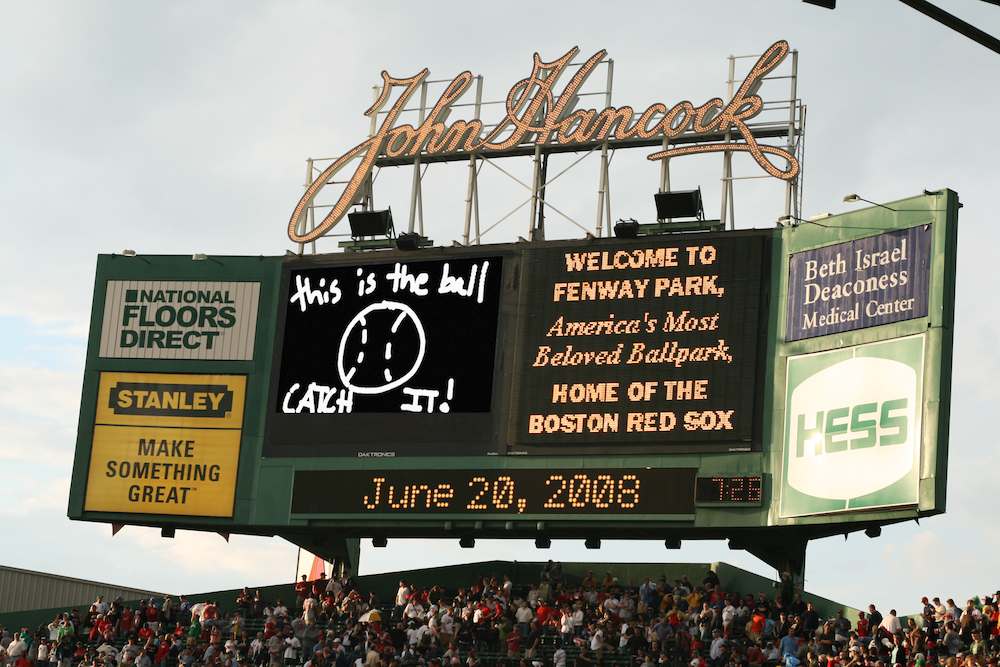
\includegraphics{figures/roar/stadium_sign_small.png}
	\caption{A sign drawn by an audience member displayed on screen in the stadium.}
	\label{fig:roar_fenway_sign}
\end{marginfigure}


\subsection{Pulse}

Section-oriented features focus on creating a small scale sense of community between small groups of viewers. While this is part of an enjoyable spectating experience, an awareness of the crowd as a whole is a critical component to the \emph{ROAR} vision. More than any other feature in \emph{ROAR}, the crowd visualization has evolved considerably over the design process. In this section, I will describe each of these designs, and explore the extent to which they satisfied the different sorts of awarenesses you can have of a physical crowd:

\begin{description}
\item [Volume]{How active is the crowd right now, relative to the recent past?}
\item [Topics]{What topics is the crowd talking about right now, and what are they saying about those topics?}
\item [Collective Action]{More speculatively, might we be able to give the crowd opportunities to do some sort of activity analogous to singing or chanting?}
\end{description}

Each of the designs described here is supported by a keyword detection algorithm that is essentially unchanged across the visualizations. The algorithm scans all chat messages and applies an adapted version of the Term Frequency, Inverse Document Frequency algorithm to identify words that are globally uncommon but frequent in the last few seconds of chat. TF-IDF depends on a notion of documents, and compares the term frequency within a given document to all other documents within the corpus. For a real time stream of data like chat, this obviously requires some adaptation. \emph{ROAR} bins all chat into 10 second windows of chat, and treats those as documents as far as TF-IDF is concerned. This makes sense conceptually because we can assume that chat is about the video, and as the contents of the video shifts over time, the conversation about it will as well. This means we can reasonably assume that each window of chat will function similar to documents in a traditional TF-IDF model. Of course, this assumption is not iron-clad, and can lead to quite noisy results. All the chat shown in screenshots of these visualizations is recorded from Internet Relay Chat rooms organized to discuss various spectator events like video game tournaments or sports matches. 

The analysis engine provides a rank-ordered list on a per-window basis (10s) of the words with the highest recent TF-IDF scores. I call this list the ``term rankings.'' \sidenote{The size of this window is purely a function of chat rate. At high chat rates, this window can shrink substantially and decrease the latency between a new term appearing and it being recognized by the algorithm. At low chat rates, the window needs to grow larger so build larger enough bins to do a reasonable analysis.} This is the input to each of the visualizations described here. It is quite common for subsequent rank ordered lists top words in the last analysis window to share very few words with any previous analysis window. This high amount of turnover poses a design challenge that each design deals with in different ways: how much inertia should be added to the visualization to dampen out the inherent noisiness of the term rankings? 


\begin{figure*}[tb]
	\includegraphics{figures/roar/cloud.png}
	\caption{A word-cloud style visualization where words appear when first seen in a term ranking list and fade over time.}
	\label{fig:pulse_word_cloud}
\end{figure*}

% initial word cloud on top of video

The first visualization adopted a word cloud model. When a word appeared in the term rankings list, that word was added to the word cloud. The higher its position in the term rankings, the larger the initial size of the word. Each second, every word currently displayed in the visualization would decay in size slightly. If a word already displayed in the cloud appeared in a subsequent term ranking list, its size would be increased, correlated with its ranking in the list. If a word slipped below a certain size, it would fade out of the cloud. The cloud was rendered on top of the live video, ostensibly in a part of the screen that was not as critical to viewers. This approach is shown in Figure \ref{fig:pulse_word_cloud}

This visualization had a number of valuable properties in terms of our three original goals. Volume and topics were both easily comprehensible in this format. In particular, the spatial stability of words (i.e. they stay in more or less the same place on the screen for their lifetime) made it easy to both track the performance over time of an individual topic and not be distracted over-much by constant movement. This approach struggled with the temporal component to the data, though. It combines terms that were historically popular but haven't yet decayed enough to be removed with up and coming words. While the lack of a time component simplifies the visualization, it also makes it somewhat less effective for collective actions like cheering or chanting because earlier stages of a cheer are conflated with current ones. Perhaps the biggest problem with this approach is its space inefficiency. Responding to a demo video using this visualization style\sidenote{This visualization can be seen in motion in this demo video: \url{http://www.youtube.com/watch?v=KK13_jE_NGg}}, potential users expressed an intense dislike for any approach that attempted to overlay the video itself. As a result, all future visualizations are located at the edges of the screen using pixels dedicated for visualization, not attempting to overlay the video.

\begin{figure*}[tb]
	\includegraphics{figures/roar/bar.png}
	\caption{A direct visualization of the term rankings. Larger words have higher rankings, and the total number of words is correlated to the volume rating at that moment. This list changes completely on each new term ranking list.}
	\label{fig:pulse_rankings}
\end{figure*}

The other major drawback of the word cloud approach is the lack of semantics to the position of words. The next three visualizations use screen location in a variety of ways. The most direct approach was to simply display the term rankings along the bottom of the screen underneath the main interface bar, shown in Figure \ref{fig:pulse_rankings}. In high activity periods, words lower down the term rankings were shown. In this way, the total number of words displayed functioned a bit like a volume meter, and the most important words always occupied the same part of the screen. However, the noisiness of the underlying data made updates distracting. A word could easily jump from the top spot to the bottom of the list between subsequent updates, which made it hard to track the life cycle of a term you were tracking. 

Using the same part of the screen, our next approach adopted a river metaphor in which terms would appear on the left edge of the screen when they first appeared in the term rankings and move smoothly to the right. This better introduced a sense of time that was missing from earlier approaches. If words continued to appear in the term rankings, they would grow in size. If they were missing from the term rankings for a few cycles they would fade away completely. This ensured that any word still showing had appeared in term rankings at least once in the last 10 seconds. Furthermore, words that made it all the way to the right edge had at least been present in the term rankings for a while, making the right side of the visualization a reliable space to see long-term popular words. This approach is shown in Figure \ref{fig:pulse_river}.

\begin{figure*}[tb]
	\includegraphics{figures/roar/river.png}
	\caption{In this visualization, words appear on the left edge as they appear in term rankings and move smoothly to the right. Larger words move more slowly than smaller words.}
	\label{fig:pulse_river}
\end{figure*}

\begin{marginfigure}
	\includegraphics{figures/roar/bubble.png}
	\caption{Similar to the river-style visualization, in this approach words appear at the bottom and rise smoothly to the top. In this screenshot, there is relatively low activity.}
	\label{fig:pulse_bubble}
\end{marginfigure}

While this did create a nice sense of a time passing, there are a number of challenges to this approach. In order to handle a high word density in a tight space, it proved necessary to vary the velocity of each word slightly so they never permanently overlap in a way that makes them illegible. This subtly breaks the contract implied by the spatial configuration; no longer is a word's horizontal position tightly correlated with the age of the term. Furthermore, it seemed sensible for words higher on the term ranking list to be larger, and to maintain a physical metaphor it seemed like larger objects should move more slowly and be on screen longer than small objects. Ultimately, this seemed to be enough at odds with the underlying metaphor that time moves left to right and an object's position on the timeline should represent its age. In a tight visual space, it was too difficult to both satisfy that constraint, make it readable, and manipulate the visibility of words in ways that would properly highlight the highest performing words.

The final design iteration took the basic mechanics from the the horizontal, river-like visualization and mapped it onto the vertical axis. Even with the same basic visualization mechanics, words rising up from the bottom instead of moving left to right helped alleviate the sense that position was mapped tightly onto time. Instead of a river, there is a stronger sense of bubbles rising. To reinforce this sense, a simple visualization of the crowd size could be added in the lower right hand corner, from which the words would appear to be rising. The shifted location within the interface also makes it easier to provide an interactive component. In this version, clicking on a word causes a dialog box to slide into place showing the chat messages that triggered that word's inclusion in the visualization. This provide a convenient way to shift from very high level abstractions on the word level down to individual messages. It might also serve as a way to navigate between sections to spaces where there seem to be interesting conversations happening. This final approach is shown in Figure \ref{fig:pulse_bubble} and Figure \ref{fig:pulse_bubble_detail}.\sidenote{A video version of this approach can be found here: \url{http://www.youtube.com/watch?v=Ky9U1v38zsk}}



Returning back to the original values for this visualization, the final visualization approach meets all three goals in an acceptable (if not totally perfect) way. Volume is represented by the bursts of new words at the base of the visualization. This helps show instantaneous increases in participation. Furthermore, it has essentially the same property as the word-cloud approach where the total number of words on screen is loosely correlated with an average of recent activity. In this version, truly popular and long-lasting topics are better distinguished from transient topics, and new topics and easier to differentiate from popular old topics because of the way the words move through the visualization space. This also better supports the sorts of collective action concepts we have in mind; the words of a chant could appear out of the bottom one at a time and not be confused with prior words in the sequence. The biggest remaining weakness of this visualization is that its heavy reliance on motion could be distracting from the primary event content. To help alleviate this, the visualization could be easily run in a minimized mode where only one or two words at a time are shown and travel very slowly so as not to take away from the action during tense moments.

\begin{marginfigure}
	\includegraphics{figures/roar/bubble_detail.png}
	\caption{A view of the bubble-style visualization during a high activity period. Clicking on a term brings up a view of messages that led to that term's appearance in the term ranking list.}
	\label{fig:pulse_bubble_detail}
\end{marginfigure}


\subsection{Moderation}

Mechanisms for managing contributions in pseudonymous online spaces are a critical component to creating a compelling, pro-social experience. Although the prototypes have little by way of moderation, there are a number of clear extensions that would fit with the overall model. First, the way sections are configured serves as a powerful moderation mechanic. Anti-social behavior thrives when it has both an audience and the means to cause inconvenience for that audience. If the bulk of the sections around an event are  created through friend networks, they are both likely to be relatively small and have significant social connections between participants. This increases the social costs to anti-social behavior and decreases the value of anti-social behavior because of the small potential impact. 

For large public rooms, however, significant problems remain. In this environment, two potential approaches can work together to minimize the impact of anti-social behavior. First, enabling users to mute other users or flag individual offensive posts creates a set of non-verbal actions that can be easily aggregated to help human moderators focus on problematic users or utterances to make moderation decisions. Second, using these non-verbal actions, it becomes tractable to start to make some automated moderation decisions. Finally, a moderation-specific view that shows just flagged messages recent contributions from often-muted chatters would create a high-throughput way to make moderation decisions with fewer full-time moderators.

Moderation in this context would result not in bans, but in silent muting. In a chat system like \emph{ROAR}, it is easy to make it appear to a user like their messages are being sent and seen by others, but simply stop transmitting them to anyone else. This removes the audience for an anti-social participant and denies them the satisfaction of a response. While they may eventually realize they've been muted, it will certainly increase the overhead of anti-social behavior somewhat. Furthermore, chat participation in public rooms could require silent viewing for, say, 20 minutes before chat is unlocked. Watching with friends would not be impacted, and any honest user will rapidly pass that threshold perhaps even without noticing the limitation. But a muted user cycling identities would have significant downtown after getting muted before being able to cause trouble again.


% \section{Technology}
% write up the socket scaling stuff? seems silly in a design thesis with no other technology sections


\section{Conclusion}

Although untested, the \emph{ROAR} platform serves as a sort of extended picture of the future directions that this thesis has explored in its main projects in \emph{Information \& Presentation Spaces}, \emph{backchan.nl}, and \emph{Tin Can}. In each of these projects, I had the implicit constraint that it needed to operate effectively as an (at least potentially) deployable system. The work in this chapter was released from that constraint and serves as a kind of extended ``future work'' section for the dissertation.

The other primary difference between \emph{ROAR} and the work described in the previous chapters is its interest in operating within modern constraints. One of the ways that researchers try to differentiate their systems design work from that done in industry is to make assumptions about the availability and wide-spread deployment of certain technologies. This was implicit in the work about virtual worlds; we had to assume that virtual worlds would become a familiar interface for mediated social interaction. When \emph{backchan.nl} was first designed, smartphones were not yet widely deployed, not were super lightweight laptops or tablets. In the intervening years, mobile devices evolved in a way that made \emph{backchan.nl} a far more effective tool. Finally, with \emph{Tin Can}, we assumed that every student in a classroom would have their own tablet. This remains a pretty aggressive assumption, but it seems likely at this moment that tablets will have an increasing role in classrooms in the future. With \emph{ROAR}, I made no such assumptions and aimed to create something that would make sense without any major shifts in available technology. This shift in assumptions helps show how the major research themes of my thesis can apply in a domain without any special technology.

If we expanded our view to include not just the remote spectator experience, but to the experience at the physical event as well, there are a variety of exciting directions. I suggested ways of having content spread between the online audience to the local audience using existing screens in the space. We can also imagine implicating the physical audience in voting for pictures taken live in the venue and sharing that multiplicity of views back to the remote audience. Identifying friends who are physically present at an event and letting them be part of the chat experience could be another nice way to build links between local and remote audiences. We can imagine providing different sorts of social experiences between fans and, for instance, celebrities or commentators. Fans could subscribe to distinct  commentary streams from their favorite personalities to augment their viewing. Finally, we can imagine bringing in some of the lessons learned from \emph{backchan.nl}  into \emph{ROAR} to provide ways to do crowd-level question and answer interactions between fans, commentators, and players. 


% talk about constraints of those versus constraints here


%The design for \emph{ROAR} described in this chapter serves as a sort of conceptual landmark for how the various themes described throughout this thesis could be applied to a platform with more of a mass appeal. 


% extensions
	% in person event stuff
	


\backmatter

\bibliography{dissertation}
\bibliographystyle{plainnat}

\end{document}



